\documentclass{apuntes}

\title{Teoría de la integral y la medida}
\author{Pedro Valero}
\date{14/15 C1}

% Paquetes adicionales
\usepackage{tikztools}
\usepackage{fastbuild}
\usepackage{graphicx}
\usetikzlibrary{arrows}
% --------------------
\begin{document}
\pagestyle{plain}
\maketitle


\tableofcontents
\newpage

\chapter{Sobre la asignatura}
\section{Evaluación}
Hay tres posibles itinerarios de evaluación:
\begin{itemize}
\item \textbf{A}: $\frac{1}{3}T_1+\frac{1}{3}EP+\frac{1}{3}T_2$
\item \textbf{B}: $\frac{2}{5}EP+ \frac{3}{5}EF$
\item \textbf{C}:$EF$
\end{itemize}
Donde $T_1$  y $T_2$ son ``trabajos" que habrá que entregar y se realizará un examen en las fechas indicadas. El ``trabajo" consistirá en la resolución y entrega individual de ciertos ejercicios y el examen se basará en esos ejercicios con algunas variaciones.

\section{Fechas de exámenes}
Las fechas de los exámenes/trabajos serán:
\begin{itemize}
\item $T_1$: 7-Oct
\item $T_2$: 17-Dic
\item $EP$: 10:14-Nov
\item $EF$: 12-Ene
\end{itemize}

\section{Bibliografía}
Durante el curso se seguirán dos libros fundamentalmente:
\begin{enumerate}
\item El libro de Folland: \textit{Real Analysis}
\item El libro de Taylor: \textit{Measure theory and integration} (Servirá en algunos temas en concreto)
\end{enumerate}

\chapter{Repaso}
\begin{theorem}[Teorema\IS fundamental del Cálculo]
Dada una función $f$ integrable sobre el intervalo [a,b], definimos $F$ sobre [a,b] por:
\[F(x)=\int_{a}^{x}f(t)dt\]
Si $f$ es continua en $c\in (a,b)$ entonces $F$ es derivable en C y $F'(c)=f(c)$
\end{theorem}

\section{Integral de Riemann}
La construcción de esta integral se realiza sobre un intervalo $[a,b]$, en $\mathbb{R}^2$ y basándonos en una función continua $y=f(x)$.

\begin{defn}[Partición]
Una partición $P$ de $[a,b]$ es una colección finita de subintervalos cerrados $I_i$=$[x_{i-1}, x_i]$ con $i=1,2,\dotsc,N$ tal que $a=x_0<x_1<\cdots < x_N=b$, con $\abs{I_i} = x_i-x_{i-1}$ y $\abs{P} = \max \lbrace \abs{I_i} \rbrace$
\end{defn}


Sea $f:[ a,b ] \rightarrow \mathbb{R}$ acotada definimos:
\begin{itemize}
\item \begin{defn}[Suma\IS superior]
$\overline{J}_p(f)=\sum_{i=1}^{N}\sup(f(x))|I_i|$
\end{defn}

\item \begin{defn}[Suma\IS inferior]
$\underline{J}_p(f)=\sum_{i=1}^{N}\inf(f(x))|I_i|$
\end{defn}
\end{itemize}

La suma inferior de Riemann será la correspondiente a tomar para cada intervalo $[x_{i-1}, x_i]$ la altura mínima de $f(x)$ y construir un rectángulo de dicha altura para posteriormente sumar las áreas de esos rectángulos

La suma superior de Riemann es equivalente a la inferior salvo que en cada intervalo $[x_{i-1}, x_i]$ tomamos la altura máxima de $f(x)$.

La suma superior nos dará un área mayor que el área real encerrada por la curva mientras que la suma inferior nos dará un área menor que la real.

\begin{defn}[Finura]
Dadas dos particiones $P,Q$ de $[a,b]$, $P$ es más fina que $Q$ ($Q\prec P$) si el conjunto de extremos de subintervalos de $Q$ está contenido en el conjunto de extremos de subintervalos de $P$.

Es decir, $P$ tiene más subintervalos que $Q$.
\end{defn}

Si $Q\prec P$ entonces $\overline{J}_P(f) \leq \overline{J}_Q(f)$ y $\underline{J}_Q(f) \leq \underline{J}_P(f)$.

Dadas dos particiones $P_1,P_2$ siempre es posible obtener una partición $P$ que refina a ambas. Esta partición será aquella que una todos los extremos de subintervalos de las dos particiones dadas.

Entonces $\underline{J}_{P_1(f)} \leq \underline{J}_P(f) \leq \overline{J}_P(f) \leq \overline{J}_{P_2}$. Es decir, cualquier suma inferior de la función $f$ es menor o igual que cualquier suma superior de dicha función

Por tanto podemos garantizar la existencia de un supremo de las sumas inferiores y un ínfimo de las sumas superiores que serán finitos. Obviamente este ínfimo será mayor que el supremo.

\begin{defn}[Función\IS integrable Riemann]
Una función $\appl{f}{[a,b]}{\mathbb{R}}$ acotada es integrable Riemann ($f \in R([a,b])$) si el supremo y el ínfimo anteriores coinciden, en cuyo caso se escribe:
\[ J(f) = \int_a^b f = \underline{J}(f) = \overline{J}(f) = \int_a^b f(x) \dif x \]
\end{defn}

\subsection{Propiedades}
$f,g \in R([a,b]), \alpha \in \mathbb{R}$
\begin{enumerate}
\item La suma es integrable Riemann
\[f + g \in R([a,b])\]\[ J(f+g) = J(f) + J(g)\]
\item El producto por una constante es integrable Riemann
\[\alpha f \in R([a,b])\] \[ J(\alpha f) = \alpha J(g)\]
\item Si además $f\geq 0$ entonces $J(f)\geq 0$
\item $\forall c \in (a,b)$ $f\in R([a,c])$  y $f\in R([c,b])$ se cumple
$\int_a^b f = \int_a^c f + \int_c^b f$
\end{enumerate}

\begin{example} $ $

Veamos un ejemplo de función acotada en $[0,1]$ que NO ES integrable Riemann.
\[
 \ind_{\mathbb{Q}  \cap  [0,1]} (x) =
  \begin{cases}
   1 &  x \in \mathbb{Q} \cap [0,1] \\
   0       &  x \in [0,1] \backslash \mathbb{Q}
  \end{cases}
\]

Para comprobar que esta función no es integrable Riemann tenemos que ver que las sumas inferiores no coinciden con las superiores.
\[\forall P, \overline{J}_P(\ind_{\mathbb{Q} \cap [0,1]}) = 1\]
\[\forall P, \underline{J}_P(	\ind_{\mathbb{Q} \cap [0,1]}) = 0\]


\begin{proof}
La suma inferior da siempre 0 en este caso ya que en cualquier intervalo de la partición hay números irracionales. Por otro lado la suma superior da 1 ya que en todo intervalo hay racionales. Así el ínfimo de las sumas superiores es 1 mientras que el supremo de las sumas inferiores es 0.
\end{proof}
\end{example}

\subsection{Problema de la Integral de Riemann}
Existe una sucesión de funciones $f_n$, tales que $f_n\in R([ 0, 1 ])$, creciente y uniformemente acotada que converge a $f(x)$ tal que:
\[\lim \int_0^1 f_n(x) \dif x \neq \int_0^1 f(x) \dif x\]

\begin{example} $ $
%TODO completar esto en condiciones por que da pena.

Sea $E = \lbrace q_1, q_2, q_3, \cdots \rbrace$ una enumeración los racionales comprendidos entre 0 y 1.

Definimos $f_n(x)=
\begin{cases}
   1 &  x \in E \\
   0       &  x \in [0,1] \backslash E \rbrace
\end{cases}$

El límite de estas funciones sería $f(x)=
\begin{cases}
   1 &  x \in \mathbb{Q} \cap [0,1] \\
   0       &  x \in [0,1] \backslash \mathbb{Q}
\end{cases}$

Si calculamos las integrales de Riemann superior e inferior vemos que todas las funciones $f_n(x)$ son integrables Riemann pero no lo es $f(x)$, como ya vimos en el ejemplo anterior.
 Veamos como cada $f_n$ es integrable Riemann:
 %TODO Añadir etiqueta


Definimos $f_{q_n}(x) =
\begin{cases}
	1 & x = q_n\\
	0 & x \in [0,1] \backslash \{q_n\}
\end{cases}$

Tomando la partición
$P = \{ [0, q_n - \frac{\varepsilon}{2}], [q_n - \frac{\varepsilon}{2}, q_n + \frac{\varepsilon}{2}], [q_n + \frac{\varepsilon}{2}, 1] \}$

% Dibujo de la recta asociada a la partición
\inputtikz{recta-de-particion}

Podemos ver que $f_{q_n}$ es integrable Riemann, ya que:
\[ \overline{J}_P (f_{q_n}) =
\varepsilon \underset{\varepsilon \rightarrow 0}{\implies} \overline{J} (f_{q_n}) = 0 = \underline{J} (f_{q_n}) \]

Como $f_n = f_{q_1} + \ldots + f_{q_n}$, y toda $ f_{q_i}$ es integrable Riemann, por la propiedad 1 sabemos que $f_n$ será integrable Riemann.
\end{example}

\begin{defn}[Contenido]
A toda integral sobre un intervalo se puede asociar una forma de medir subconjuntos del intervalo.

En el caso de la integral de Riemann esa ``medida" suele llamarse contenido de Jordan.

Sea $C\subset$[a,b] se define:
\[\mop{cont}(C) = \int_a^b \ind_{C}(x) \dif x\]
siempre que $\ind_C \in R([a,b])$

En general, aunque $\ind_C \notin R([a,b])$ se puede hablar de contenido exterior y de contenido interior:
\[\mop{cont}^+(C)=\overline{J}(\ind_C)\]
\[\mop{cont}^-(C)=\underline{J}(\ind_C)\]

Suele decirse que un conjunto ``tiene contenido" cuando $\mop{cont}^+(C)=\mop{cont}^-(C)$
\end{defn}

El problema que abordaremos próximamente es que la unión numerable de conjuntos con contenido no siempre tiene contenido.

\obs $f\in R([a,b]) \Leftrightarrow \forall \epsilon \exists P \tq \overline{J}_P(f)-\underline{J}_P(f) < \epsilon$


\textbf{En moodle hay un resumen de este tema}

\begin{example}
\textbf{Ejercicio 1 de la hoja 1}

El objetivo del ejercicio es demostrar que $f\in R([a,b]) \Rightarrow \abs{f}\in R([a,b])$

Para ellos definimos:
$f^+(x) = \max\lbrace f(x), 0 \rbrace$

$f(x) = f^+(x) - f^-(x)$

De donde podemos deducir:

$f^-(x) = f^+(x)-f(x)=\max \lbrace -f(x), 0 \rbrace$

Y las funciones tienen el siguiente aspecto:

\begin{center}
	% Función f
	\inputtikz{img1-ej1-h1}
	% Función f+
	\inputtikz{img2-ej1-h1}
	% Funcion f-
	\inputtikz{img3-ej1-h1}
\end{center}


Así podemos escribir \[ \abs{f(x)} = f^+(x)+f^-(x) \]

Gracias a esta afirmación el problema se reduce a demostrar que la parte positiva ($f^+$) es integrable Riemann, ya que entonces lo serán  y $f^-$  y $\abs{f(x)}$  por ser la suma/resta de dos funciones integrables Riemann.


Vamos a calcular $f^+(x)$:
\[\overline{J}_P(f^+)-\underline{J}_P(f^+) = \sum_{k=1}^n\left(\sup_{x\in I_k}(f^+(x))\right)\abs{I_k} - \sum_{k=1}^n\left(\inf_{x\in I_k}(f^+(x))\right)\abs{I_k}=\]
\[= \sum_{k=1}^n\left(\sup_{x\in I_k}(f^+(x))-\inf_{x\in I_k}(f^+(x))\right)\abs{I_k} \leq
\sum_{k=1}^n\left(\sup_{x\in I_k}(f(x))-\inf_{x\in I_k}(f(x))\right)\abs{I_k} =\] \[=\overline{J}_P(f)-\underline{J}_P(f) = 0\]

Y sabemos que $f$ es integrable
\end{example}

\begin{example}
\textbf{Ejercicio 2 hoja 1}

El ejercicio nos pide demostrar:
\[ f,g \in R([a,b]), h(x) = max\lbrace f(x), g(x) \rbrace \Rightarrow h \in R([a,b]) \]

Vamos a comprobar que la diferencia entre las integrales Riemann superior e inferior es 0.
Pero antes fijémonos en la \underline{indicación}:

\newpage
\[\sup\big\{ \max\{f(x), g(x)\}\big\} - \inf\big\{ \max\{f(x), g(x)\} \big\} \leq \]

\[ \leq \max\big\{ \sup_{x \in I_k} (f(x)) - \inf_{x \in I_k} (f(x)), \sup_{x \in I_k} (g(x)) - \inf_{x \in I_k} (g(x)) \big\} \leq \]

\[ \leq \left(\sup_{x \in I_k} (f(x)) - \inf_{x \in I_k} (f(x))\right) + \left(\sup_{x \in I_k} (g(x)) - \inf_{x \in I_k} (g(x))\right) \]


Ahora podemos probar que:
\[\overline{J}_P(h)-\underline{J}_P(h)
= \sum\left(\sup_{x\in I_k}(h(x))-\inf_{x\in I_k}(h(x))\right)\abs{I_k} \leq\]


\[\leq \sum\left( \sup_{x \in I_k} (f(x)) - \inf_{x \in I_k} (f(x)) \right) \abs{I_k} +
 \sum\left( \sup_{x \in I_k} (g(x)) - \inf_{x \in I_k} (g(x)) \right) \abs{I_k} \]

Sabiendo que $f$ y $g$ son integrables Riemann llegamos a:
\[\sum\left( \sup_{x \in I_k} (f(x)) - \inf_{x \in I_k} (f(x)) \right) \abs{I_k} +
 \sum\left( \sup_{x \in I_k} (g(x)) - \inf_{x \in I_k} (g(x)) \right) \abs{I_k} \leq 0 + 0 = 0\]

 Con lo que queda probado que $h(x) = \max\lbrace f(x), g(x) \rbrace$ es integrable Riemann

\end{example}

\chapter{Teoría de la medida}
Para resolver los problemas de la integral de Riemann va a aparecer la integral de Lebesgue pero para poder usarla correctamente necesitamos medir. Aquí nos surgen dos problemas: ¿Con qué quieres medir? y ¿Qué quieres medir?

Veamos un caso sencillo.
\begin{example}
Tomemos el intervalo $[0,1)$ y supongamos que queremos medir un conjunto $A\subset [0,1)$. Esta medida debería cumplir algunas propiedades básicas. Por ejemplo:
\begin{itemize}
\item $0\leq m(A) \leq 1$
\item La medida de un intervalo deberá coincidir con su longitud $m(I)=\abs{I}$
\item Invariable por traslaciones $m(A+t) = m(A)$.
\item Dada una familia de conjuntos disjuntos $A_i\subset [0,1)$, $m(\cup_{1}^{\infty} A_i) = \sum_{1}^{\infty}m(A_i)$
\end{itemize}

¿Puedo asignar a cualquier $A \subset [0,1)$ una medida $m(A)$? La respuesta es \textbf{no}.

La forma de solucionar este problema consiste en dejar de querer medir todos los conjuntos posibles en el intervalo $[0,1)$ y limitarnos a trabajar con aquellos conjuntos que si podemos medir.

Vamos a definir una relación de equivalencia en el intervalo $[0,1)$: \[ x\rel y \iff x-y \in\mathbb{Q} \]

La relación $\rel$ divide a $[0,1)$ en varias clases de equivalencia, a las que llamaremos $E_q$. Es decir, que a cada racional $q ∈ ℚ$ le asignamos la clase de equivalencia

\[E_q = \lbrace E\cap [0, 1-q) +q \rbrace \cup \lbrace E\cap (1-q, 1) + q - 1\rbrace\]
Si $q \neq q' \ q,q'\in \mathbb{Q} \Rightarrow E_q\cap E_{q'} = \emptyset$

Visto esto podemos escribir $[0,1)\cup_{q\in \mathbb{Q}}E_q$. Es decir, escribimos el intervalo $[0,1)$ como una unión infinita de conjuntos disjuntos y trasladados. Según las propiedades que hemos pedido para una medida necesitaríamos $1 = \sum m(E_q)$ siendo $m(E_q)$ igual $\forall q$  pero esto es imposible. Si $m(E_q) = 0$ la suma es 0. En caso contrario una suma infinita nos dará infinito.

Por tanto el intervalo $[0,1)$ no podemos medirlo siguiendo este criterio

\end{example}

Podemos pensar que la cuarta propiedad que hemos pedido para la medida es demasiado. ¿Y si restringimos esa propiedad a uniones (y por tanto sumas) finitas?. Aún con esta simplificación de las condiciones no podríamos medir todo.

\begin{example}
Paradoja de Banach-Tarsky

La paradoja de Banach-Tarsky es en realidad un teorema que afirma que es posible dividir una esfera (llena) de radio 1 en ocho partes disjuntas dos a dos, de modo que, aplicando movimientos oportunos a cinco de ellas, obtengamos nuevos conjuntos que constituyan una partición de una esfera (llena) de radio 1, y lo mismo ocurra con las tres partes restantes.

En palabras más sencillas, se supone que es posible fabricar un rompecabezas tridimensional de un total de ocho piezas, las cuales, combinadas de una determinada manera, formarían una esfera completa y rellena (sin agujeros) y, combinadas de otra manera, formarían dos esferas rellenas (sin agujeros) del mismo radio que la primera.

El teorema de Banach–Tarski recibe el nombre de paradoja por contradecir nuestra intuición geométrica básica. Las operaciones básicas que se realizan preservan el volumen siempre que los fragmentos sean medibles, pero precisamente las ocho partes citadas en el teorema son conjuntos no medibles. La construcción de estos conjuntos hace uso del axioma de elección para realizar una cantidad no numerable de elecciones arbitrarias.

\end{example}

\begin{defn}[Compacto]
En cualquier topología un compacto es un conjunto tal que de todo recubrimiento mediante abiertos se puede extraer un recubrimiento finito.
\end{defn}

\begin{theorem}
En $\mathbb{R}$ todo compacto es cerrado y acotado
\end{theorem}

Vamos a movernos en $I=(a,b)$ con $a<b$. Dado $S \subset (a,b)$  vamos a definir la medida interior y la medida exterior. Para aquellos conjuntos en los que estas dos medidas coincidan definiremos la medida y consideraremos esos conjuntos como medibles.

\section{Medida exterior}
\begin{defn}[Medida\IS exterior ($m^*$)] Es el ínfimo de la suma de las longitudes de los conjuntos que forman todos los recubrimientos posibles.
\[m^*(S) = \inf \left\lbrace \sum_{k=1}^{\infty} \abs{I_k}, S\subset \bigcup_{k=1}^{\infty} I_k \right\rbrace\]

Es decir, tomamos el conjunto de todas las familias recubridoras, asignamos a cada familia un número (suma de las longitudes de cada conjunto de la familia) y tomamos el ínfimo.
\end{defn}

Veamos algunas propiedades de la medida exterior:
\begin{enumerate}
%%%%%%%%%%%%%%%%%%%%%%%%%%%%%%%%%%%%%%%%%%%%%%%%%%%%%
%
% Propiedad 1
\item \textbf{Monotonía} Dados dos conjuntos $S_1 \subset S_2 \Rightarrow m^*(S_1) \leq m^*(S_2)$
\begin{proof}
Es trivial. Puesto que $S_1$ se contiene en $S_2$ todo recubrimiento de $S_2$ será recubrimiento de $S_1$ por tanto, al tomar el ínfimo de todos los recubrimientos de $S_1$ tendremos un resultado, al menos, tan pequeño como el ínfimo de los recubrimientos de $S_2$, es decir:
\[m^*(S_1) \leq m^*(S_2)\]
\end{proof}

%%%%%%%%%%%%%%%%%%%%%%%%%%%%%%%%%%%%%%%%%%%%%%%%%%%%%
%
% Propiedad 2
\item \textbf{Subaditividad} $\forall O$ abierto y unión infinita de intervalos $I_k$ abiertos y disjuntos, se tiene que \[ m^*(O)=\sum_{1}^{\infty}\abs{I_k}\]
\begin{proof}
Si tenemos expresado $O$ como unión de abiertos disjuntos, no puede haber un recubrimiento menor que el formado por esos mismos abiertos.
\end{proof}

%%%%%%%%%%%%%%%%%%%%%%%%%%%%%%%%%%%%%%%%%%%%%%%%%%%%%
%
% Propiedad 3
\item En lugar de usar los intervalos, podemos tomar la medida exterior como el ínfimo de las medidas de todos los abiertos que contienen al conjunto a medir:

\[ m^*(S) = \inf_{\substack{S⊆O \\ O \text{ abierto}}} m^*(O) \]

\begin{proof}
Con un argumento similar al empleado para demostrar la primera propiedad, queda claro que
\[ m^*(S) \leq m^*(O) \] para todo $O$ abierto que contenga a $S$. Sin embargo, lo que queremos demostrar es que es igual, así que supongamos que es posible $m^*(S) < \inf m^*(O)$.

En este caso, si tomo un $a$ tal que $ m^*(S) < a < \inf m^*(O)$ entonces existirían unos $\lbrace I_k\rbrace$ tales que $m^*(S) \leq \sum \abs{I_k} \leq a$, ya que si no el ínfimo sería $a$.

Pero por ser los $I_k$ abiertos su unión es un abierto, que llamaremos $O_1$. Entonces $m^*(O_1) \leq a$ pero esto nos lleva a una contradicción ya que habíamos dicho que $a$ era \textit{estrictamente} menor que $\inf m^*(O)$.

Por tanto queda claro que no puede ser $m^*(S) < \inf m^*(O)$.
\end{proof}

%%%%%%%%%%%%%%%%%%%%%%%%%%%%%%%%%%%%%%%%%%%%%%%%%%%%%
%
% Propiedad 4
\item Dado un conjunto $S \subset I$ numerable, $m^*(S)=0$
\begin{proof}
Si el conjunto es numerable podemos escribirlo como la unión numerable de intervalos de la forma $A_ε = (a-\epsilon, a +\epsilon)$ siendo $m^*(A_ε)=0\; \forall a$, puesto que podemos tomar un $\epsilon$ tan pequeño como queramos.

Por ser el conjunto unión numerable de intervalos abiertos podemos aplicar la segunda propiedad con lo que obtenemos $m^*(S)=0$
\end{proof}

%%%%%%%%%%%%%%%%%%%%%%%%%%%%%%%%%%%%%%%%%%%%%%%%%%%%%
%
% Propiedad 5
\item Dado un intervalo $I_k \Rightarrow m^*(I_k)=\abs{I_k}$

%%%%%%%%%%%%%%%%%%%%%%%%%%%%%%%%%%%%%%%%%%%%%%%%%%%%%
%
% Propiedad 6
\item Dada una familia de conjuntos $\lbrace S_n\rbrace_{n=1}^{\infty}$  entonces:
\[m^*\left(\bigcup S_n\right) \leq \sum m^*(S_n)\]
\begin{proof}
El recubrimiento de una familia de conjuntos será menor que la unión de los recubrimientos puesto que es posible que estos recubrimientos se superpongan. Así, el ínfimo del recubrimiento será menor que el ínfimo de la suma de los recubrimientos.
\end{proof}


%%%%%%%%%%%%%%%%%%%%%%%%%%%%%%%%%%%%%%%%%%%%%%%%%%%%%
%
% Propiedad 7
\item Dado un conjunto $K$ compacto y una familia $\lbrace I_k \rbrace$ tal que $K \subset \bigcup I_j$ entonces podemos extraer una colección finita $\lbrace I_k^{'} \rbrace$ tal que $K \subset \bigcup_1^N I_k^{'}$
\[m^*(K) = \inf\left\{\sum_1^N \abs{I_j^{'}} \tq K\subset \bigcup_1^N I_j^{'} \right\}\]
\begin{proof}
La propia definición de compacto nos garantiza que podemos extraer un recubrimiento finito, el cual nos permite escribir la fórmula anterior.
\end{proof}

%%%%%%%%%%%%%%%%%%%%%%%%%%%%%%%%%%%%%%%%%%%%%%%%%%%%%
%
% Propiedad 8
\item Si $K$ es un compacto, dado un $\epsilon > 0, \ \exists O$ abierto, unión finita de intervalos abiertos disjuntos, que recubre a $K$ ($K\subset O$) y tal que
\[m^*(O\smallsetminus K) < \epsilon\]

Es decir, podemos hacer que la diferencia entre el compacto K y el abierto O que lo recubre sea todo lo pequeña que queramos.

\begin{proof}
La medida de un conjunto es siempre menor que la medida de los abiertos que lo contienen. Por tanto, existe un abierto A con $K \subset A$ tal que:
\[m^*(K) \leq m^*(A) \leq m^*(K) + \epsilon\]

$A \smallsetminus K = A \cap K^c$ y por ser intersección de abiertos es un abierto y podemos expresarla como unión de abiertos disjuntos:
\[A \smallsetminus K = \bigcup_1^{\infty} I_n\]
Y tenemos que:
\[\sum_1^{\infty}\abs{I_n} < \infty\]
puesto que los $I_n$ son disjuntos y completan $A \smallsetminus K$ que era finito

Por ser una suma infinita que da un resultado finito:
\[ \forall \epsilon \ge 0,  \exists N : \sum_{n > N}^{\infty}\abs{I_n} < \frac{\epsilon}{2}\]

Llamo ahora $I_n^{'}=\overline{I_n}$  $n=1,2,\dotsc$ y tenemos obviamente $\abs{I_n^{'}}=\abs{I_n}$ por ser $I_n^{'}$ el cierre de $I_n$

Le quitamos a $A$ una unión finita de cerrados
\[ O = A \smallsetminus \bigcup_1^N I_n^{'} = A \bigcap (\bigcup_1^{N}I_n^{'})^c = \ abierto \]
Por tanto $O$ es una unión finita de abiertos y tiene una medida exterior que es $\frac{\epsilon}{2}$ menor que la de A.

Pero por construcción tenemos que:
\[m^*(A \smallsetminus K) \leq m^{*}(A)-m^{*}(K) \leq \epsilon\]

Y tomando el $O$ que hemos construido llegamos a
\[m^*(O \smallsetminus K) \leq m^*(O)-m^*(K) = m^*(A) - \frac{\epsilon}{2} - m^*(K) \leq \epsilon - \frac{\epsilon}{2} = \frac{\epsilon}{2}\]

Puesto que igual que hemos tomado $\frac{\epsilon}{2}$ podríamos haber tomado cualquier otro cociente de $\epsilon$, queda probado que podemos hacer que $m^*(O\smallsetminus K)$ fuera tan pequeño como quisiésemos.
\end{proof}
%%%%%%%%%%%%%%%%%%%%%%%%%%%%%%%%%%%%%%%%%%%%%%%%%%%%%
%
% Propiedad 9
\item Sea $I=(a,b)$, $K$ un compacto contenido en $I$, entonces se cumple que:
\[m^*(K)+m^*(I \smallsetminus K) = \abs{I}\]

\begin{proof}
Por el teorema anterior, dado $\epsilon > 0, \exists O$, unión finita de intervalos abiertos disjuntos tenemos:
\[m^*(O \smallsetminus K) < \epsilon\]

Tenemos que, lógicamente $O \cup I \smallsetminus O = I$

Por tanto
\[m^*(O)+m^*(I \smallsetminus O) = \abs{I}\]

Sabiendo que $I \smallsetminus K  \subset  \left( I \smallsetminus O \right) \cup \left( O \smallsetminus K \right)$, deducimos:
\[m^*\left(I \smallsetminus K\right) \leq m^*\left(I \smallsetminus O\right) + m^*\left(O \smallsetminus K\right)\]

Si usamos que $m^*\left(K\right) \leq m^*\left(O\right)$, a partir de la desigualdad anterior obtenemos:
\[m^*\left(K\right) + m^*\left(I \smallsetminus K\right) \leq m^*\left(O\right) + m^*\left(I \smallsetminus O\right) + m^*\left(O \smallsetminus K\right) \leq \abs{I} + \epsilon \forall \epsilon\]

\end{proof}

%%%%%%%%%%%%%%%%%%%%%%%%%%%%%%%%%%%%%%%%%%%%%%%%%%%%%
%
% Propiedad 10
\item Sea $\lbrace O_n\rbrace_{n=1}^{\infty}$ una colección numerable de abiertos disjuntos. Consideremos el conjunto $O=\bigcup_{n=1}^{\infty}O_n$ entonces:
\[m^*(O)=\sum_1^{\infty}m^*(O_n)\]
Es decir, la medida exterior es numerablemente aditiva sobre abiertos disjuntos.

\begin{proof}
Cada $O_n=\bigcup_{k=1}^{\infty}I_n^k$ donde los $I_n^k$ son abiertos disjuntos, por ser los $O_n$ abiertos.

Por tanto $O$ es la unión numerable de intervalos abiertos disjuntos, cada uno de los cuales es a su vez unión numerable de intervalos disjuntos, es decir:
\[O= \bigcup_{n=1}^{\infty}O_n = \bigcup_{n,k=1}^{\infty} I_n^k\]
de donde, como ya hemos demostrado anteriormente, podemos extraer:
\[m^*(O)=\sum_{n,k=1}^{\infty}I_n^k = \sum_{n=1}^{\infty}\sum_{k=1}^{\infty}I_n^k=\sum_{n=1}^{\infty} m^*(O_n)\]
\end{proof}

%%%%%%%%%%%%%%%%%%%%%%%%%%%%%%%%%%%%%%%%%%%%%%%%%%%%%
%
% Propiedad 11
\item Dados dos conjuntos $C_1, C_2 \subset I_1$  tales que la distancia entre $C_1$  y $C_2$ es mayor que 0, entonces:
\[m^*(C_1 \cup C_2) = m^*(C_1) + m^*(C_2)\]

Considerando la distancia como:
\[\mop{dist}(C_1, C_2) =  \inf\lbrace \abs{x-y}, x\in C_1, y\in C_2 \rbrace \]

\begin{proof}
Dado $\epsilon > 0$, tenemos que $m^*(C_1) + m^*(C_2) \leq m^*(C_1 \cup C_2) +  \epsilon$

Si comprobamos que esto se cumple para cualquier $\epsilon$ tendremos la igualdad, puesto que podremos tomar un $\epsilon$ infinitamente pequeño.

Dado $\epsilon > 0 \ \exists O$ abierto tal que $C_1 \cup C_2 \subset O$, entonces, como ya comprobamos, tenemos que:
\[m^*(O) \leq m^*(C_1 \cup C_2) + \epsilon  \ \forall \epsilon\]

Ahora definimos:
\[\rho = \mop{dist}(C_1, C_2)\]
\[O_1 = O \cap \lbrace x \tq \mop{dist}(x, C_1) < \frac{\rho}{2} \rbrace\]
\[O_2 = O \cap \lbrace x \tq \mop{dist}(x, C_2) < \frac{\rho}{2} \rbrace\]
Siendo estos dos conjuntos disjuntos y abiertos.

Como $C_1 \subset O_1$ y $C_2 \subset O_2$ por construcción, tenemos:
\[m^*(C_1) + m^*(C_2) \leq m^*(O_1) + m^*(O_2) \underbrace{=}_{\text{por ser disjuntos}} m^*(O_1 \cup O_2) \leq m^*(O) < m^*(C_1 \cup C_2) + \epsilon \ \forall \epsilon\]
Por tanto
\[m^*(C_1) + m^*(C_2) = m^*(C_1 \cup C_2)\]
\end{proof}


%%%%%%%%%%%%%%%%%%%%%%%%%%%%%%%%%%%%%%%%%%%%%%%%%%%%%
%
% Propiedad 12
\item La medida exterior es numerablemente aditiva sobre los compactos, es decir, que si tomamos como $\lbrace K_i \rbrace_{i=1}^{\infty}$ la sucesión de compactos disjuntos dos a dos, entonces \[ m^*\left(\bigcup_1^{\infty}K_i\right) = \sum_1^{\infty}m^*(K_i) \]

\begin{proof}
La demostración es simple, por ser compactos y disjuntos dos a dos, sabemos que dados dos conjuntos :
\[m^*(K_1) + m^*(K_2) = m^*(K_1 \cup K_2)\]
Y esto puede ser extendido a cualquier número de conjuntos N:
\[m^*(\bigcup_1^{N}K_i) = \sum_1^{N}m^*(K_i)\]
Puesto que esta unión finita se contiene en una unión infinita de esos conjuntos, tenemos:
\[m^*(\bigcup_1^{N}K_i) \leq m^*(\bigcup_1^{\infty}K_i)\]
Y por tanto:
\[m^*(\bigcup_1^{\infty}K_i) \geq \sum_1^{\infty}m^*(K_i)\]

Pero, ya habíamos visto que:
\[m^*(\bigcup_1^{\infty}K_i) \leq \sum_1^{\infty}m^*(K_i)\]
de donde podemos deducir la igualdad
\end{proof}
\end{enumerate}

\section{Medida interior}

Análogamente, vamos a definir la medida interior. Si antes medíamos intervalos que cada vez se hacen más pequeños sin dejar de recubrir al conjunto a medir, ahora lo que haremos será medir intervalos que cada vez se hagan más grandes sin dejar de estar contenidos en el conjunto a medir.

\begin{defn}[Medida\IS interior ($m_*$)]
Dado un conjunto $C \subset I$ la medida interior de $C$ es la diferencia entre la medida de $I$ y la medida exterior del ``complementario'' de $C$ respecto a $I$.
\[m_*(C) = \abs{I} - m^*(I \smallsetminus C)\]
\end{defn}

Veamos algunas propiedades de la medida interior
\begin{enumerate}
%%%%%%%%%%%%%%%%%%%%%%%%%%%%%%%%%%%%%%%%%%%%%%%%%%%%%
%
% Propiedad 1
\item Si K es compacto la medida exterior y la interior coinciden.
\begin{proof}
Por ser K compacto sabemos que:
\[m^*(K) + m^*(I\smallsetminus K) = \abs{I}\]
De aquí podemos despejar la medida exterior obteniendo la misma fórmula que para la medida inferior, de donde podemos deducir la igualdad.
\end{proof}

 %%%%%%%%%%%%%%%%%%%%%%%%%%%%%%%%%%%%%%%%%%%%%%%%%%%%%
%
% Propiedad 2
\item \[m_*(C) \leq m^*(C)\]
\begin{proof}
Está claro que:
\[C \cup (I \smallsetminus C) = I\]
Por tanto tenemos que:
\[\abs{I} \leq m^*(I \smallsetminus C) + m^*(C) \Rightarrow m^*(C) \geq \abs{I} - m^*(I \smallsetminus C) = m_*(C)\]
\end{proof}

%%%%%%%%%%%%%%%%%%%%%%%%%%%%%%%%%%%%%%%%%%%%%%%%%%%%%
%
% Propiedad 3
\item La medida interior también puede definirse como:
\[m_*(C) = \sup \lbrace  m^*(K) \tq  K\;\text{compacto},\; K \subset C \rbrace \]

\begin{proof}
Dado $\epsilon \geq 0, \exists K \subset C$ tal que $m^*(K) \geq m_*(C) - \epsilon$

Ya que
\[m^*(K) \leq m^*(C) \leq m^*(K) + \epsilon
\Rightarrow m^{*}(K) \geq m^*(C) - \epsilon \geq m_*(C) - \epsilon\]
Por tanto $m_*(C) = \sup\left\{m^*(K)\right\}$
\end{proof}

%%%%%%%%%%%%%%%%%%%%%%%%%%%%%%%%%%%%%%%%%%%%%%%%%%%%%
%
% Propiedad 4
\item Dada una sucesión de compactos $\lbrace K_n \rbrace_{n=1}^{\infty}$
\[m_*(\bigcup_{n=1}^{\infty}K_n) \geq m_*(\bigcup_{n=1}^{N}K_n)= m(\bigcup_{n=1}^{N}K_n) \geq \sum_{n=1}^{\infty}m(K_n)-\epsilon = m^*(\bigcup_{n=1}^{\infty}K_n) - \epsilon\]
Con esto hemos probado que la suma interior es mayor o igual que la exterior menos un $\epsilon$, para cualquier $\epsilon$ y por tanto es cierta para $\epsilon = 0$. Es decir, la suma interior de una unión numerable de compactos es mayor que la suma exterior.

Pero, por la propiedad 1, ya sabemos que esto ocurre también al revés.

Por tanto, podemos comprobar que son iguales, lo que implica que la unión numerable de compactos tiene igual medida exterior e interior

%%%%%%%%%%%%%%%%%%%%%%%%%%%%%%%%%%%%%%%%%%%%%%%%%%%%%
%
% Propiedad 5
\item \textbf{Superaditividad}
\[\forall n \in \mathbb{N}, C_n \subset I : \forall i,j C_i \bigcap C_j = \emptyset \Rightarrow m_*(\bigcup_{n=1}^{\infty} C_n) \geq \sum_{n=1}^{\infty}m_*(C_n)\]

\begin{proof}
\[ \forall \epsilon > 0, \forall n \in \mathbb{N} \ \exists K_n \ compacto \ K_n \subset C_n \tq m(K_n) \geq m_*(C_n) - \frac{\epsilon}{2^{n+1}}\]

Sean $K=\cup K_n$ y $C=\cup C_n$, tenemos que $K\subset C$  siendo los $K_n$ disjuntos por construcción. Por tanto tenemos:
\[m(K) = \sum _{n=0}^{\infty}m(K_n) \geq \sum _{n=0}^{\infty}(m_*(C_n)- \frac{\epsilon}{2^{n+1}}) = \sum_{n=0}^{\infty} m_*(C_n) - \epsilon\]

Pero también sabemos que la medida interior de $C$ es mayor que la de $K$, con lo que obtenemos:
\[m_*(C) \geq m_*(K) = m(K) \geq \sum_{n=0}^{\infty} m_*(C_n) - \epsilon\]
que es lo que queríamos demostrar
\end{proof}
\end{enumerate}

\begin{defn}[Medibilidad]
Un conjunto $C \subset I$ es medible cuando
\[m_*(C)=m^*(C)\]
y entonces escribimos que la medida $m(C)$ es uno de esos dos valores.
\end{defn}

Por la última propiedad definida sobre la medida interior podemos ver que la unión numerable de compactos es medible. Así mismo, por la primera propiedad de la medida interior podemos concluir que los compactos son medibles.

\obs Un conjunto es medible si y sólo si su complementario es medible.

\begin{prop} La unión numerable de conjuntos disjuntos medibles es medible. Además,
\[m\left(\bigcup_{n=0}^{\infty}C_n\right) = \sum_{n=0}^{\infty} m(C_n)\]
\end{prop}
\begin{proof}
Sea $C=\bigcup_{n=0}^{\infty} Cn$  sabemos que $m_*(C) \leq m^*(C)$.

Por otro lado:
\[m^*(C) \leq \sum_{n=0}^{\infty}m^*(C_n) = \sum_{n=0}^{\infty}m_*(C_n) \leq m_*(C) \]

De donde podemos deducir:
\[m_*(C) = m^*(C) \Rightarrow C \text{ es  medible} \]
\end{proof}

Vamos a ver ahora el buen comportamiento que los conjuntos medibles tienen por medio de la unión y la intersección, tanto finitas como infinitas numerables.

Pero antes necesitamos el siguiente resultado:
\begin{prop} $C \subset I$ es medible si y sólo si $\forall \epsilon > 0$ existe un $K$ compacto y un $O$ abierto, con $K⊆C⊆O⊆I$ tales que $m(O\setminus K) < \epsilon$.
\end{prop}

\begin{proof}
\begin{itemize}
\item Para la implicación a la derecha, si $C⊆I$ es medible queremos comprobar que $∀ε>0$ existe el $K$ compacto y el $O$ abierto del enunciado. Por ser medible, podemos tomar un $K \subset C$ tan ``cercano'' a $C$ como queramos. Es decir, $∃K⊆C$ tal que \[ m(C\smallsetminus K ) < \frac{\epsilon}{2}\]

Análogamente, $\exists O ⊇ C$ tal que \[ m(O\smallsetminus C ) < \frac{\epsilon}{2} \]
Por tanto $m(O\smallsetminus K) < \epsilon$ ya que $O \smallsetminus K = (O \smallsetminus C) \cup (C \smallsetminus K)$

\item Para la implicación a la izquierda queremos demostrar que $\forall \epsilon > 0$ se tiene que $m^*(C)-m_*(C) < \epsilon$. Sabemos que \[ m(O)=m(K) + m(O\smallsetminus K) \], y por hipótesis sabemos que $m(O\setminus K) < ε\; ∀ε>0$. Luego, como $K⊆C⊆O$, sabemos que $m_*(C) ≥ m(K)$ y $m^*(C) ≤ m(O)$, y entonces \[ m^*(C) - m_*(C) ≤ m(O) - m(K)\] que ya hemos visto que es menor que $ε$ para todo $ε>0$, y ya tenemos lo que queríamos demostrar.
\end{itemize}
\end{proof}

\begin{prop}
Sean $C_1, C_2 \subset I$ medibles. Entonces $C_1 \cup C_2, C_1 \cap C_2, C_1\smallsetminus C_2$  son medibles
\end{prop}
\begin{proof}
%TODO quitar este párrafo y escribir la demostración
Basta con probar una de ellas, por ejemplo, la unión, ya que a partir de ahí podemos demostrar el resto basándonos en la propiedad de que un conjunto es medible sii lo es su complementario.

Veamos como demostramos que la unión de medibles es medible. Sean $C_1,C_2⊆I$ medibles. Entonces, $\forall \epsilon > 0$ existen $K_1, K_2$ compactos y $O_1, O_2$ abiertos tales que
\[K_1 \subset C_1 \subset O_1, \ K_2 \subset C_2 \subset O_2 \ y \ m(O_1 \smallsetminus K_1) < \frac{\epsilon}{2}, m(O_2 \smallsetminus K_2) < \frac{\epsilon}{2}\]
Entonces
\[K_1\cup K_2 \subset C_1 \cup C_2 \subset O_1\cup O_2\]
Por tanto:
\[m((O_1 \cup O_2)\smallsetminus (K_1 \cup K_2)) \leq m(O_1 \smallsetminus K_1) + m(O_2 \smallsetminus K_2) \]
ya que
\[((O_1 \cup O_2)\smallsetminus (K_1 \cup K_2)) \subset (O_1 \smallsetminus K_1)\cup (O_2 \smallsetminus K_2)) \]
de modo que tenemos:
\[m(O_1 \smallsetminus K_1) + m(O_2 \smallsetminus K_2) \leq \frac{\epsilon}{2} + \frac{\epsilon}{2} = \epsilon\]
\end{proof}

Ya sabemos que la unión numerable de medibles disjuntos es medible. Vamos a extenderlo ahora para una unión cualquiera de medibles:

\begin{prop}
\[ \forall n \in \mathbb{N}, C_n \subset I \text{  medibles} \Rightarrow \bigcup_{n=0}^{\infty} C_n, \bigcap_{n=0}^{\infty} C_n  \text{ son medibles} \]
\end{prop}
\begin{proof}
Si conseguimos escribir esta unión numerable como unión disjunta de medibles, ya lo tendríamos hecho.

Para conseguirlo, tomamos el primer conjunto; del segundo, tomamos lo que no está en el primero; del tercero, lo que no está en el primero ni el segundo; y así sucesivamente.

Es decir, antes de unir el siguiente conjunto, le resto la unión de los anteriores. Esta unión, por construcción, será numerable y por tanto lo será la diferencia.

Así, acabamos obteniendo una unión numerable de disjuntos, que ya sabemos que es numerable, y que representa exactamente el mismo conjunto.
\end{proof}

\begin{prop}[Caratheodory]\index{Proposición! de Caratheodory} $ $ % hack: forces linebreak

$M \subset (a,b)$  es medible sii:
\[ \forall C \subset (a,b), m^*(C)=m^*(C\cap M)+m^*(C \smallsetminus M) \]
\end{prop}
\begin{proof}
\begin{itemize}
\item $\Leftarrow$.

Obvio tomando $C=(a,b)$
Ya que de este modo el término de la derecha de la proposición quedará:
\[m^*(I) = m^*(M) + m^*(I \smallsetminus M)\]
\[m^*(M) = m^*(I) - m^*(I \smallsetminus M) = m_*(M)\]
Y por tanto $M$ es medible.

\item $\Rightarrow$

Si M es medible tenemos que:
\[m^*(C) \leq m^*(C\cap M)+m^*(C \smallsetminus M)\]

Así que nos falta demostrar la desigualdad contraria para tener la igualdad.

Pero sabemos que:
\[\forall \epsilon \exists A \subset (a,b) \ con \ C \subset A \tq m^*(C) \geq m(A)-\epsilon\]
Entonces
\[m(A)=m(A\cap M) + m (A \smallsetminus M) \geq m^*(C \cap M) + m^*(C\smallsetminus M)\]

Pero sumando $\epsilon$ a la desigualdad vista antes llegamos a que:
\[m^*(C) + \epsilon \geq m(A)\]

Y combinando este resultado con el anterior tenemos:
\[m^*(C) + \epsilon \geq m^*(C \cap M) + m^*(C\smallsetminus M) \forall \epsilon\]

Y en concreto para un $\epsilon$ infinitamente pequeño, por lo que podemos escribir:
\[m^*(C) \geq m^*(C \cap M) + m^*(C\smallsetminus M)\]

\end{itemize}
\end{proof}


\section{Medida de Lebesgue en todos los reales}
Hasta ahora hemos estado definiendo la medida (de Lebesgue) para un intervalo. Nuestro propósito ahora es extender esta definición a toda la recta.

Para ello vamos a partir bien la recta en intervalos, calcular la medida del conjunto en cada intervalo y sumar.

Dado un conjunto $M \subset \mathbb{R}$, M es medible $\Leftrightarrow \forall n \in \mathbb{Z}, \ M \cap(n, n+1)$ es medible en (n, n+1) y entonces:
\[m(M)= \sum_{n \in \mathbb{Z}}m(M \cap (n, n+1))\]

El siguiente paso sería demostrar que esto es cierto para cualquier partición en intervalos de M. La demostración queda fuera del alcance de esta asignatura y te jodes si la quieres leer.


\chapter{Teoría abstracta de la medida}
\section{Álgebras y $\salgb$}
\begin{defn}[{Á}lgebra\IS de conjuntos]
Dado un conjunto X, no vacío, y dado un subconjunto de sus partes $\algb{M} \subset \parts{X}$, se dice que $\algb{M}$ es un álgebra de conjuntos si:
\begin{enumerate}
\item $\algb{M}$ es no vacío.
\item $\algb{M}$ es cerrado por la unión finita. Esto es, si tenemos $A_1, A_2, \dotsc, A_n ∈ \algb{M}$, entonces $\bigcup_{i=1}^n A_i ∈ \algb{M}$.
\item $\algb{M}$ es cerrado por complementación. Es decir, si $A ∈ \algbM$ entonces $A^c = X \setminus A ∈ \algbM$.
\end{enumerate}
\end{defn}

De esta definición se deducen fácilmente las propiedades del álgebra de Boole:
\begin{itemize}
\item $X \in \algb{M}$
\item $\emptyset \in \algb{M}$
\item $A_1, A_2,...,A_n \in \algb{M} \Rightarrow A_1 \cup A_2 \cup ... \cup A_n \in \algb{M}$
\item $A_1, A_2,...,A_n \in \algb{M} \Rightarrow A_1 \cap A_2 \cap ... \cap A_n \in \algb{M}$
\end{itemize}

Lo que realmente nos interesa es la definición de $\salgb$, la extensión de un álgebra para operaciones numerables y no sólo finitas.

\begin{defn}[{σ}-álgebra]
Se dice que $\algb{M}$ es una $\salgb$ de conjuntos si:
\begin{enumerate}
\item $\algb{M}$ es un álgebra de conjuntos
\item $A_1,A_2,...,A_n \in \algb{M} \Rightarrow \bigcup_{n=1}^{\infty} A_n\in \algb{M}$
\end{enumerate}
Es decir, tenemos un álgebra de conjuntos cerrada para uniones infinitas numerables.

\end{defn}

De esta definición se deduce que la intersección numerable de conjuntos queda dentro de la $\salgb$. Al igual que la unión numerable.

\begin{example}
Veamos algunos ejemplos de $\salgb$s
\begin{itemize}
\item Dado $X\neq \emptyset$, los conjuntos: $\lbrace \emptyset, X \rbrace$  y $P(X)$ son $\salgb s$.

\item Dado un conjunto $X$ no numerable, consideramos:
\[\algb{E}=\lbrace A \subset X \tq A \text{ numerable o } A^c \text{ numerable }\rbrace\]
$\algb{E}$ es una $\salgb$, básicamente, por que al escoger sólo los numerables la unión de numerables es numerable así como la intersección. El complementario de un conjunto numerable estará en $\algb{E}$ puesto que cumplirá la segunda condición.


\item Dado un conjunto $X$ infinito numerable, consideramos:
\[\algb{F}=\lbrace B \subset X \tq B \text{ finito o } B^c \text{ finito }\rbrace\]
$\algb{F}$ es un álgebra pero no una $\salgb$, ya que la unión infinita de finitos no es finita.
\end{itemize}
\end{example}

Veamos más propiedades:
\begin{itemize}
\item Si $\algb{M}$ es un álgebra de subconjuntos de X entonces:
\[\algb{M} \ es \ \salgb \Leftrightarrow [A_1,A_2,...\in \algb{M} \tq (i \neq j \Rightarrow A_i \bigcap A_j = \emptyset) \Rightarrow \bigcup_{i=1}^{\infty}A_i \in \algb{M}]\]

\begin{proof}
\begin{itemize}
\item $\Rightarrow$  Obvia
\item $\Leftarrow$:
Dada una sucesión de conjuntos cualesquiera $A_1,A_2... \in \algb{M}$ construimos una sucesión de conjuntos:

$B_1=A_1, \ B_2 = A_2\setminus A_1, \ B_3=A_3\setminus (A_1 \bigcup A_2)...$.

Por tanto tenemos que:
\[\bigcup_{i=1}^{\infty}A_i = \bigcup_{i=1}^{\infty} B_i \in \algb{M}\]
ya que los $B_i$ son disjuntos dos a dos.

Queda probado que $\algb{M}$ es cerrada por uniones infinitas y, por tanto, que $\algb{M}$ es una $\salgb$
\end{itemize}
\end{proof}

\item La intersección cualquiera de $\salgb s$ de conjuntos de un mismo $X$ es una $\salgb$.
\begin{proof}
	\[∀α ∈ A, \algb{M}_α \salgb \ \text{de conjuntos de} X\]
	\[A_1, A_2, \ldots ∈ \bigcap_{α ∈ A}^{\infty}\algb{M}_α \Rightarrow ∀α ∈ A, \bigcup_{i=1}^{\infty}A_i ∈ \algb{M}_α \Rightarrow \bigcup_{i=1}^{\infty} A_i ∈ \bigcap_{α ∈ A}^{\infty} \algb{M}_α \]
\end{proof}


\item Dados $X\neq \emptyset$ y $E \subset \algbP(X)$ existe una mínima $\salgb$ que contiene a $E$, $\algb{M}(E)$

\[\algb{M}(E) = \bigcap_{\substack{E\subset \algb{M} \\ \algb{M}\,σ\text{-álgebra de } X}}\algb{M} \]

Esta intersección es, obviamente, no vacía puesto que al menos hay una $\salgb$ que contiene a $E$: $\algbP(X)$.

Además, cualquier $\salgb$ que contenga a $E$ es ``más grande'' que $\algbM(E)$. Esto es, si $\algb{M}$ es una $\salgb$ y $E \subset \algb{M}$, entonces $\algb{M}(E) \subset \algb{M}$.
\end{itemize}

\section{$\salgb$ de Borel}
\begin{defn}[{σ}-álgebra\IS de Borel]
Dado un espacio topológico $(X,\topl)$ se llama $\salgb$ de Borel de ($X, \algb{T}$) a la mínima $\salgb$ que contiene a $\topl$ y la denotamos por $\algb{B}_X=\algb{M}(\algb{T})$

\end{defn}

\obs Otros conjuntos, además de $\topl$, que están en $\algb{B}_X$ son: los cerrados, la intersección numerable de abiertos: $G_\delta$, la unión numerable de cerrados: $F_\sigma$, unión numerable de $G_\delta$ y la intersección numerable de $F_\sigma$.

\textcolor{red}{Parra: lo de que estos conjuntos están en $\algb{B}_X$ no es siempre no? será que pueden estar dependiendo de como sea el espacio topológico ($X, \algb{T}$).}

\textcolor{blue}{No, por definición de $\salgb$ si están los abiertos están sus complementarios, que son cerrados. La unión numerable de abiertos también se contiene así como la unión numerable de cerrados ya que ambas son, simplemente, unión de elementos del $\salgb$.\\
Repites el mismo cutre-argumento sobre los $F_\sigma$ y $G_\delta$ y obtienes que sus uniones e intersecciones también se contienen en la $\salgb$, salvo que aquí debemos tener cuidado porque la intersección numerable de intersecciones numerables puede dejar de ser numerable y puede salirse de la $\salgb$}

\begin{example}
\begin{itemize}
\item El conjunto [0,1) $\in \real$ es $F_\sigma$ y $G_\delta$ a la vez, ya que puede escribirse como:
\[[0,1) = \bigcap_{n=1}^{\infty}(-\frac{1}{n}, 1) = \bigcup_{n=1}^{\infty}[0, 1-\frac{1}{n}]\]

\item El conjunto $\nat$ es, también, $F_\sigma$ y $G_\delta$:
\[\nat = \bigcup_{n=1}^{\infty}\{n\} = \bigcap_{k=2}^{\infty}(\bigcup_{n=0}^{\infty}(n-\frac{1}{k}, n+ \frac{1}{k}))\]

\item El conjunto $\rac$, sin embargo, es $F_\sigma$ pero no es $G_\delta$
\[\rac = \bigcup_{q \in \rac}\{q\} \]
Si repetimos la construcción del apartado anterior pero con n recorriendo los racionales, el conjunto obtenido serían los reales.

Vamos a intentarlo de otra manera:
Sea $\{q_1, q_2, ...\}$ una enumeración de racionales y considero:
\[A^k=\bigcup_{i=1}^{\infty}(q_i-\frac{1}{2^{i+k+1}}, q_i+\frac{1}{2^{i+k+1}})\]
Cada intervalo tiene longitud $\frac{1}{2^{i+k}}$.

Si ahora sumamos todas estas longitudes llegamos a:
\[\sum_{i=1}^{\infty}\frac{1}{2^{i+k}} = \frac{1}{2^{k+1}}\sum_{i=1}^{\infty}\frac{1}{2^{i-1}}=\frac{1}{2^k}\]
%TODO añadir detalles

Queda claro que $\rac \subset A^k$ y que $A^k$ es abierto $\forall k$, lo que implica que $A^k$ es denso.

Sabemos además que $m(A^k)\leq \frac{1}{2^k}$.

Nuestra intuición nos dice que A es $G_\delta$ siendo:
\[A= \bigcap_{k=2}^{\infty}A^k\]
Pero $A \nsubseteq \rac$.

Con esto vemos que esta construcción no nos permite escribir $\rac$ como un $G_\delta$ y, además, nos permite ver que no existe ninguna forma de representar $\rac$ como una $G_\sigma$.

\begin{proof}
Supongamos que $\rac$ es una $G_\delta$, entonces $\exists(A^k)$ sucesión de abiertos densos tales que $A^{k+1} \subset A^k$ y $\bigcup A^k=\rac$.

Vamos a construir ahora la sucesión:
\[B^k=A^k\setminus \{q_k\}\]
Siendo $B^k$ abierto y denso.

Sin embargo:
\[(\bigcap B^k)\bigcap \rac = \emptyset\]
ya que hemos ido extrayendo uno a uno todos los racionales.

Ahora vamos a probar que $\bigcap B^k \neq \emptyset$:
Sea $I_1$ un intervalo abierto contenido en $B^1$, $I_1\cap B^2$ es abierto y por tanto $\exists I_2$ abierto: $\bar{I_2} \subset I_1 \cap B^2$, siendo $I_2 \cap B³$ abierto.

Ahora sabemos que existe $\exists I_3$ abierto: $\bar{I_3} \subset I_2 \cap B^3$.

Así vamos construyendo una sucesión: $\bar{I_1}\supset\bar{I_2}\supset\bar{I_3}\supset...$

Al final llegamos a:
\[\exists p \in \bigcap \bar{I_k} \neq \emptyset, \ p \notin \rac\]
\[p \in \bigcap \bar{I_k} \subset \bigcap B^k \subset \bigcap A^k = A \Rightarrow A\nsubseteq \rac\]

%TODO ver si esto está claro
\end{proof}
\end{itemize}
\end{example}

Continuemos con el estudio de las $\salgb$ de Borel, centrándonos en su comportamiento en la recta.

\subsection{$\salgb$ de Borel en $\real$}
\begin{theorem}
La $\salgb$ de Borel en la recta, ($\algb{B}_\real$) está generada por cualquiera de las siguientes clases:
\begin{enumerate}
\item Intervalos abiertos:
\[\varepsilon_1=\lbrace (a,b): a < b\rbrace\]
\item Intervalos cerrados:
\[\varepsilon_2=\lbrace [a,b]: a < b\rbrace\]
\item Intervalos semiabiertos:
\[\varepsilon_3=\lbrace (a,b]: a < b\rbrace\]
\[\varepsilon_4=\lbrace [a,b): a < b\rbrace\]

\item Intervalos infinitos abiertos:
\[\varepsilon_5=\lbrace (-\infty,a): a \in \real \rbrace\]
\[\varepsilon_6=\lbrace (a, \infty): a \in \real \rbrace\]

\item Intervalos infinitos cerrados:
\[\varepsilon_7=\lbrace (-\infty,a]: a \in \real \rbrace\]
\[\varepsilon_8=\lbrace [a, \infty): a \in \real \rbrace\]
\end{enumerate}
\end{theorem}

%TODO Esto habrá que mejorarlo
\begin{proof}
Está claro que $\varepsilon_1$ genera la $\salgb$ de Borel. Vamos a demostrar ahora que $\varepsilon_6$ forma la $\algb{B}_\real$.

Primero vamos a ver que:
\[\varepsilon_6 \subset \algb{B}_\real\]
que es cierto puesto que:
\[(a, \infty) = \bigcup_{n=1}^{\infty}(a,a+n)\]

Ahora vamos a probar la inclusión contraria y para ello vamos a ver que un elemento de $\algb{B}_\real$ cualquiera, (a,b) puede escribirse a partir de los elementos de $\varepsilon_6$:
\[(a,b) = (a, \infty) \cap (-\infty, b)\]
\[(-\infty, b) = \bigcup_{n=1}^{\infty}(- \infty, b - \frac{1}{n}]=\bigcup_{n=1}^{\infty}(b-\frac{1}{n}, \infty)^c\]
Con lo que queda probado que $(-\infty, b) \in \varepsilon_6$

El resto de apartados se demostrarían de forma muy similar.
\end{proof}

\subsection{{σ}-álgebra producto}
\textcolor{red}{Parra: Voy a hacer un comentario constructivo sobre esta sección: desde aquí hasta "Medida" no entiendo una mierda.}

\textcolor{blue}{Ya somos dos}

\textcolor{green}{Tres. Al menos.}

\textcolor{magenta}{Me uno a la causa}

Una vez que tenemos una σ-álgebra para dos conjuntos $X_1, X_2$, nos puede interesar estudiar cuál sería la σ-álgebra correspondiente para el conjunto producto $X_1×X_2$.

Vamos a trabajar con un producto cualquiera de $\salgb$s, sin necesidad de que sea finito ni numerable.
x
Dada $\{X_\alpha\}_{\alpha\in A}$, una colección de conjuntos no vacíos, consideramos el conjunto $\{\algb{M}_\alpha\}_{\alpha\in A}$, siendo $\algb{M}_\alpha$ una $\salgb$ de $X_\alpha$.

Sea $X=\prod_{\alpha\in A}X_\alpha=\{\rho: A \rightarrow \bigcup_{\alpha\in A} X_\alpha : \rho(\alpha)\in X_\alpha\}$.


\obs Coincide con la definición de producto cartesiano habitual: \[X=X_1\times X_2=\{\rho: \{1,2\} \rightarrow X_1 \bigcup X_2 : \rho(1)\in X_1 \wedge \rho(2) \in X_2\}\]

Esta definición de producto cartesiano representa lo que queremos pero presenta un problema, que radica en la definición de función.

Una función se define como un subconjunto de un producto cartesiano, por lo que entramos en recursividad: la definición de conjunto cartesiano pasa por la de función y viceversa.

 Para resolver este problema se define el producto cartesiano de dos elementos como siempre hemos visto y no como aparece aquí representado. Para más de dos conjuntos es totalmente válida esta definición.


\begin{defn}[{σ}-álgebra\IS producto]
Se define la $\salgb$ producto (notación:  $\otimes_{\alpha\in A}\algb{M}_\alpha$) como la $\salgb$ generada por:
\[\varepsilon_1 = \{\pi_\alpha^{-1}(E):E \in \algb{M}_\alpha, \alpha\in A\}\]
donde $\pi_\alpha: X \rightarrow X_\alpha$
\end{defn}

\begin{prop}
Con la notación anterior, si $A$ es numerable, entonces $\otimes_{\alpha\in A}\algb{M}_\alpha$ está generada por:
\[\varepsilon_2 = \{\prod_{\alpha\in A}E_\alpha:E_\alpha \in \algb{M}_\alpha\}\]
La necesidad de que $A$ sea numerable viene de que ya vimos que las $\salgb$ son cerradas por uniones e intersecciones numerables.

Si $A$ no fuese numerable, podemos definir $\varepsilon_2$ pero con el obtendremos una $\salgb$ mayor, que contendrá elementos que realmente no pertenecen a la $\salgb$ que estamos trabajando.
\end{prop}
\begin{proof}
Tenemos que ver las dos relaciones de contenido:
%TODO ni idea de que puñetas dice esta demostración.
\begin{itemize}
\item $\subset$
Todo elemento de $\varepsilon_1$ está en $\epsilon_2$ ya que:
\[\pi^{-1}(E_n)=\prod_{k \in \nat}E_k : \forall k\neq n, E_k=X_k\]
\[\algb{M}(\epsilon_1)=\otimes_{\alpha \in A}\algb{M}_\alpha \subset \algb{M}(e_2)\]
\item $\supset$
Todo elemento de $\epsilon_2$ se genera con elementos de $\epsilon_1$:
\[\prod_{\alpha\in A}E_\alpha = \bigcap_{\alpha\in A} \pi^{-1}(E_\alpha)\]
\end{itemize}
\end{proof}

\begin{prop}
Con la notación anterior, si $\algb{M}_\alpha$ es la $\salgb$ generada por un conjunto $\epsilon_\alpha$, es decir: $\algb{M}_\alpha = \algb{M}(\epsilon_\alpha)$ entonces:
\[\algb{F}_1= \{\pi^{-1}_\alpha(E_\alpha): \alpha \in A, E_\alpha \in \epsilon_\alpha\}\]
genera $\otimes_{\alpha\in A}\algb{M}_\alpha$
\end{prop}
\begin{proof}
\begin{itemize}
\item $\subset$
Esta inclusión es trivial
$\algb{F}_1 \subset \epsilon_1 \Rightarrow \algb{M}(\algb{F}_1) \subset \otimes_{\alpha\in A}\algb{M}_\alpha$
\item $\supset$
Observemos que:
\[\{E \subset X_\alpha: \pi^{-1}_\alpha(E)\in \algb{M}(\algb{F}_1)\}\]
es una $\salgb$, (lo que probaremos al hacer el ejercicio 4 de la hoja 2) que contiene a $\epsilon_\alpha$, por ser el conjunto de generadores, y por tanto contiene a $\algb{M}_\alpha$ puesto que contiene a todos los generadores.

Entonces
\[\forall E  \in \algb{M}_\alpha, \pi^{-1}_\alpha(E) \in \algb{M}(\algb{F}_1)\]
es decir, $\epsilon_1 \subset \algb{M}(\algb{F}_1)$ y por tanto:
\[\algb{M}(\epsilon_1)=\otimes_{\alpha\in A}\algb{M}_\alpha \subset \algb{M}(\algb{F}_1)\]
\end{itemize}
\end{proof}

\begin{corol}
Si $A$ es numerable y cada $\algb{M}_\alpha$ está generada por $\epsilon_\alpha$ entonces $\otimes_{\alpha\in A}\algb{M}_\alpha$ está generado por:
\[\algb{F}_1 = \{\prod_{\alpha\in A}E_{\alpha}, E_α \in \epsilon_{\alpha}\}\]
\end{corol}


\begin{prop}
Sean $X_1, X_2, ...X_n$ espacios topológicos que cumplen el segundo axioma de numerabilidad y sea $X$ el espacio topológico producto. Entonces:
\[\otimes_{i=1}^n \algb{B}_{X_i} = \algb{B}_X\]

\end{prop}

\section{Medida}
Vamos a ver algunas definiciones asociadas a la medida.

\begin{defn}[Espacio\IS medible]
Dado un conjunto no vacío $X$ y una $\salgb$ $\algb{M} \subset \algb{P}(X)$, decimos que el par ($X, \algb{M}$) es un espacio medible.
\end{defn}

\begin{defn}[Medida\IS en ($X, \algb{M}$)]
Es una función $\appl{µ}{\algb{M}}{[0, +\infty)}$ tal que:
\begin{enumerate}
\item La medida del conjunto vacío es 0.
\[µ(\emptyset)=0\]
\item La medida de la unión de conjuntos disjuntos es la suma de las medidas.
\[\forall n \in  \nat, \ E_n \in \algb{M}: (i\neq j \implies E_i\cap E_j = \emptyset), \ µ(\bigcup_{n=0}^{\infty}E_n)=\sum_{n=0}^{\infty}µ(E_n)\]
\end{enumerate}

Se dice que µ es una función de conjunto numerablemente aditiva ($\sigma$-aditiva)
\end{defn}

\begin{defn}[Espacio\IS de medida]
Conjunto ($X, \algb{M}, µ$) donde ($X, \algb{M}$) es un espacio medible y µ una medida definida en él.
\end{defn}

Veamos algunos ejemplos de espacios de medida.

\begin{example}
\begin{itemize}
\item $(X, \{X, \emptyset\}, µ)$ donde $µ(\emptyset)=0$ y $µ(X)=1$.

\item $(X, \algb{P}(X), µ)$ donde $\appl{f}{X}{[0, \infty]}$ y $\forall E \subset X \ µ(E)=\sum_{x \in E}f(x)$
\end{itemize}
\end{example}

También podemos definir varias medidas interesantes que vamos a ver más tarde.

\begin{defn}[Medida\IS de contar]. Se trata de un caso particular del ejemplo anterior. Definimos

\begin{alignat*}{2}
\appl{f}{X&}{[0, \infty)} &&  \\
x &\longmapsto 1 &&\quad \forall x \in X
\end{alignat*} y $µ(E)$ como en el apartado anterior ($μ(E) = \sum_{x∈E} f(x)$). Entonces tenemos que

\[ μ(E) = \begin{cases} \card{E} & \text{ si } E \text{ finito } \\  ∞ & \text{ si } E \text{ infinito } \end{cases} \]

Es decir, tenemos una medida que nos permite, por así decirlo, ``contar'' cuántos elementos hay en un conjunto.
\end{defn}

\begin{defn}[Delta\IS de Dirac] También llamada \index{Medida!puntual} medida puntual, idéntico a los anteriores salvo que nuestra $f$ vale 1 en un único punto y 0 en todos los demás.
\end{defn}

También podemos definir medidas a partir de probabilidades. Vamos a construir un espacio de probabilidad, contemplando el experimento de lanzamiento de una moneda. Entonces nos queda:

\[X=\{c, x\}, \ µ(\{c\})=µ(\{x\})=\frac{1}{2}\]

Así mismo, podemos extender el espacio de probabilidad anterior con dos posibles observaciones a uno mayor:
\[X=\{a_1, a_2, ..., a_n\}, \ µ(\{a_i\})=p_i \text{ tal que } p_i\in(0,1), \ \sum_{i=1}^{n}=1\]

\begin{defn}[Medida\IS de Lebesgue] La medida de Lebesgue asigna a los intervalos cerrados la longitud usual, esto es, \[ μ ([a,b]) = b - a \]. En la σ-álgebra de los medibles de un intervalo $(a,b)$ será una aplicación $\appl{μ}{\algbM}{[0, b-a)}$. En el caso de los medibles de $ℝ$, tendremos $\appl{μ}{\algbM}{[0,∞)}$.
\end{defn}

\begin{defn}[Medida\IS de Lebesgue-Stieltjes] Sea $F$ una función no decreciente y continua por la derecha, y sea $\algbM$ la σ-álgebra de los intervalos semiabiertos por la izquierda (de la forma $(a,b]$). Entonces definimos la medida de Lebesgue-Stieltjes asociada a $F$ como la aplicación \[ \appl{μ}{\algbM}{[0,∞]} \] tal que la medida del conjunto vacío es $0$, y la medida de los intervalos es \[ μ((a,b]) = F(b) - F(a) \]
\end{defn}

\subsection{Nomenclatura}
\begin{defn}[Medida\IS finita]
Dado un espacio de medida $(X, \algb{M}, µ)$, decimos que µ es finita si $µ(X)< \infty$.
\end{defn}

\begin{defn}[Medida\IS $\sfin$]
Dado un espacio de medida $(X, \algb{M}, µ)$, decimos que una medida es $\sfin$ si el conjunto $X$ puede expresarse como una unión de elementos de la $\salgb$ de medida finita. Es decir, si \[X=\bigcup_{n=1}^{\infty}E_n, \ E_n \in \algb{M} \text{ y }µ(E_n)< \infty\]
\end{defn}

\begin{defn}[Conjunto\IS $\sigma$-finito]
Dado un espacio de medida $(X, \algb{M}, µ)$, un conjunto $E \subset X$ es $\sigma$-finito si puede expresarse como unión de elementos de la $\salgb$ con medida finita. Es decir, si

\[E\subset \algb{M}, \ E=\bigcup_{n=0}^{\infty} E_n, \ E_n \in \algb{M} \text{ con} \ µ(E_n)< \infty\]
\end{defn}

\begin{defn}[Medida\IS semifinita]
Dado un espacio de medida $(X, \algb{M}, µ)$, se dice que µ es semifinita si todo $F\in \algb{M}$ tiene un subconjunto propio $E\subset F$ con $E\in \algb{M}$ tal que $0<µ(E) < \infty$

\end{defn}

\subsection{Propiedades}
Vamos a ver algunas propiedades de ($X, \algb{M}, µ$).

\begin{enumerate}
\item \textbf{Monotonía} Dados dos elementos $E. F, \in \algb{M}$ tales que $E\subset F$, entonces: $µ(E)\leq µ(F)$
\begin{proof}
Sencillo puesto que podemos escribir:
\[F=E\cup(F \setminus E)\]
Puesto que se trata de una unión de conjuntos disjuntos podemos escribir:
\[µ(F)=µ(E)+µ(F\setminus E)\]
y puesto que las medidas siempre son positivas, es obvio que:
\[µ(F) \leq µ(E)\]
\end{proof}

\item \textbf{Subaditividad}
\[E_i \in \algb{M} \implies µ\left(\bigcup_{i=1}^{\infty}E_i\right)\leq \sum_{i=1}^{\infty}µ(E_i)\]

\begin{proof}
Sabemos que dados dos conjuntos $E_1 \cup E_2 $ = $E_1 \cup (E_2 \setminus E_1)$

Por tanto  $µ(E_1 \cup E_2) $ = µ($E_1) + µ(E_2 \setminus E_1) \leq µ(E_1)+µ(E_2)$

Esta propiedad es fácilmente extensible a un número infinito de conjuntos.
%TODO MALVADO, confirma que esto es así y quita este comentario
\end{proof}

\item \textbf{Continuidad inferior} Dada una familia $E_n$ de medibles crecientes, es decir $E_{i}\subset E_{i+1} \forall i$, entonces
\[µ(\bigcup_{i=1}^{\infty}E_i)=\lim_{i \to \infty} µ(E_i)\]

\begin{proof}
Vamos a construir una sucesión de subconjuntos disjuntos. Para ello definimos $D_0=\emptyset$ y definimos $D_n=E_n \setminus E_{n-1}$

Tenemos así:
\[µ(\bigcup_{n=1}^{\infty}E_n)=\sum_{n=1}^{\infty}µ(D_n)=\lim_{n \to \infty}
\sum_{j=1}^{n}µ(D_j)=\lim_{n \to \infty}µ(\bigcup_{j=1}^{n}D_j) = \lim_{n \to \infty}µ(E_n)\]
\end{proof}

\item \textbf{Continuidad superior} Dada una familia $E_n$ de medibles decrecientes, es decir $E_{i}\supset E_{i+1} \forall i$, si $\exists n: µ(E_n)< \infty$ entonces:
\[µ(\bigcap_{i=1}^{\infty}E_i)=\lim_{i \to \infty} µ(E_i)\]

Veamos un ejemplo de por qué es necesario que al menos uno de esos conjuntos sea finito
\begin{example}
Tomemos el espacio medible $(\nat, \algb{P}(X), µ)$, con $μ$:

\[
	μ(A) = \left\{
		\begin{array}{l l}
			\#A & \quad \text{con $A$ finito}\\
			∞ & \quad \text{con $A$ infinito}
		\end{array}
	\right.
\]

Vamos a definir la sucesión de conjuntos $E_i=\{i, i+1, i+2,...\}$.

\[\text{sabiendo que } μ(E_i) = ∞, \text{y que } \bigcap_{i=1}^{∞}E_i=\emptyset\]
\[\text{vemos que } μ(\bigcap_{i=1}^{∞}E_i) = 0 ≠ ∞ = \lim_{n}μ(E_n)\]

El límite de las medidas de los $E_n$ es infinito, puesto que todas son infinitas.
\end{example}

Veamos ahora la demostración de la propiedad:

\begin{proof}
Es parecida a la de la continuidad inferior, salvo que no podemos pasar al complementario tan a la ligera, pues existe el riesgo de que los complementarios sean infinitos y nos encontremos con el mismo problema indicado en el ejemplo. Tenemos que proceder de forma ligeramente distinta:

\textcolor{blue}{Completado por Pedro. No fiarse al 100\%}

Sin pérdida de generalidad, suponemos que $µ(E_1) < \infty$. En caso de no ser el primero el conjunto finito podemos reestructurarlos para que así sea.

Ahora vamos a construir la sucesión $D_i$ siendo $D_1=E_1$ y $D_n=E_1\setminus E_n$, obteniendo así una sucesión $D_n$ creciente de conjuntos disjuntos.

Con esto, tenemos:
\[µ(\bigcap_{n=1}^{\infty}E_n) = µ(\bigcap_{n=1}^{\infty}E_1\setminus D_n) = µ(E_1 \setminus \bigcup_{n=1}^{\infty}D_n) = µ(E_1) - µ(\bigcup_{n=1}^{\infty}D_n) = µ(E_1) - \sum_{n=1}^{\infty}µ(D_n) =\]
\[=µ(E_1) - \lim_{n \to \infty} \sum_{n=1}^{n}µ(D_n) = µ(E_1) - \lim_{n \to \infty}µ(\bigcup_{j=1}^{n}D_j) = µ(E_1)-\lim_{n \to \infty}(µ(E_1)-µ(E_n))=\]
\[= µ(E_1)-µ(E_1)+\lim_{n \to \infty}µ(E_n)=\lim_{n \to \infty}µ(E_n)\]

\end{proof}
\end{enumerate}

\subsection{Compleción de una medida}

\begin{defn}[Medida\IS cero]
Por increíble que parezca, un conjunto de medida 0 es un conjunto cuya medida es igual a 0.
\end{defn}

\begin{defn}[Casi por doquier]
Una propiedad que se verifica  \textbf{casi por doquier} o \textbf{para casi todo punto} es aquella que se verifica en todo $X$ salvo, quizás, en un conjunto de medida 0. \footnotemark
\end{defn}
\footnotetext {"a property holds almost everywhere if the set of elements for
which the property does not hold is a set of measure zero (Halmos 1974), or
equivalently if the set of elements for which the property holds is conull."
(A conull set is a set whose complement is null, i.e., the measure of the complement is zero.).
sources:
\href{http://en.wikipedia.org/wiki/Almost_everywhere}{Wikipedia:Almost everywhere},
\href{http://en.wikipedia.org/wiki/Conull_set}{Wikipedia:Conull set}}

\begin{defn}[Medida\IS completa µ]
Dada una medida µ, es completa si $\forall A \in \algbM$ tal que $µ(A)=0$, si $A'\subset A$ entonces $A' \in \algbM$.

Es decir, todo subconjunto de un elemento de $\algbM$ de medida 0 se contiene en $\algbM$
\end{defn}

Nos podemos plantear cómo completar una medida incompleta, para lo que usaremos el siguiente teorema. Y si os interesa saber por qué querríamos completar una medida, \href{http://en.wikipedia.org/wiki/Complete_measure#Motivation}{Wikipedia al rescate.}

\begin{theorem}
Sea $(X, \algbM, µ)$ un espacio de medida y sea \[\algbM^* = \{N \in \algbM: µ(N)=0\}\] el conjunto de elementos de la σ-álgebra de medida cero.

Entonces \[ \gor{\algbM} = \{E∪F: \ E∈\algbM, \ ∃N⊂\algbM^*, \ F⊂N\} \]
es una σ-álgebra y existe una única medida $\gor{μ}$, extensión de $μ$ a $\gor{\algbM}$ ($\gor{μ}$ se llama compleción de $μ$), y se define como:
\[\overline{µ}(E \cup F) = µ(E)\]

\end{theorem}
\begin{proof}
Vamos a probar en primer lugar que $\overline{\algbM}$ es una $\salgb$.

$\overline{\algbM}$ está cerrada por uniones numerables, es decir, dada una serie de conjuntos $\{E_n \cup F_n\}\in \overline{\algbM}$, tenemos que:
\[\bigcup_{n=1}^{\infty}(E_n \cup F_n) =\bigcup_{n=1}^{\infty}E_n \cup \bigcup_{n=1}^{\infty} F_n \]
Está claro que la unión de los $E_n$ pertenece a $\algbM$ puesto que es una $\salgb$. Además, si para cada $F_n$ tomo su $N_n$ correspondiente, tenemos:
\[\bigcup_{n=1}^{\infty}F_n \subset \bigcup_{n=1}^{\infty}N_n \subset \algbM^*\]

Por tanto, es obvio que:
\[\bigcup_{n=1}^{\infty}(E_n \cup F_n) \subset \overline{\algbM}\]

También se cumple que $\overline{\algbM}$ es cerrada por complementación, es decir, dado $E\cup F \subset \overline{\algbM}$, $(E \cup F)^c\subset \overline{\algbM}$

Pasando al complementario $E \cup F ∈ \algbM$, y sabiendo que $F ⊂ \algbM^*$:
\[(E \cup F)^c = E^c \cap F^c = E^c \cap (N^c \cup N\setminus F) =\]
\[= (E^c \cap N^c) \cup (E^c \cap N\setminus F)\]

Como $(E^c \cap N^c) ∈ \algbM$ y $(E^c \cap N\setminus F) ⊂ \algbM^*$, tenemos que $\overline{\algbM}$ está cerrada por complementación.

Una vez demostrado esto, sólo nos queda definir la extensión $\overline{µ}$. Lo haremos como:
\[\overline{µ}(E \cup F) = µ(E)\]
Ahora debemos ver que está bien definida y es completa. Esto es bastante obvio, tan obvio que se deja como ejercicio para el lector su comprobación.
\end{proof}

\section{Medida exterior}
Ya habíamos extendido el concepto de longitud de un intervalo a cualquier subconjunto de $\real$ por medio de la medida exterior.

Este proceso puede extenderse de forma abstracta a un subconjunto cualquiera, sin restringirnos a $\real$.

\begin{defn}[Medida\IS exterior]
Sea $X \neq \emptyset$ y sea $\appl{µ^*}{\algbP(X)}{[0, \infty)}$, decimos que $µ^*$ es una medida exterior si cumple las siguientes propiedades:
\begin{enumerate}
\item La medida exterior del vacío es 0.
\[µ^*(\emptyset) = 0\]
\item Si un conjunto se contiene en otro su medida es menor
\[A \subset B \implies µ^*(A) \leq µ^*(B)\]
\item La medida exterior de una unión de conjuntos es menor que la suma de las medida exteriores de cada uno de esos conjuntos.
\[µ^*(\bigcup A_i) \leq \sum µ^*(A_i)\]
\end{enumerate}
\end{defn}

\begin{prop}
Sea $ε \subset \algbP(X)$, una familia de subconjuntos de $X$ que contiene al conjunto vacío y a $X$.

Sea $\appl{\rho}{ε}{[0, \infty)}$ con $\rho(\emptyset)=0$, Entonces la aplicación
\[\appl{µ^*}{\algbP(X)}{[0, \infty)}\]
definida por
\[µ^*(E)= \inf \{\sum_{j=1}^{\infty}\rho(E_j): \ E \subset \bigcup_{j=1}^{\infty}E_j\}\]
es una medida exterior.
\end{prop}
\begin{proof}
Vamos a comprobar que $µ^*$ como la hemos definido es una medida exterior:
\begin{enumerate}
\item Está claro que, por construcción $µ^*$ está definida sobre $\algbP(X)$
\item Es obvio también que $µ^*(\emptyset)=0$
\item Vamos a ver que:
\[A \subset B \implies µ^*(A) \leq µ^*(B)\]
Esto es cierto puesto que:
\[µ^*(A)= \inf \{\sum_{j=1}^{\infty}\rho(E_j): \ A \subset \bigcup_{j=1}^{\infty}E_j\} \leq \inf \{\sum_{j=1}^{\infty}\rho(E_j): \ B \subset \bigcup_{j=1}^{\infty}E_j\}\]
Es decir, al tomar B en lugar de A, estamos contando todos los puntos de A y alguno más por lo que obtendremos una suma mayor o igual. (Estamos sumando números positivos por lo que la suma no puede decrecer sin extraer ningún elemento de la misma).
\item Por último, nos queda comprobar la propiedad:
\[µ^*(\bigcup A_i) \leq \sum µ^*(A_i)\]

Para ello vamos a demostrar que
\[\forall ε > 0 \ µ^*(A) \leq \sum_{j=1}^{\infty}µ^*(A_j)+ε\]
ya que en ese caso, podemos quitar el ε y obtenemos el resultado buscado.

Para cada j
\[\exists \{E_j^k\}_k\subset \algbP(X), \ A_j \subset \bigcup E_j^k\]

Es claro que:
\[µ^*(A_j) + \frac{ε}{2^j} \geq \sum_{k}\rho(E_j^k)\]
puesto que $µ^*(A_j)$ es el ínfimo de $\sum_{k}\rho(E_j^k)$ y por tanto, se acerca al ínfimo tanto como deseemos.

También es cierto que:
\[A \subset \bigcup_j \bigcup_k E_j^k\]

De donde decimos que
\[µ^*(A) \leq \sum_j\sum_k \rho(E_j^k) \leq \sum_j(µ^*(A_j)+\frac{ε}{2^j}) = \sum_j µ^*(A_j)+ε\]
\end{enumerate}
\end{proof}

Recordemos que en el primer tema, definimos la medida interior por medio de un fraccionamiento de la medida exterior y nos quedamos con los conjuntos interesantes. Es decir, nos quedamos con aquellos en los que la medida interior y la exterior coincidían.

Bien, pues ahora vamos a hacer algo parecido.
\begin{theorem}[Teorema\IS de Caratheodory]
Este teorema nos va a permitir, a partir de una medida exterior, quedarnos con los conjuntos que funcionan bien con ella y construir una medida sobre ellos.

Sea $X \neq \emptyset$ y sea $µ^*$ una medida exterior en $X$.

Entonces

\[\algbM = \{A \subset X: \ \forall E \subset X \ µ^*(E)=µ^*(E \cap A) + µ^*(E \cap A^c)\}\]
es una $\salgb$ y $µ^*_{|\algbM}$ es una medida completa.
\end{theorem}
\begin{proof}
Vamos a distinguir claramente las dos partes de la demostración:
\begin{itemize}
\item Comprobar que $\algbM$ es una $\salgb$

Para ello vamos a ir viendo que se cumplen una a una las condiciones necesarias para que sea una $\salgb$
\begin{enumerate}
\item Cerrada por complementación.

Esto es bastante obvio ya que la expresión que define $\algbM$ es simétrica para $A$ y $A^c$.

\item Cerrada por uniones finitas.

Para ello partimos de dos elementos $A,B\in \algbM$. Entonces
\[\forall E \in X, \ µ^*(E)=µ^*(E \cap A)+µ^*(E \cap A^c) = \]
\[µ^*(E \cap A\cap B)+µ^*(E \cap A^c \cap B^c)+µ^*(E \cap A \cap B^c)+µ^*(E \cap A^c \cap B)\]

Por otro lado, tenemos que
\[A \cup B = (A\cap B)\cup(A\cap B^c)\cup (A^c \cap B) \implies\]
\[\implies µ^*(E\cap (A\cup B)) \leq µ^*(E \cap (A \cap B))+µ^*(E \cap (A \cap B^c))+µ^*(E \cap (A^c \cap B))\]

Juntando los dos resultados llegamos a:
\[µ^*(E) \geq µ^*(E \cap (A \cup B))+µ^*(E \cap (A \cup B)^c)\geq µ^*(E) \implies\]
\[µ^*(E) = µ^*(E \cap (A \cup B))+µ^*(E \cap (A \cup B)^c) \implies  A \cup B \in \algbM\]


Tenemos que ver, además, que $µ^*$ es finitamente aditiva. Para ello tomamos dos conjuntos $A, B \in \algbM$ tales que $A \cap B = \emptyset$.

Entonces:
\[µ^*(A \cup B) = µ^*((A \cup B) \cap A) + µ^*((A \cup B) \cap A^c)= µ^*(A)+µ^*(B)\]

\item Cerrada por uniones numerables, comprobando así que es una $\salgb$.

Para comprobar esto basta con ver que es cerrada por uniones numerables disjuntas ya que, como ya vimos, esto implicaba el cierre para todo tipo de unión numerable.

Para demostrarlo, vamos a considerar la sucesión $\{A_j\}_{j \in \nat} \subset \algbM$ con $A_i\cap A_j = \emptyset$, y definimos $B_n = \bigcup_{j=0}^{n} A_j$.

Con esta notación tenemos que
\[B= \bigcup_{j=0}^{\infty} A_j = \bigcup_{n=0}^{\infty} B_n\]

Tras esto vemos
\[\forall E \subset X, \ µ^*(E \cap B_n) = µ^*(E \cap B_n \cap A_n)+µ^*(E \cap B_n \cap A_n^c) = µ^*(E \cap A_n)+µ^*(E \cap B_{n-1})\]

Por inducción tenemos que:
\[µ^*(E \cap B_n)= \sum_{j=0}^{n}(µ^*(E \cap A_j))\]

Además, puesto que $B_n \subset \algbM$ por ser unión de elementos de $\algbM$, tenemos que:
\[µ^*(E)=µ^*(E \cap B_n) + µ^*(E \cap B_n^c)\]

Ahora podemos combinar las dos últimas igualdades. Además, puesto que los $B_n$ son una sucesión creciente hacia B, sus complementarios decrecen hacia $B^c$ por lo que podemos escribir:
\[µ^*(E)=µ^*(E \cap B_n) + µ^*(E \cap B_n^c)\geq \sum_{j=0}^{n}(µ^*(E \cap A_j)) +µ^*(E \cap B^c)\]

Pero ya sabemos que la suma de las medidas exteriores es mayor que la medida de la unión y también tenemos que la unión de los conjuntos $E \cap A_j$ cumple:
\[\bigcup_{j=1}^{\infty} E \cap A_j = E \cap B\]
Y llegamos a que:
\[µ^*(E)=µ^*(E \cap B_n) + µ^*(E \cap B_n^c) \geq µ^*(E \cap B) +µ^*(E \cap B^c) = µ^*(E) \implies B \in \algbM\]

\item Numerablemente aditiva.
Esto puede demostrarse repitiendo los pasos anteriores considerando $E=B$.
Quedaría:
\[µ^*(B)=\sum_{j=0}^{\infty}µ^*(B \cap A_j) = \sum_{j=0}^{\infty} µ^*(A_j)\]
\end{enumerate}
\item Comprobar que $µ^*_{|\algbM}$ es una medida completa

%TODO No veo claro que esta pasando aquí
Vemos claramente que si $µ^*(A)=0$ entonces $A \in \algbM$
\[µ^*(E) \leq µ^*(E \cap A) + µ^*(E \cap A^c)\leq µ^*(E)\]
\end{itemize}
\end{proof}

\section{Premedidas}


\begin{defn}[Premedida]
Sea $\algb{A} \subset \algbP(x)$ un álgebra, $\appl{µ_0}{\algb{A}}{[0, \infty]}$ es una premedida si:
\begin{itemize}
\item
\[µ_0(\emptyset)=0\]
\item Si $\{A_j\}_{j \in \nat} \subset \algb{A}, A_i \cap A_j = \emptyset$ y $\bigcup_{j=0}^{\infty}A_j = \algb{A}$ entonces
\[µ_0(\bigcup_{j=0}^{\infty}A_j) = \sum_{j=0}^{n}µ_0(A_j)\]
Es decir, si podemos descomponer $\algbA$ como unión de disjuntos la medida de la unión es la suma de las medidas.
\end{itemize}
\end{defn}

Por así decirlo, lo único que le falta a la premedida para ser una medida es estar definida en una σ-álgebra. Por suerte, podemos extender fácilmente la premedida.

A partir de una premedida $µ_0$ definimos una medida exterior $µ^*$ en $\algbP(X)$ de la forma:
\[µ^*(E) = \inf \left\{\sum_{j=0}^{\infty} µ_0(A_j), \ A_j \in \algb{A}, \ E \subset \bigcup_{j=0}^{\infty}A_j\right\}\]

\begin{prop}
Con la notación anterior:
\begin{enumerate}
\item La medida exterior extiende la premedida:
\[µ^*_{|\algb{A}}=µ_0\]
\item Todo elemento del álgebra es $µ^*$-medible.
\[\forall A \in \algb{A}, \ \forall E \subset X: µ^*(E)=µ^*(E \cap A)+µ^*(E \cap A^c)\]
\end{enumerate}
\begin{proof}
\begin{enumerate}
\item Vamos a demostrar la igualdad demostrando las desigualdades en ambas direcciones. (un clásico vaya).

Basándonos en la construcción de la medida exterior como ínfimo de las premedidas, llegamos a:
\[A \in \algb{A} \text{ como } A \subset A, µ^*(A)\leq µ_0(A)\]

Si $A \subset \bigcup_{j=0}^{\infty}A_j, \ A_j \in \algb{A}$, (sin pérdida de generalidad podemos suponer los $A_j$ disjuntos), entonces:
\[A = \bigcup(A \cap A_j)\]
donde cada una de las intersecciones es un elemento del álgebra. Por tanto:
\[µ_0(A) = \sum µ_0(A \cap A_j)\leq \sum µ_0(A_j)\]
Puesto que la premedida de $A$ está por debajo de todas las sumas de la forma $\sum µ_0(A_j)$, está por debajo del ínfimo de todos esos valores y por tanto está por debajo de la medida exterior.

Ya tenemos las desigualdades en los dos sentidos con lo que podemos concluir la igualdad.

\item Queremos probar
\[\forall A \in \algb{A}, \ \forall E \subset X: µ^*(E)=µ^*(E \cap A)+µ^*(E \cap A^c)\]

Obviamente, si el conjunto $E$ se contiene en $A$ o en $A^c$ no hay nada que demostrar y la propiedad es cierta.

Vamos a probar que $\forall ε$,
\[µ^*(E) \leq µ^*(E \cap A)+µ^*(E\cap A^c)\leq µ^*(E)+ε\]
Dado que la medida exterior definida es el ínfimo de una serie de valores, si le sumamos ε al ínfimo, habrá algún valor por debajo de esa suma. Es decir:
\[\forall ε > 0, \ \exists \{B_i\}\subset \algbA \tq µ^*(E) + ε > \sum_{i=1}^{\infty}µ_0(B_i)\]
Puesto que la medida exterior restringida a $A$ coincide con la premedida,
\[\sum_{i=1}^{\infty}µ_0(B_i) =\sum_{i=1}^{\infty}µ_0((B_i \cap A)\cup (B_i \cap A^c)) \geq µ^*(E\cap A)+µ^*(E \cap A^c)\geq µ^*(E)\]

Y llegamos a:
\[\forall ε > 0 \ µ^*(E) + ε \geq µ^*(E\cap A)+µ^*(E \cap A^c)\geq µ^*(E)\]
que es lo que queríamos demostrar.
\end{enumerate}
\end{proof}
\end{prop}

\begin{theorem}[Teorema\IS de extensión]
Sean $\algbA \subset \algbP(X)$ un álgebra, $µ_0$ una premedida en $\algbA$ y $\algbM$ la $\salgb$ generada por $\algbA$.

Entonces $µ^*_{|\algbM}=\overline{µ}$ es una medida cuya restricción a $\algbA$ coincide con $µ_0$.

Además:
\begin{enumerate}
\item Sea $\upsilon$ otra medida en $\algbM$ que extiende a $µ_0$, resulta que:
\[\forall E \in \algbM \ \upsilon(E) \leq \overline{µ}(E)\]
\item Si $\overline{µ}(E) < \infty$ entonces $\upsilon(E) = \overline{µ}(E)$
\item Si $µ_0$ es $\sfin$ entonces $\upsilon \equiv \overline{µ}$
\end{enumerate}
\end{theorem}

\begin{proof}
Vamos a por la demostración de los resultados englobados en el 'además'.
\begin{enumerate}
\item Sea $\{A_i\} \subset \algbA$ tales que $E \subset \bigcup A_j$.

Entonces
\[\upsilon(E) < \sum \upsilon(A_j) = \sum µ_0(A_j)\]
puesto que $\upsilon$ extiende a $µ_0$

Si es menor que la suma de las premedidas de los $A_j \ \forall j$, entonces es menor que el ínfimo y por tanto:
\[\upsilon(E) \leq \inf \{\sum µ_0(A_j)\}=\overline{µ}(E)\]

\item Antes de nada vamos a observar que, por continuidad, esta propiedad es cierta sobre los conjuntos que son uniones numerables de los elementos del álgebra. Es decir:
\[\{A_j\} \subset \algbA \text{ y } A=\bigcup_{j=1}^{\infty}A_j \Rightarrow \overline{µ}(A)=\upsilon(A)\]

Esto es sencillo de ver puesto que:
\[\overline{µ}(A) = \lim_{n}\overline{µ}(\bigcup_{j=1}^{n}A_j)=\lim_n \upsilon(\bigcup_{j=1}^{n}A_j)=\upsilon(A)\]

Tras este inciso continuemos con la demostración.

Ya tenemos pues que:
\[\overline{µ}(E) > \upsilon(E)\]

Vamos a tratar de demostrar:
\[\overline{µ}(E) < \upsilon(E) +ε\]
y con esto habremos demostrado la igualdad.

Para ello tenemos que:
\[\exists \{A_j\} \subset \algbA \text{ con } E \subset \bigcup A_j \text{ tales que } \overline{µ}(E)+ε > \sum µ_0(A_j)\]
ya que $\inf \{\sum µ_0(A_j)\}=\overline{µ}(E)$, por lo que si le sumo $ε$ a $\overline{µ}$ supero $\sum µ_0(A_j)$

Sea $B_n$ = $\bigcup_{j=1}^{n}A_j\setminus \bigcup_{j=1}^{n-1}A_j$, de forma que $B_n \subset A_n$.

Con ello obtenemos que:
\[\overline{µ}(E) + ε > \sum µ_0(A_j) \geq \sum µ_0(B_j) = \sum \overline{µ}(B_j)=\overline{µ}(\bigcup B_j)=\overline{µ}(\bigcup A_j) = \overline{µ}(A)\]

De donde deducimos que
\[\gor{μ}(A \setminus E) = \gor{μ}(A) - \gor{μ}(E) < ε\]

Además, puesto que $E \subset A$ tenemos que
\[\overline{µ}(E) \leq \overline{µ}(A)\]

Por ser $A$ unión de elementos del álgebra, se cumple que:
\[\overline{µ}(A) = \upsilon(A) = \upsilon(E)+\upsilon(A \setminus E)\]

Por el apartado 1 tenemos que µ es más pequeño que $\upsilon$ y por tanto
\[\upsilon(E)+\upsilon(A \setminus E) \leq \upsilon(E)+\overline{µ}(A \setminus E) < \upsilon(E) + ε\]

Llegando así a que
\[\gor{μ}(E) ≤ \upsilon(E) + ε\]

\item Para demostrar este apartado vemos que:
\[µ_0 \ \sfin \implies \exists \{A_j\}\subset \algbA, \ X \subset \bigcup_{j=1}^{\infty}A_j, \text{con } \ µ_0(A_j) < \infty, \forall j\]
Entonces
\[\forall E \subset \algbM, \ \overline{µ}(E)=\overline{µ}(\bigcup(E \cap A_j))\leq \sum \overline{µ}(E \cap A_j) = \sum \upsilon(E \cap A_j)=\upsilon (E)\]

La última igualdad se debe a que, sin pérdida de generalidad podemos considerar los $A_j$ disjuntos, ya que en caso de no serlo, tomaríamos la familia $B_n$ definida en el apartado anterior, que sí es disjunta y cumple las propiedades necesarias.

Como la desigualdad $\overline{µ}(E) > \upsilon(E)$ lo tenemos siempre, queda probada la igualdad.
\end{enumerate}
\end{proof}

\begin{example}
Tomemos el conjunto $\rac$ y consideremos el álgebra $\algbA$ generada por uniones finitas de elementos de ε, donde
\[ε=\{(a,b]\cap \rac\} \text{ con a y b posibles infinitos}\]

Dado $A\subset \algbA$ distinto del vacío, definimos la medida $\rho_0$ tal que $\rho_0(A)=\infty$ y $\rho_0(\emptyset)=0$

Entonces se cumple que:
\[\algbM(\algbA)=\algbP(\rac)\]

Con estas condiciones vemos que la $µ^*$ generada a partir de  $\rho_0$ es infinita para todo conjunto $E$ no vacío, por definición.

Si consideramos ahora $\upsilon$ como la medida de contar en $\algbP(\rac)$, vemos que esta medida, sobre los conjuntos con un número finito de puntos es más pequeña que $µ^*$
\end{example}

\chapter{Medidas de Borel en $\real$}

Vamos a considerar el intervalo abierto-cerrado $(a,b]$ con $-\infty < a \leq b < \infty$ y el álgebra $\algbA$ en $\real$ generada por estos intervalos.

\obs El álgebra está formada por uniones finitas de estos intervalos e intervalos infinitos del tipo $(-\infty, a]$ y $(b, +\infty)$

Además la $\salgb$ generada por $\algbA$ es $\algbB_{\real}$, la $\salgb$ de Borel en $\real$

En este capítulo vamos a construir medidas de Borel a partir de premedidas en esta $\salgb$. Estas premedidas van a ser funciones que van a caracterizar las medidas de probabilidad.

\section{Premedidas sobre $\algbA$}
Caracterizamos las premedidas sobre $\algbA$ por medio de funciones de la forma:
\[\appl{F}{\real}{\real}\]
crecientes y continuas por la derecha.

A modo de recordatorio vamos a definir:

\begin{defn}[Continuidad\IS por la derecha]
Una función F es continua por la derecha si:
\[\forall a \in \real \ \exists \lim_{x \to a_+}F(x)=F(a)\]
\end{defn}

La idea es definir $µ_0(a,b]=F(b)-F(a)$.

\begin{prop}
Sea $\appl{F}{\real}{\real}$ una función creciente y continua por la derecha. Entonces, la función de conjunto en $\algbA$ definida por
\[µ_0\left(\bigcup_{i=1}^{\infty}(a_i, b_i]\right) = \sum_{i=1}^{\infty}(F(b_i)-F(a_i))\]
para una unión disjunta de intervalos abierto-cerrados, es una premedida en $\algbA$
\end{prop}

\begin{proof}
\begin{enumerate}
\item Lo primero que debemos hacer es comprobar que $µ_0$ está bien definida.

Es decir, si una unión de este estilo puede escribirse de dos formas diferentes, la unión resulta ser al misma.

Puesto que trabajamos con uniones finitas, basta con comprobar que esta propiedad es cierta para dos intervalos y extenderla por inducción.

Vamos entonces a por el caso complicado:
\[(a,b]=(a_1,b_1]\cup (a_2, b_2] \text{ con } (a_1,b_1]\cap (a_2, b_2] = \emptyset \text{ siendo } a=a_1, \ b_1 = a_2, \ b=b_2\]
entonces
\[F(b)-F(a)=F(b_1)-F(a_1)+F(b_2)-F(a_2)\]
y la igualdad se cumple para dos conjuntos $(a_1,b_1], (a_2, b_2]$ cualesquiera tales que su unión sea $(a,b]$

\item Debemos comprobar que $µ_0(\emptyset)=0$

Esto se ve claramente con este ejemplo: (a,a] = \{x: a<x$\leq$a \} = $\emptyset$.

\item Debemos comprobar también que la premedida es aditiva. Es decir:

Si $\bigcup_{i=1}^{\infty}(a_i, b_i] \in \algbA$ y $(a_i, b_i] \cap (a_j, b_j] = \emptyset \ \forall i,j (i\neq j)$

entonces
\[µ_0\left(\bigcup_{i=1}^{\infty}(a_i, b_i]\right)=\sum_{i=1}^{\infty} F(b_i)-F(a_i)\]

Lo que sabemos es que esta unión indicada puede expresarse como una unión finita, puesto que pertenece al álgebra $\algbA$. Entonces cada elemento de esa unión finita que describe este conjunto clasifica los intervalos $(a_i, b_i]$ según dónde estén éstos contenidos.

Así, sin pérdida de generalidad, podemos considerar que:
\[\bigcup_{i=1}^{\infty}(a_i, b_i] = (a,b]\]

ya que de no serlo tendríamos
\[\bigcup_{i=1}^{\infty}(a_i, b_i] = \underbrace{(a,b]}_{\bigcup_{i\in I_1}^{\infty}(a_i, b_i]} \cup \underbrace{(c,d]}_{\bigcup_{i\in I_2}^{\infty}(a_i, b_i]}\]
con $I_1 \cap I_2 = \emptyset$

y en ese caso la medida de la unión sería igual a la suma de las medidas y la medida de cada unión se calcularía de la misma forma. Es decir, se propagaría la propiedad.

Queda claro pues que podemos considerar
\[\bigcup_{i=1}^{\infty}(a_i, b_i] = (a,b]\]

y supongamos en primer lugar que $-\infty < a < b < \infty$ obteniendo:
\begin{gather*}
µ_0(\bigcup_{i=1}^{\infty}(a_i, b_i]) = µ_0(\bigcup_{i=1}^{n}(a_i, b_i]) + µ_0\left((a,b] \setminus \bigcup_{i=1}^{n}(a_i, b_i]\right) \geq \\
\geq µ_0(\bigcup_{i=1}^{n}(a_i, b_i]) = \sum_{i=1}^{n}(F(b_i) - F(a_i)) \; \forall n\implies \\
\implies µ_0(\bigcup_{i=1}^{\infty}(a_i, b_i]) \geq \sum_{i=1}^{\infty}(F(b_i) - F(a_i))
\end{gather*}

Ahora vamos a demostrar la desigualdad contraria mediante un argumento de compacidad que nos lleve a que:
\[\forall \epsilon > 0 , µ_0\left(\bigcup_{i=1}^{\infty}(a_i, b_i]\right) \leq \sum_{i=1}^{\infty} \left(F(b_i) - F(a_i)\right)+ \epsilon\]

Para emplear un argumento de compacidad, necesitamos que lo que recubrimos sea compacto y tener un recubrimiento de abiertos.

Vamos a ello.
\[\forall ε > 0, \text{ utilizando al continuidad por la derecha de F }, \exists \delta > 0 \tq F(a+\delta)-F(a) < \frac{\epsilon}{2}\]

Queda claro que
\[\bigcup_{i=1}^{\infty}(a_i, b_i] = (a,b] \supset [a+ \delta, b ]\]
y que
\[\forall i \ \exists \delta_i \tq \ F(b_i+\delta_i)-F(b_i) < 2^{-i} \frac{\epsilon}{2} \leq \frac{\epsilon}{2} \]

y por tanto
\[\bigcup_{i=1}^{\infty}(a_i, b_i + \delta_i) \supset \bigcup_{i=1}^{\infty}(a_i, b_i] = (a,b] \supset [a+ \delta, b ]\]

Ahora podemos emplear el argumento de compacidad puesto que tenemos nuestro compacto $[a + \delta, b]$ y un recubrimiento del mismo por abiertos.

Por compacidad existe un subrecubrimiento finito, es decir:
\[\exists i_1, ... i_N \tq [a+\delta,b] \subset \bigcup_{k=1}^{N}(a_{i_k}, b_{i_k}+\delta_{i_k})\]
y podemos suponer que este último recubrimiento es minimal y que, además, está bien ordenado por los índices, es decir:
%TODO intentar representar esto con una recta marcando los puntitos. La superposición de un intervalo con el siguiente se deduce de la necesidad de cubrir todo el intervalo
\[a<a_{i_1}<a+\delta<a_{i_2} < b_{i_1}+\delta_{i_1} <b_{i_2}+\delta_{i_2} < a_{i_3} < ... < a_{i_N} < b_{i_{N-1}} + \delta_{i_{N-1}} < b < b_{i_N}+\delta_{i_N}\]

% Dibujo de la recta asociada a la partición
\inputtikz{recubrimiento-finito}

Por tanto
\[F(b) - F(a) \leq F(b_{i_N}+\delta_{i_N})-F(a + \delta) + \frac{ε}{2} =\]
\[= F(b_{i_N}+\delta_{i_N})-F(a_{i_N})+F(a_{i_N})-F(a_{i_{N-1}})+F(a_{i_{N-1}})- ... -F(a + \delta) + \frac{ε}{2}\]

Por ser F creciente y basándonos en la ordenación de los intervalos indicada anteriormente, cambiamos cada $F(a_{i_k})$ por $F(b_{i_{k-1}}+\delta_{i_{k-1}})$ y llegamos a:
\begin{gather*}
F(b)-F(a) \leq
F(b_{i_N} + \delta_{i_N}) - F(a_{i_N}) + F(b_{i_{N-1}} + \delta_{i_{N-1}}) -\\
F(a_{i_{N-1}}) + ... +F(b_{i_1} + \delta_{i_1})-F(a_{i_1}) + \frac{\epsilon}{2} \leq \\
\leq 2^{-i_N}\frac{\epsilon}{2} + F(b_{i_N}) - F(a_{i_N}) + 2^{-i_{N-1}}\frac{\epsilon}{2} + F(b_{i_{N-1}}) \\
- F(a_{i_{N-1}}) + ... + 2^{-i_1}\frac{\epsilon}{2} + F(b_{i_1}) - F(a_{i_1}) +
\frac{\epsilon}{2} \leq \\
\leq \epsilon + \sum_{k=1}^N\left( F(b_{i_k}) - F(a_{i_k}) \right) \leq \epsilon +
\sum_{i=1}^{\infty}\left( F(b_i) - F(a_i) \right)
\end{gather*}

Sabiendo que $F(b_{i_{k-1}}+\delta_{i_{k-1}})$=$2^{-i}\frac{\epsilon}{2}$ llegamos a:
\[F(b)-F(a) \leq ε + \sum_{k=1}^N(F(b_{i_k})-F(a_{i_k})) \leq ε + \sum_{k=1}^{\infty}(F(b_i)-F(a_i))\]
y podemos quitar el ε puesto que esto es válido para todo valor de ε

Ahora quedaría demostrarlo para el caso en que el intervalo (a,b] sea infinito, pero se deja como ejercicio para el lector porque la prueba es la misma pero utilizando la siguiente descomposición:
\[ (a, +\infty) = (a_j, +\infty) \cup \left( \bigcup_{i \neq j}^{\infty}(a_i, b_i] \right) \]
\end{enumerate}
\end{proof}

\begin{theorem}
Sea $\appl{F}{\real}{\real}$ creciente y continua por la derecha. Entonces
\[\exists ! \ µ_F \text{ definida sobre } \algbB_{\real} \tq \forall a<b \in \real \ µ_F([a,b])=F(b)-F(a)\]
Además, si $\appl{G}{\real}{\real}$ es una función del mismo tipo (creciente y continua por la derecha) entonces:
\[µ_F = µ_G \iff F-G = \text{ cte}\]

Recíprocamente, si µ es una medida definida sobre los borelianos ($\algbB_{\real}$) finita sobre conjuntos acotados entonces la función:
\[F(x)= \left\{ \begin{array}{lcc}
             -µ((x,0]) &   si  & x < 0 \\
             \\ 0 &  si & x=0 \\
             \\ µ((0, x]) &  si  & x > 0
             \end{array}
   \right.\]
es creciente, continua por la derecha y µ=$µ_F$
\end{theorem}

\begin{proof}
La demostración es tremendamente sencilla si nos apoyamos en el teorema de extensión así que se deja como ejercicio para el lector.

%TODO si me motivo intento completarla
\end{proof}

Veamos una serie de observaciones importantes acerca de este resultado
\begin{obs}
\begin{itemize}
\item Todo el proceso se puede desarrollar con intervalos cerrados-abiertos de la forma $\{[a,b)\}$ y con funciones crecientes y continuas por la izquierda

\item Si la medida µ es finita, entonces podemos definir la función F de forma que sea positiva, mediante:
\[F(x)=µ((- \infty, x])\]
resultado así $\appl{F}{\real}{[0,M]}$.

En probabilidad, si tomamos $M=1$, $F$ es la función de distribución (aquí también la llamaremos así aunque no estemos en probabilidad). %Patricio Rules

Si nos fijamos, la diferencia entre esta función F y la definida en el teorema es la medida del intervalo de los negativos.

\item $µ_F$ se puede completar (por medio del teorema de compleción) a una medida $\overline{µ}_F$ definida, en principio, sobre una $\salgb$ que contiene estrictamente a la $\salgb$ de Borel ($\algbB$).

Por ejemplo, la medida:
\[µ_0((a,b])= \left\{ \begin{array}{lcc}
            0 &   si  & 0 \notin (a,b] \\
             \\  1 &  si & 0 \in (a,b]
             \end{array}
   \right.\]
se completa a la delta de Dirac:

$\forall X \subset \mathbb{R}, \quad \delta_0(X) =
\begin{cases} 1 & \text{si } 0 \in X \\
0 & \text{si } 0 \notin X. \end{cases}$  definida sobre $\mathcal P \left({\mathbb{R}}\right)$. % Powerset

Por otro lado $µ_0((a,b])=b-a$ se completa a la medida de Lebesgue en $\real$, definida sobre la $\salgb$ de Lebesgue $\algb{L}$
\end{itemize}
\end{obs}

Vamos a dejar fijas ahora la función $F$, la medida $µ = µ_F$ y la $\salgb$ de los conjuntos medibles $\algbM = \algbM_F$ asociadas al teorema anterior; entonces, por construcción, para todo medible $E \subset \algbM$:
\[µ(E)=\inf \{\sum_{i=1}^{\infty}µ((a_i, b_i]) : E \subset \bigcup_{i=1}^{\infty} (a_i, b_i]\} = \inf \{\sum_{i=1}^{\infty}(F(b_i)-F(a_i)) : E \subset \bigcup_{i=1}^{\infty} (A_i, b_i]\}\] % lol: Fbi

\begin{lemma}
\[\forall E \in \algbM , \ µ(E)= \inf\{\sum_{i=1}^{\infty}µ((a_i, b_i)): \ E \subset \bigcup_{i=1}^{\infty}(a_i, b_i)\} \]
\end{lemma}
\begin{proof}
Como tantas otras veces, para demostrar la igualdad nos centraremos en demostrar las dos desigualdades pertinentes:
\begin{itemize}
\item $\leq$

Esta parte es trivial puesto que el ínfimo de un conjunto de valores es, por definición, menor que todos los valores del conjunto y los intervalos que estamos tomando en esta definición de µ($E$) contienen a los utilizados en la definición a través del ínfimo.

\item $\geq$

Por ser $µ(E)$ un ínfimo, si nos desplazamos un poco hacia la derecha dejaremos valores atrás, es decir:
\[\forall ε> 0, \ \exists \{(a_i, b_i]\}_{i=1}^{\infty} \tq E \subset \bigcup_{i=1}^{\infty}(a_i, b_i], \ µ(E)+\frac{\epsilon}{2} \geq \sum µ((a_i, b_I]) = \sum_{i=1}^{\infty}(F(b_i)-F(a_i))\]

Puesto que $F$ es continua por la derecha, en concreto es continua por la derecha en cada $b_i$ y por tanto:
\[\forall i \exists \delta \tq F(b_i + \delta_i)-F(b_i)< \frac{\epsilon}{2}2^{-i}\]

Basándonos en ello llegamos a:
\[\forall E \subset \bigcup_{i=1}^{\infty}(a_i, b_i + \delta_i), \ µ(E) \leq \sum_{i=1}^{\infty}µ((a_i, b_i+\delta_i]) = \sum_{i=1}^{\infty}(F(b_i+\delta_i)-F(a_i))\]

Sumando y restando $F(b_i)$ obtenemos:
\[\sum_{i=1}^{\infty}(F(b_i+\delta_i)-F(a_i) = \sum_{i=1}^{\infty}(F(b_i+\delta_i)-F(b_i)+F(b_i)-F(a_i)) \leq \]
\[\leq \sum_{i=1}^{\infty}(\frac{\epsilon}{2}2^{-i} + (F(b_i)-F(a_i)) \leq \frac{ε}{2}+\frac{\epsilon}{2}+µ(E)=µ(E)+\epsilon\]

Como siempre, tenemos la desigualdad para cualquier ε y por tanto tenemos la desigualdad estricta.
\end{itemize}
\end{proof}

Manteniendo la notación empleada en el lema (que se heredaba del teorema anterior), veamos otro resultado importante:
\begin{theorem}
Si $E \in \algbM$, entonces
\begin{enumerate}
\item
\[µ(E)=\inf \{µ(A) \tq E \subset A, \ A \text{ abierto}\}\]
\item
\[µ(E)=\sup \{µ(K) \tq K \subset E, \ K \text{ compacto}\}\]
\end{enumerate}
\end{theorem}
\begin{proof}
Es demasiado repetitivo y se hace algo parecido en los últimos ejercicios de la hoja 3, cuya solución ha sido escrita por el profesor directamente.
\end{proof}

Antes de enunciar el siguiente teorema veamos algunas definiciones, a modo de recordatorio de algo que ya hicimos en un ejemplo:

\begin{defn}[.$G_{\delta}$]
Intersecciones numerables de abiertos.
\end{defn}

\begin{defn}[.$F_{σ}$]
Uniones numerables de cerrados.
\end{defn}

\begin{defn}[.$\algb{N}$]
Subconjunto de $\real$ con medida 0.
\end{defn}

\begin{theorem}
Si $E \subset \real$, las siguientes condiciones son equivalentes:
\begin{enumerate}
\item $E$ es medible, es decir,
\[E \in \algbM\]

\item
\[\exists V \in G_{\delta}, \ \exists N \in \algb{N} \tq E=V\setminus N\]

\item
\[\exists H \in F_σ, \ \exists N \in \algb{N} \tq E=H \cup N\]
\end{enumerate}
\end{theorem}

De este teorema podemos extraer que todo medible se puede aproximar bien por un abierto que sea unión finita de intervalos abiertos (al menos Patricio lo extrae).

Veamos otro resultado que formaliza lo que acabamos de decir:
\begin{prop}
Si $µ(E) < \infty$ entonces:
\[\forall ε > 0 \exists A=\bigcup_{i=1}^{n}(a_i, b_i) \tq µ(E \vartriangle A) < ε\]

Siendo $E \vartriangle A = E \setminus A \cup A \setminus E$, la \textbf{diferencia simétrica}
\end{prop}

\chapter{Funciones medibles}
Este será el objeto que emplearemos para estudiar integrales medibles, que son las que denominaremos integrales de Lebesgue, que extienden, por decirlo de alguna manera, a las integrales Riemann.

Toda integral de Riemann es integral de Lebesgue pero no al revés.

Sobre estas integrales (de Lebesgue) podremos aplicar el cálculo de Lebesgue para obtener el valor numérico de la integral, cosa que no siempre es posible con las integrales de Riemann

\begin{defn}[Función\IS medible]
Dados dos espacios medibles ($X, \algbM$) y ($Y, \algb{N}$); una función $\appl{F}{X}{Y}$ es $(\algbM,\algb{N}$)-medible si la inversa de un medible es un medible
\[F \text{ es }  (\algbM,\algb{N})\text{-medible } \iff \forall E \in \algb{N}, f^{-1}(E)\in \algbM\]
\end{defn}

Como ya vimos en los ejercicios, $\algb{N}^{-1}=\{f^{-1}(E) \tq E \in \algbM\}$ es una $\salgb$

\obs f es medible si $\algb{N}^{-1} \subset \algbM$

\section{Propiedades de funciones medibles}
\begin{enumerate}
\item La composición de funciones medibles es medible.

Aunque sea obvio es importante recalcar esto para el futuro.

\textbf{Dadas dos funciones f y g medibles, para que su composición sea medible es necesario que esté bien construida. Es decir, el espacio medible de partida de g debe coincidir con el espacio medible de llegada de f}


\item  Supongamos que la $\salgb$ $\algb{N}$ está formada por un conjunto de elementos: $\algb{N}= \algb{N}(ε)$, entonces

\[f \text{ es medible } \iff \forall E \in ε, f^{-1}(E) \in \algbM\]

(Similar a lo que hacemos en topología con los elementos de la base)

\item Sean $X, Y$ dos espacios topológicos y $\appl{f}{X}{Y}$ continua, entonces f es ($\algbB_X, \algbB_Y$)-medible

Veamos dos definiciones importantes:

\begin{defn}[Medible\IS Borel]
 Sea $\appl{f}{(X, \algbM)}{\real | \cplex}$, diremos que es medible si es medible Borel, es decir, es ($\algbM, \algbB_{\real}$)-medible ó ($\algbM, \algbB_{\cplex}$)-medible (según el caso)
\end{defn}

\begin{defn}[Medible\IS Lebesgue]
Sea $\appl{f}{\real}{\real | \cplex}$, diremos que es medible Borel si es medible ($\algbB_{\real}, \algbB_{\real}$) ó ($\algbB_{\real},\algbB_{\cplex}$) y diremos que es medible Lebesgue si es medible
($\algb{L}, \algbB_{\real}$) ó ($\algb{L},\algbB_{\cplex}$)

Donde $\algb{L}$ es la $\salgb$ de Lebesgue, la compleción de la σ-álgebra de Borel.
\end{defn}

\item Si $\appl{f}{X}{\real}$ las afirmaciones siguientes son equivalentes:
\begin{enumerate}
\item f es medible
\item $\forall a \in \real \ f^{-1}((a, \infty))\in \algbM$
\item $\forall a \in \real \ f^{-1}([a, \infty))\in \algbM$
\item $\forall a \in \real \ f^{-1}((-\infty, a))\in \algbM$
\item $\forall a \in \real \ f^{-1}((-\infty, a])\in \algbM$
\end{enumerate}

\begin{defn}[Medible\IS en un subconjunto]
Sea $\appl{f}{X}{\real}$ y sea $A \subset X \tq A \in \algbM$, decimos que $f$ es medible en $A$ si $f|_A$ es medible respecto de
 \[\algbM_A=\{B \cap A \tq B \in \algbM\}\]

Dicho de otra forma:
\[f \text{ es medible en } A \iff \forall E \in \algbB_{\real} \ A \cap f^{-1}(E) \in \algbM\]
\end{defn}

Sea $\{(Y_α, \algb{N}_α)\}_{α \in A}$ una colección de espacios medibles tales que $\forall α \in A$ \\
$\appl{f_α}{X}{Y_α}$, la $\salgb$:

\[\algbM(\bigcup_{α \in A}\{f^{-1}_α(E) \tq E \in \algb{N}_α\}) = \algbM(\{f_α\}_{α \in A})\]

es la mínima $\salgb$ de X que hace que todas las $f_α$ sean medibles.

Si $X$ es el producto cartesiano de las $Y_α$ ($X= \prod Y_α$) y $\pi_α$, la proyección: $\appl{\pi_α}{X}{Y_α}$ entonces la $\salgb$ producto $\otimes \algb{N}_α$ es la misma que la $\salgb$ generada por $\{\pi_α\}_{α \in A}$

\item Si $X= \prod_{α \in A} Y_α$ y $\appl{f}{X}{(Y, \algb{N})}$,

f es ($\otimes \algb{N}_α, \algb{N}$)-medible $\iff \forall α \in A, \appl{\pi f}{X}{Y_α}$ es medible.

\item Esta propiedad es más bien un corolario sobre los complejos.

Una función $\appl{f}{X}{\cplex}$ es medible si y solo si su parte real y su parte imaginaria son medibles (ya que $\algbB_{ℂ} = \algbB_{ℝ} \times \algbB_{ℝ} $).

\item Dadas dos funciones $\appl{f,g}{X}{\cplex}$ medibles, entonces f+g y f$\cdot$g son medibles

De manera absolutamente random, esta propiedad si que vamos a demostrarla

\begin{proof}
Consideramos la función $\appl{F}{X}{\cplex \times \cplex}$

tal que $F(x)=(f(x), g(x))$ que es medible puesto que sus componentes son medibles ($π_1 · F = f$, $π_2 · F = g$).

Tomamos ahora la función $\appl{\varphi}{\cplex\times\cplex}{\cplex}$ tal que $\varphi(x,y)=x+y$, que también es medible.

Si ahora componemos estas dos funciones obtenemos una función que sigue siendo medible y que a cada a cada $x$ le asocia $f(x)+g(x)$.

Lo mismo puede hacerse con el producto.
\end{proof}


\begin{defn}[Función\IS extendida a $\overline{\real}$] Definimos $\overline{ℝ} = [-∞, +∞] = ℝ \cup \{+∞, -∞\}$, es decir consideramos en conjunto de los reales y le añadimos $\pm \infty$
\end{defn}

La $\salgb$ de Borel en $\overline{ℝ}$ ($\algbB_{\overline{ℝ}}$), está generada por:
\begin{enumerate}
\item $\{(a, +∞]: a ∈ ℝ\}$
\item $\{[-∞, a): a ∈ ℝ\}$
\end{enumerate}

\obs $\algbB_{ℝ} ⊆ \algbB_{\overline{ℝ}}$

La propiedad 7 la podemos extender a funciones $\appl{f}{X}{\overline{ℝ}}$, siempre que se defina de forma adecuada:
\[0 · (\pm∞) = 0\]
\[+∞ + (-∞) = 0\]


\item Si $\forall j, \appl{f_j}{X}{\overline{\real}}$ es medible, entonces son medibles:
\begin{enumerate}
\item $g_1(x)=\sup\{f_j(x)\}$
\item $g_2(x)=\inf\{f_j(x)\}$
\item $g_3(x)=\limsup\{f_j(x)\}$
\item $g_4(x)=\liminf\{f_j(x)\}$
\end{enumerate}

\begin{proof}
Ya sabemos que la $\salgb$ de Borel está formada por:
\[\algbB_{\overline{\real}} = \algbM(\{(a, \infty] \tq a \in \real\})\]
Para demostrar que las funciones $g_i(x)$ son medibles, tenemos que ver que la inversa de estas funciones de un elemento medible es medible. Recordemos que dado un espacio de medida son medibles aquellos conjuntos contenidos en el álgebra.
\begin{enumerate}
\item
\[x \in g^{-1}((a, \infty]) \iff g_1(x) \in (a, \infty] \iff f_j(x) \in (a, \infty] \iff \]
\[\iff \exists j \tq x \in f^{-1}_j((a, \infty])\]
Por tanto
\[g^{-1}_1((a, \infty]) = \bigcup_j f^{-1}_j((a, \infty]) \text{ medible }\]

\item $g_2(x) = - \sup\{f_j(x)\}$

\item $g_3(x) = \limsup f_j(x) = \lim_n \sup_{j \geq n}\{f_j(x)\}=\inf_n \sup_{j \geq n}\{f_j(x)\}$ es medible
\end{enumerate}
\end{proof}
\item \textbf{Corolario de 8}. Dadas $\appl{f,g}{X}{\real}$ medibles, entonces su máximo y su mínimo también son medibles.

\item \textbf{Corolario de 8}. Dadas $\appl{f_j}{X}{\cplex}$ medibles, si $\forall x \ \exists f(x)=\lim f_j(x)$, entonces $f$ es medible
\begin{proof}
Basta considerar
\[f_j(x) = Re(F_j(x))+ i IM(f_j(x))\]
\end{proof}

Como parece que todo va quedando muy claro hablando en plata, vamos a ver algo de notación para poder ser algo precisos.

\textbf{Definiciones y notación}

A partir de una función $\appl{f}{X}{\overline{\real}}$ vamos a definir:

\begin{defn}[.$f^+(x)$]
\[f^+(x)=\max \{f(x), 0\}\]
\end{defn}

\begin{defn}[.$f^-(x)$]
\[f^-(x)=\min \{-f(x), 0\}\]
\end{defn}

A partir de estas definiciones queda claro que $f(x)=f^+(x)-f^-(x)$ y que $\abs{f(x)}=f^+(x)+f^-(x)$.
\newpage
\begin{defn}[Descomposición\IS polar]
Dada una función $\appl{f}{X}{\cplex}$ su descomposición polar es:
\[f(x)=sign(f(x))\cdot\abs{f(x)}\]
Donde \textbf{signo} de f es:
\[sgn(f)=\left\{ \begin{array}{lcc}
             \frac{f(x)}{|f(x)|} &   si  & x \neq 0 \\
             \\ 0 &  si  & f(x) = 0
             \end{array}
   \right.\]
\end{defn}

\item Dada una función $\appl{f}{X}{\overline{\real}}$ medible, entonces $f⁺$ y $f^-$ son medibles.

Así mismo, si la función $\appl{f}{X}{\cplex}$ es medible, entonces $sign(f)$ y $\abs{f}$ son medibles

\begin{proof}
La función signo es medible ya que es continua fuera del 0. Por tanto, la imagen inversa de un abierto que no contiene el 0 es un abierto medible. Si contiene al 0, la imagen inversa es un abierto $\cup$ $\{0\}$ que también es medible.
\end{proof}

\item La función característica/indicatriz de un conjunto es medible si y sólo si el conjunto es medible.

\begin{defn}[Función\IS simple]
Una función $s(x)$ es simple si es una combinación linea \textbf{finita} de funciones indicatrices de conjuntos medibles (no admitimos valores infinitos).

Trivialmente, toda función simple es medible
\end{defn}

\item $s(x)$ es simple $\iff$ $s(x)$ es medible y toma un número finito de valores reales.
\begin{proof}
\begin{itemize}
\item $\Rightarrow$ Obvio
\item $\Leftarrow$ Sea $\{a_0, a_1, \cdots a_n\}$ el conjunto de valores que toma la función $s(x)$, entonces
\[s(x)= \sum_{i=0}^{n}a_i \ind_{s^{-1}(\{a\})}\]
\end{itemize}
\end{proof}

\obs $\{s^{-1}(\{a\})\}$ es una partición de X

\newpage
\item Sumas y productos de funciones simples son funciones simples

\item
\begin{enumerate}
\item Sea $\appl{f}{X}{[0,\infty]}$ medible, entonces $\exists (\varphi_n)$ sucesión de funciones simples $(\appl{\varphi_n}{X}{(0, \infty)})$ tales que
$\forall x \ 0 < \varphi_1 < \varphi_2 < ... < f(x)$ y $\lim_n \varphi_n = f(x)$.

Además, si f está acotada en $A \in \algbM$, $\varphi_n$ converge uniformemente a $f$ en $A$.

\begin{proof}
Vamos a construir el término general de la sucesión de funciones simples ($\varphi_n$) necesaria para este aparado.

\[\forall n \in \nat \ \forall k \in \nat, \ 0 \leq k \leq 2^{2n}-1\]
Definimos
\[E_n^k = f^{-1}((k2^{-n}, (k+1)2^{-n}])\]
y
\[F_n = f^{-1}((2^n, \infty ])\]

Y definimos ahora
\[\varphi_n(x)= \sum_{k=0}^{2^{2n}-1}\left(k2^{-n}\ind_{E_n^k}(x)\right)+2^n \ind_{F_n}\]
Con esta construcción vemos obviamente que $\varphi_n(x) \leq \varphi_{n-+1}(x)$. Además tenemos:
\[\forall x \ \lim_n \varphi_n(x)=f(x)\]

Nos queda ver la última parte del enunciado, que si f está acotada en $A \in \algbM$, $\varphi_n$ converge uniformemente a $f$ en $A$.

Si f está acotada tenemos que $\exists n \ \forall x \in A \ |f(x)|<2^n$. Entonces
\[\forall x \in A, \ \forall m \geq n \ f(x)-f_n(x) < \frac{1}{n}\]
es decir, converge uniformemente en $A$
\end{proof}

\item Sea $\appl{f}{X}{\cplex}$ medible, entonces existe una sucesión de funciones simples $\appl{\varphi_n}{X}{\cplex}$ tales que $\forall x \ 0 \leq \abs{\varphi_1(x)} \leq \abs{\varphi_2(x)} \leq ... \leq \abs{f(x)}$ y $\lim_n \varphi_n(x)=f(x)$.

Además, si f está acotada en $a \in \algbM$, el límite es uniforme en $A$.

\textcolor{blue}{\textbf{De Juan} aclara que $a \in \algbM$, debería ser $A \in \algbM$}

Gracias a la aclaración de De Juan ahora todo toma sentido. Vamos a demostrarlo ahora.
\begin{proof}
Puesto que $f$ se mueve en los complejos vamos a considerar:
\[f=Re(f)+i Im(f) \text{ descomponemos f en parte real e imaginaria }\]
Como ya vimos en apartados anteriores, tenemos que
\[Re(f)=Re^+(f)-Re^-(f) \ y \ Im(f)=Im^+(f)-Im^-(f)\]
siendo todas las funciones que aquí aparecen medibles.

Dadas estas funciones se cumple que, si descomponemos $\varphi_n$ de la misma forma que hicimos con la $f$ (en parte real y parte imaginaria) tenemos:
\[\varphi_n = \Psi_n(x)+i\varsigma_n(x)\]
y podemos hacer una descomposición
\[\Psi_n(f)=\Psi_n^+(f)-\Psi_n^-(f) \ y \ \varsigma_n(f)=\varsigma_n^+(f)-\varsigma_n^-(f)\]
y tenemos las siguientes convergencias:
%TODO cada una a lo suyo.

Ahora bien, fijado x tenemos:
\[f(x)= Re^{\pm}f(x)+i Im^{\pm}f(x)\]
\[\varphi_n(x)= \Psi^{\pm}(x)+i \varsigma^{\pm}(x)\]
Donde la selección del signo para cada x es siempre la misma y determinada por el signo de $Re(f)$ e $Im(f)$ respectivamente.

Además,
\[\lim \varphi_n (x)= f(x)\]
\[|\varphi_n|^2 = |\Psi_n|^2+|\varsigma_n|^2\]

\end{proof}
\end{enumerate}

\item Sea $(X, \algbM, µ)$ un espacio de medida completo:
\begin{enumerate}
\item $f$ medible y $f=g$ para casi todo punto(a.e.) µ, entonces $g$ es medible.

Al decir \textbf{para casi todo punto µ} queremos decir que el conjunto de puntos para los que no se cumple eso tiene medida µ=0
\begin{proof}
Como queremos comprobar que $g$ es medible, tendremos que comprobar que la inversa por $g$ de un conjunto medible es también un conjunto medible

Sea $E$ tal que $f^{-1}(E)$ es medible, consideramos el conjunto
\[N= \{x \in X \tq g(x)\in E, \ f(x) \notin E\}\subset \{f \neq g\}\]
\[M= \{x \in X \tq g(x)\notin E, \ f(x) \in E\}\subset \{f \neq g\}\]
ambos de medida 0, puesto que por hipótesis hemos considerado que el conjunto de puntos en los que f y g difieren tiene medida 0.

Puesto que
\[g^{-1}(E) \cup M = f^{-1}(E)\cup N\]
tenemos
\[g^{-1}(E) = f^{-1}(E)\cup N \setminus M \text{ es medible }\]
\end{proof}

\newpage
\item Dada una sucesión $(f_n)$ de funciones medibles tales que $f_n$ converge a $f$ en casi todo punto, es decir:
\[µ\{x \in X \tq f_n(x) \nrightarrow f(x)\} = 0\]
entonces $f$ es medible.

\begin{proof}
Definimos el conjunto medible:
\[Y=\{x \in X \tq f_n(x)\rightarrow f(x)\}\]

Consideremos ahora
\[g_n = f_n \ind_Y\]
\[g = f \ind_Y\]
Entonces
\[\forall x \in X \ g_n(x) \rightarrow g(x) \implies g \text{ medible}\]
además
\[f=g \ a.e(µ) \implies f \text{ medible }\]
\end{proof}
\end{enumerate}

\item Consideramos $(X, \overline{\algbM}, \overline{µ})$ compleción de $(X, \algbM, µ)$.

Si $f$ es $\overline{\algbM}$-medible, entonces existe una función $g$ $\algbM$-medible tal que $f=g \ a.e.(µ)$.

\begin{proof}
Para empezar, sea $E \in \overline{\algbM}, \ f= \ind_E, \exists F \in \algbM, \ \exists P \subset N$ con $µ(N)=0$ $E=F\cup P \subset F \cup N$

Por lo tanto
\[g = \ind_{F \cup N}\]

Ahora consideramos que $f$ es simple (combinación lineal finita de funciones características).

Luego consideramos simplemente que $f$ es positiva (límite creciente de funciones simples)

Y por último consideramos una función $f$ cualquiera y nos apoyamos en que $f= f^+-f^-$ con $f⁺, f^-$ positivas.

\textcolor{blue}{Con esto y un bizcocho... Hasta mañana a las 11:30}
\end{proof}
\end{enumerate}



%%%%%%%%%%%%%%%%%%%%%%%%%%%%%%%%%%%%%%%%%%%%%%%%%%%%%%%%%%%%%%%%%%%%%%%
\appendix
\chapter{Ejercicios}

% -*- root: ../TIM.tex -*-
\section{Ejercicios}
\subsection{Hoja 1}
\begin{problem}[5]
Dada una sucesión $\lbrace f_n \rbrace \in R([a,b])$ que converge uniformemente a $f$, se pide demostrar que $f$ es integrable Riemann y que:
\[ \lim \int_{a}^{b} f_n = \int_{a}^{b} f \]

\solution
Supongamos que f es integrable Riemann, entonces tenemos que ver que:
\[ \forall \epsilon > 0 \ , \exists N \tq \forall n> N \ \abs{\int_a^b f_n - \int_a^b f} < \epsilon\]

Sabemos que:
\[\abs{\int_a^b f_n - \int_a^b f} \leq \abs{\int_a^b \abs{f_n -f}} dx\]

Recordemos la definición de convergencia uniforme

\begin{defn}[Convergencia\IS uniforme]
\[f_n \xrightarrow{uniforme} f \Leftrightarrow \forall \epsilon < 0, \exists N_{\epsilon} \tq \forall x \in [a,b]  \forall n \geq N_{\epsilon}, \abs{f_n (x) - f(x)} < \epsilon\]
\end{defn}

Si $n \geq N_{\frac{\epsilon}{b-a}}$ entonces, usando la definición de convergencia uniforme:

\[\int_a^b \abs{f_n(x) - f(x) dx} \leq \int_a^b \frac{\epsilon}{b-a}dx = \epsilon\]

Por tanto queda claro que si $f$ es integrable Riemann podemos conmutar el límite con la integral. Ahora queda ver por qué $f$ es integrable Riemann.

$f$ será integrable Riemann sii:
\[\forall \epsilon > 0 \ \exists P \tq \forall P' \prec P \]
\[\overline{J}_{P'}(f) - \underline{J}_{P'}(f) < \epsilon\]

Vamos a probarlo:
\[\overline{J}_P(f) - \underline{J}_P(f) = \sum(\sup_k f - \underset{k}{inf} f)\abs{I_k} \leq\]
\[\leq \sum\left( \abs{\sup_{k}f_n(x) - \sup_{k}f(x)} + \abs{\sup_{k}f_n(x) - \underset{k}{inf}f_n(x)} +  \abs{\underset{k}{inf}f_n(x) - \underset{k}{inf}f_n(x)} \right)\abs{I_k} \leq \]
Puesto que $f_n$ converge uniformemente a $f$ habrá un $n$ a partir del cual la distancia máxima entre $f_n$ y $f$ sea $\frac{\epsilon}{6}$ y por tanto la distancia máxima entre el supremo y el ínfimo de $f_n$ será menor que $\frac{\epsilon}{3}$
\[\leq \sum\left( \sup_{k} \abs{f_n(x) - f(x)} + \frac{\epsilon}{3} + \sup_k \abs{f_n(x) - f(x)} \right)\abs{I_k} \leq\]
Aplicando de nuevo la convergencia uniforme y tomando el máximo entre este $n$ y el calculado en el paso interior nos queda:
\[\leq \sum \left(\frac{\epsilon}{3} + \frac{\epsilon}{3} + \frac{\epsilon}{3} \right)\abs{I_k} = \sum\epsilon\abs{I_k}\]

Como hay convergencia uniforme entre $f_n$ y $f$ podemos hacer que los supremos sean tan pequeños como queramos y hacer así que el interior sumatorio quede menor que $\epsilon \abs{I_k}$

Puesto que $\epsilon$ es un número cualquiera podemos hacerlo tan pequeño como queramos haciendo que el último sumatorio escrito tienda a 0.

\end{problem}

\begin{problem}[6]

Sea $\lbrace f_n \rbrace$ una sucesión monótona creciente de funciones continuas en un intervalo $I=[a,b]$ que convergen en dicho intervalo a otra función continua $f$. Demuestra que entonces:
\[ lim \int_{a}^{b} f_n(x) = \int_{a}^{b} f(x) \]
\solution
Por ser funciones continuas son integrables Riemann. Si conseguimos demostrar que convergen uniformemente podemos emplear el ejercicio anterior y lo tendríamos hecho.
\end{problem}

\begin{problem}[7]
Dada la sucesión $I_k = (a_k, b_k)$ tales que $\bigcup_{k=1}^{N}~I_k~=~[a,b]$

Demostrar que:
\[b-a \leq \sum_{k=1}^N (b_k - a_k)\]

\solution
Vamos a utilizar la integral de Riemann como recomienda el ejercicio, utilizando la función indicatriz de cada intervalo $\ind_{I_k}$

Está claro que la función indicatriz del intervalo I es menor o igual que la suma de las funciones indicatrices de los intervalos. Lo cual es obvio, ya que si $x$ está en el intervalo, $x$ estará también en al menos uno de los intervalos $I_k$. Es decir:
\[\ind_{[a,b]} \leq \sum_{k=1}^{N} \ind_{I_k}\]

Utilizando la monotoneidad de la integral de Riemann podemos ``integrar a ambos lados'' obteniendo:

\[\int_{a}^{b} \ind_{[a,b]} \leq \int_{a_k}^{b_k} \sum_{k=1}^{N} \ind_{I_k}\]

Por la linealidad de la integral, podemos incluso meter la integral dentro del sumatorio
\[\int_{a}^{b} \ind_{[a,b]} \leq \sum_{k=1}^{N} \int_{a_k}^{b_k} \ind_{I_k}\]


Conociendo la integral de la función indicatriz tenemos el resultado de forma inmediata.
\[b-a \leq \sum_{k=1}^{N} ( b_k - a_k )\]

\end{problem}

\begin{problem}[9]
Dado $O\subset (a,b)$ unión numerable de intervalos disjuntos, se pide demostrar:
\[m^*(O)=\sum_{n=1}^{\infty} \abs{I_k}\]

\solution
Está claro que:
\[m^*(O) \leq \sum_{n=1}^{\infty} \abs{I_k}\]

Tenemos que demostrar la desigualdad contraria para poder concluir la igualdad.
Vamos a probar que:
\[m^*(O) \geq \sum_{n=1}^{\infty} \abs{I_k} - \epsilon\]

Puesto que sabemos que la suma infinita tiene un resultad finito (ya que $O$ es finito)
\[\forall \epsilon > 0 \exists N \tq \sum_{n=1}^N\abs{I_n} \geq \sum_{n=1}^{\infty} \abs{I_k} - \frac{\epsilon}{2}\]

Vamos a definir los intervalos $I'_n$ que serán un poco más pequeños que los $I_n$
\[\forall n=1,2,...,N \text{ definimos } I'_n=[a_n+\frac{\frac{\epsilon}{2}}{2^{n+1}}, b-\frac{\frac{\epsilon}{2}}{2^{n+1}}]\]

Ahora tenemos que:
\[\sum_{n=1}^N \abs{I'_n}=\sum_{n=1}^N\abs{I_n} - \frac{\epsilon}{2}\sum_{n=1}^{N}\frac{1}{2^n} \geq \sum_{n=1}^N\abs{I_n} - \frac{\epsilon}{2}\]

Definimos ahora el compacto:
\[K_n = \bigcup_{n=1}^N I'_n\]

Sean $J_n$ intervalos abiertos tales que $O \subset \bigcup_{n=1}^{\infty}J_n \Rightarrow K_n \subset \bigcup_{n=1}^{\infty}J_n$.

Por tanto
\[\exists N' \tq K_n \subset \bigcup_{n=1}^{N'}J_n=A_N\]

Vamos a fijarnos ahora en la medida exterior de $O$:

\[ m^*(O) = \inf\lbrace \sum_{n=1}^{\infty}\abs{J_n} \rbrace \geq \inf\lbrace \sum_{n=1}^{N'}\abs{J_n} \rbrace \geq \]
\[ \geq \inf\lbrace \int \ind_{A_N} \rbrace \geq \inf\lbrace \int \ind_{K_N} \rbrace \geq \inf\lbrace \sum_{n=1}^N\abs{I'_n} \rbrace \geq \]
\[ \geq \inf\lbrace \sum_{n=1}^N\abs{I_n} -\frac{\epsilon}{2}\rbrace \geq \inf\lbrace \sum_{n=1}^N\abs{I_n} -\epsilon \rbrace \]

Y obtenemos así la desigualdad buscada.
\end{problem}

\begin{problem}[10]
Dado un compacto K contenido en el intervalo (a,b), nos piden demostrar que:
\[m(K)<b-a\]

\solution
Consideremos la sucesión: $(a+\frac{1}{n}, b - \frac{1}{n})$, con $n >\frac{2}{b-a}$. Obviamente:
\[K \subset \bigcup_{n=n_0}^{\infty}(a+\frac{1}{n}, b - \frac{1}{n})\]

Como K es compacto:
\[\exists N \tq K \subset \bigcup_{n=n_0}^{N}(a+\frac{1}{n}, b - \frac{1}{n}) = (a+\frac{1}{N}, b - \frac{1}{N}) \]

Y llegamos a:
\[m(K) \leq b-a-\frac{2}{N} < b-a\]

\end{problem}

\begin{problem}[11]
Sea $C_n$ una sucesión creciente de subconjuntos medibles contenidos en (a,b) y sea $C$ la unión de estos subconjuntos. Se pide demostrar que:
\[m(C_n) \nearrow m(C)\]

\solution
Vamos a definir la sucesión $D_n$ como:
\[D_1=C_1 \ D_2 = C_2 \setminus D_1 \ D_3 = C_3 \setminus (C_1 \bigcup C_2) \ ...\]

Teniendo así C expresado como unión de los $D_n$, que son disjuntos. Así, la medida de $C$ queda expresada como:
\[m(C)=\sum_{n=1}^{\infty}m(D_n)\]
sabiendo que:
\[m(C_N)=\sum_{n=1}^{N}m(D_n)\]
\end{problem}

\begin{problem}[12]
Sea $C_n$ una sucesión decreciente de subconjuntos medibles contenidos en (a,b) y sea $C$ la intersección de estos subconjuntos. Se pide demostrar que:
\[m(C_n) \searrow m(C)\]
\solution

Tomando los complementarios, que también son medibles, tenemos una sucesión creciente de subconjuntos medibles contenidos en (a,b). Aplicando el ejercicio anterior llegamos a que:
\[(b-a)-m(C_n) \rightarrow (b-a)-m(C)\]
De donde puede deducirse que $m(C_n)$ decrece hacia $m(c)$.
\end{problem}

\begin{problem}[14]
Dada una sucesión $A_n$ contenida en (a,b), se pide demostrar que:
\[\lim_n m(A_0\Delta A_n)=0 \Rightarrow \lim_n m(A_n)=m(A_0) \]

Recordemos que:
\[ A_n \Delta A_0 = (A_n \setminus A_0) \cup (A_0 \setminus A_n) =
(A_n \cup A_0)\cap(A_n^c \cup A_0^c) \]
\solution
\[\lim_n m(A_0\Delta A_n)=0 \Rightarrow \lim_n m(A_0^c \cap A_n)=0 \wedge \lim_n m(A_0\cap A_n^c)=0\]

Escribimos ahora $A_n$ y $A_0$ como:
\[A_n = (A_n \cap A_0) \bigcup (A_n \cap A_0^c)\]
\[A_0 = (A_0 \cap A_n) \bigcup (A_0 \cap A_n^c)\]

De aquí podemos ver que:
\[m(A_n) = m(A_n \cap A_0) + m(A_n \cap A_n^c)\]
\[m(A_0) = m(A_0 \cap A_n) + m(A_0 \cap A_n^c)\]

Y restando llegamos a:
\[m(An) = m(A_0) -m(A_0 \cap A_n^c) + m(A_n \cap A_0^c)\]

Y sabemos que las medidas de estas intersecciones tienden a 0.
\end{problem}

\subsection{Hoja 2}
\begin{problem}[1]
Sea X=$\{a,b,c,d\}$. Comprueba que la familia de conjuntos
\[A = \{\emptyset, \{a\}, \{b\}, \{a,b\},\{c,d\},\{a,c,d\},\{b,c,d\}, \{a,b,c,d\}\}\]
forma una $\salgb$ en $X$.

\solution
\textcolor{blue}{Hecho por mi, no fiarse al 100\%}
Para comprobar que forma una $\salgb$ debemos comprobar que cumple las condiciones de $\salgb$:

\begin{enumerate}
\item \textbf{Debe contener al total y al vacío.}
Vemos que es cierto ya que contiene $\emptyset$ y $X=\{a,b,c,d,\}$.

\item \textbf{Debe ser cerrada por complementación}
Vemos que tomando cualquier elemento de $A$, su complementario respecto de $X$ también se contiene en $A$.

Los complementarios de los subconjuntos de un sólo elemento son los subconjuntos de tres elementos (y viceversa) y los dos subconjuntos de dos elementos son complementarios el uno del otro.

\item \textbf{Debe ser cerrada por uniones infinitas}
Puesto que el conjunto es finito no tiene sentido hablar de uniones infinitas, por lo que simplemente debemos comprobar que la unión de dos elementos cualesquiera de $A$ se contiene en $A$.

Fácilmente podemos observar que se cumple esta condición puesto que la unión de los subconjuntos de tres elementos con cualquier otro subconjunto nos da el total; la unión de uno de 2 elementos y uno de 2 nos da uno de los de 3; la unión de los de 2 elementos da el total y la unión de los de 1 elemento nos da uno de 2 elementos.
\end{enumerate}

\end{problem}
\begin{problem}[2]
Sea $X=\{a,b,c,d\}$. Se pide construir la $\salgb$ generada por $\algb{E}=\{\{a\},\{b\}\}$ y por $\algb{E}=\{\{a\}\}$

\solution
Sabemos que en un conjunto finito toda álgebra es una $\salgb$, ya que la diferencia entre álgebra y $\salgb$ era el cierre por uniones infinitas numerables. Si un conjunto es finito, $\algb{P}(X)$ será finito y no habrá posibilidad de hacer uniones infinitas.

Vamos a construir la mínima álgebra que contiene a $\algb{E}$ a pelo, forzando que se cumplan las propiedades de un álgebra de conjuntos:
\[\algbM(\{\{a\}\}) = \{\emptyset, \{a\}, \{b,c,d\}, \{a,b,c,d\}\}\]
\[\algb{M}(\{\{a\},\{b\}\})=\{\emptyset, X, \{a\}, \{b\}, \{a,b\}, \{b,c,d\}, \{a,c,d\}, \{c,d\}\}\]

\obs Si tomamos $A_1=\{a\} \ y \ A_2 = \{b\}$ podemos comprobar fácilmente que:
\[\algb{M}(A_1 \cup A_2) \neq \algb{M}(A_1) \cup \algb{M}(A_2)\]
\end{problem}

\begin{problem}
Comprobar que la unión de dos $\salgb$ no tiene por qué ser una $\salgb$. Poner un ejemplo en el que las $\salgb$ de partida tengan infinitos elementos.

\solution
\textcolor{blue}{Hecho por mi, no fiarse al 100\%}

Para comprobarlo podemos apoyarnos en el ejemplo anterior y ver que
\[\algb{M}(A_1) \cup \algb{M}(A_2) = \{\emptyset, \{a\}, \{b\}, \{b,c,d\}, \{a,c,d\}, \{a,b,c,d\}\}\]
es unión de dos $\salgb$ pero no es $\salgb$ ya que $\{a\} \cup \{b\} = \{a,b\} \notin \algbM$

Vamos ahora a buscar un ejemplo de $\salgb$ de infinitos elementos, como pide el enunciado: si tomamos el álgebra formada por los pares (E) y la formada por los impares (O), su unión no es álgebra: eg \{1,2\} $\notin$ E $\cup$ O.
\end{problem}

\begin{problem}[4]
Dada una función $\appl{g}{X}{Y}$ y sea $\algb{A}$ una $\salgb$ de X, demostrar que:
\[\algb{B}=\{E\subset Y \tq g^{-1}(E)\in \algb{A}\}\]
es una $\salgb$

\solution
Debemos comprobar que $\algbB$ cumple las condiciones de $\salgb$. Para ello basta con ver que se cumplen las siguientes dos propiedades sobre $g$
\begin{enumerate}
\item
\[g^{-1}(E_1 \cup E_2)=g^{-1}(E_1) \cup g^{-1}(E_2)\]
\item
\[g^{-1}(Y \setminus E) = X - g^{-1}(E)\]
\end{enumerate}
Vamos a comprobarlas pues
\begin{proof}
\begin{enumerate}
\item
\[x\in g^{-1}(E_1 \cup E_2) \iff g(x) \in E_1 \cup E_2 \iff  \exists i=1,2 \ g(x) \in E_i \iff \]
\[\iff \exists i=1,2 \ x\in g^{-1}(E_i) \iff x\in g^{-1}(E_1) \cup g^{-1}(E_2) \]
\item
\[x\in g^{-1}(Y \setminus E) \iff g(x) \in Y \setminus E \iff g(x) \notin E \iff x \notin g^{-1}(E) \iff x \in X\setminus g^{-1}(E)\]
\end{enumerate}

\end{proof}
Así, por la primera propiedad queda claro que $\algb{B}$ es cerrado por uniones y con la segunda propiedad vemos que es cerrado por complementación. Es decir:
\[\{E_i\}_{i_1}^{\infty} \in \algb{B} \implies \bigcup_{i=1}^{\infty} E_i \in \algb{B}\]
ya que $g^{-1}(\bigcup_{i=1}^{\infty} E_i) = \bigcup_{i=1}^{\infty} g^{-1}(E_i) \in A$

Podemos hacer lo mismo para ver el cierre por complementación

Además, queda claro que tanto el vacío como el total se contienen en $\algb{B}$, ya que $X$ y $\emptyset \in A \implies g^{-1}(Y)=X \in A, g^{-1}(\emptyset)=\emptyset \in A \implies Y, \emptyset \in \algb{B}$ por lo que se trata de una $\salgb$
\end{problem}

\begin{problem}[5]
Dada una función $\appl{g}{X}{Y}$ y sea $\algb{B}$ una $\salgb$ de Y, demostrar que:
\[\algb{A}=\{g^{-1}(E) \tq E \in \algb{B}\}\]
es una $\salgb$

\solution
Vamos a comprobar las propiedades de cierre por unión y por complementación:
\begin{enumerate}
\item. Debemos ver que:
\[A_1, A_2\in \algb{A} \Rightarrow A_1 \cup A_2 \in A\]
Lo cual es cierto ya que, como demostramos en el ejercicio anterior:
\[g^{-1}(E_1 \cup E_2)=g^{-1}(E_1) \cup g^{-1}(E_2)\]
Si tomamos $A_i=g^{-1}(E_i)$ queda claro que:
\[A_1 \cup A_2 = g^{-1}(E_1) \cup g^{-1}(E_2) = g^{-1}(E_1\cup E_2) \Rightarrow g^{-1}(E)\]
para algún $E\in \algb{B}$ por ser esta una $\salgb$.

\item Ahora tenemos que ver que:
\[A \in \algb{A} \Rightarrow X\setminus A \in \algb{A}\]
Con la segunda propiedad del ejercicio anterior queda claro que es cierto
\end{enumerate}

Por tanto, $\algb{A}$ cumple todas las propiedades de $\salgb$.

\obs En este caso resultaba obvio ver que $\algbA$ contenía al vacío y al total por lo que ni nos hemos molestado. Si no estuviese tan claro habría que comprobarlo al igual que las otras propiedades.

\end{problem}

\begin{problem}[4-5Bis]
\textbf{Inventado por el profesor.}

Vamos a ver que la imagen directa de una $\salgb$ no tiene por qué ser una $\salgb$, es decir:
dada una función $\appl{f}{X}{Y}$ y sea $\algb{A}$ una $\salgb$ de X, demostrar que:
\[\algb{B}=\{g(E) \tq E \in \algb{A}\}\]
no es necesariamente una $\salgb$

\solution
Esto es sencillo puesto que si la función $f$ no es suprayectiva, entonces $Y \neq g(E)$ para cualquier $E$, por lo que $\algb{B}$ no contiene al total y, por tanto no sería $\salgb$.

Supongamos ahora que  la función $f$ es suprayectiva. En este caso seguiríamos teniendo problemas si $f$ no es inyectiva.

Tomemos por ejemplo $g(x)=x^2$. En este caso, $g((-\infty, 0] \cup [0, \infty))=g(0)=0 \neq g((-\infty, 0]) \cup g([0, \infty))$.
\end{problem}

\begin{problem}[6]
Demuestra que una álgebra $\algb{A}$ es una $\salgb$ si y sólo si es cerrada para uniones numerables crecientes.

\solution
Vamos a demostrar las dos direcciones de la implicación:
\begin{itemize}
\item $\Rightarrow$
Es obvio ya que una $\salgb$ es un álgebra cerrada por uniones numerables y por tanto, es cerrada para el caso concreto de uniones numerables crecientes.
\item $\Leftarrow$

Dado un conjunto $\{A_i\}_{i=1}^{\infty}$ tal que $A_i \in \algb{A} \quad \forall i$, construyo otro de la siguiente forma:
\[B_n = \bigcup_{i=1}^{n} A_i\]
de tal forma que $B_i \subset B_j \quad \forall i<j$.

Ahora, por hipótesis, sabemos que la unión de los $B_i$ se contiene en la $\salgb$, luego:
\[\bigcup_{n=1}^{\infty} A_i=\bigcup_{n=1}^{\infty} B_i \in \algb{A}\]\qed

\end{itemize}
\end{problem}

\begin{problem}[7]
Determina el álgebra $\algb{A}$ generada por la colección de los subconjuntos finitos de un conjunto X no-numerable. Determina la $\salgb$ generada por $\algb{A}$. Estudiar el mismo problema en caso de que el conjunto X sea infinito numerable

\solution
Dado el conjunto de todos los subconjuntos finitos, para convertirlo en una $\salgb$ debemos asegurarnos de que sea cerrado por uniones numerables y por complementación.

Para hacerlo cerrado por uniones numerables, debemos incluir todos los conjuntos numerables, ya que cualquiera de estos puede obtenerse como unión de conjuntos finitos.

Además, si queremos que sea cerrado por complementación, tendremos que incluir los complementarios de todos los conjuntos mencionados anteriormente, es decir, debemos incluir todos aquellos conjuntos cuyo complementario sea numerable.

Así, vamos a construir de forma directa la $\salgb$ pedida:
\[\algb{M}(\algb{E})=\{ E\subset X \tq E \text{ numerable o finito, } E^c \text{ numerable o finito}\}\]

Podemos comprobar fácilmente que es una $\salgb$ observando que cumple las propiedades necesarias siguiendo el mismo razonamiento que el realizado para construirla (la unión de numerables o finitos sigue siendo numerable o finita y su complementario cumple la propiedad de tener complementario numerable o finito).

Es la mínima por construcción.

Si X es infinito numerable entonces
\[\algb{M}(\algb{E})=\algb{P}(X)\]
aplicando la misma regla de construcción, ya que todos los subconjuntos de $\algb{P}(X)$ son numerables.
\end{problem}

\begin{problem}[8]
La $\salgb$ de (0,1] engendrada por:
\[\algb{E}= \{(0, \frac{1}{n}]: n=1,2,...\}\]
está formada por uniones finitas o numerables de intervalos (a,b]. Estudia cómo son estos intervalos.

\solution
Queremos ver como son los intervalos (a,b] tales que:
\[\algb{M}(\algb{E})=\bigcup_{i=1}^{\infty}\{(a_i, b_i]\}\]

Vamos a ver cuáles son los elementos que tenemos en $\algb{M}(\algb{E})$. Aquí, además de los propios elementos de $\algb{E}$ tenemos:
\begin{itemize}
\item \textbf{Complementarios} Son de la forma $(\frac{1}{n}, 1]$

\item \textbf{Intersecciones} Son de la forma $(\frac{1}{m}, \frac{1}{n}]$ con m>n

\item \textbf{Uniones} Uniendo dos elementos seguimos estando en $\algb{E}$, así que no ganamos nada nuevo.
\end{itemize}

Puesto que las uniones contienen a los complementarios, tenemos que los intervalos que forman la $\salgb$ son de la forma:
\[\algb{M}(\algb{E})=\bigcup_{i=1}^{\infty}\{(a_i, b_i]: a_i =\frac{1}{m}, \ b_i = \frac{1}{n} \ m>n\}\]
\end{problem}

\begin{problem}[9]
Describe la $\salgb$ generada por:
\[\algb{E}= \{N \subset \nat \tq \forall n \in \nat, \ 2n \in N\}\]

\solution
\textcolor{blue}{Hecho por mi. No fiarse al 100\%}

Vemos que el conjunto $\algb{E}$ está formado por todos los conjuntos que contienen a todos los pares.

Esta claro que la unión y la intersección de conjuntos de $\algb{E}$ pertenecen a $\algb{E}$ ya que contendrán a todos los pares.

Los complementarios serán los subconjuntos de $\nat$ que sólo contengan números impares.

Si combinamos todos estos conjuntos formaremos la mínima $\salgb$ que lo contenga todo. Es decir:
\[\algb{M}(\algb{E})=\{N \subset \nat \tq \text{N no contiene ningún par, o N contiene a todos los pares}\}\]
\end{problem}

\begin{problem}[10]
Sea $\algb{M}$ una $\salgb$ de cardinal infinito. Demuestra que tiene cardinal no numerable.
\solution
Si la $\salgb$ es infinita podemos encontrar una colección numerable y disjunta de elementos de la misma. (Lo podemos hacer tomando una colección numerable y haciéndola disjunta mediante la eliminación en cada elemento de la unión de los anteriores).

Denotamos a esta colección como: $\{A_n:n\in \nat\}$.

Ahora vamos a construir una colección infinita de $A_x$ como sigue:
\[\forall x \in (0,1) \text{ obtenemos el desarrollo en base 2 de } x=0,x_1,x_2,x_3,...\]
\[A_x=\bigcup_{n=1}^{\infty}A'_n \text{ donde } A'_n=\left\{ \begin{array}{lcc}
             A_n &   si  & x_n = 1 \\
             \\ \emptyset &  si  & x_n \neq 1
             \end{array}
   \right.\]

Como no puede darse el caso de dos $A_x$ iguales, es necesario tomarlos todos para construir $\algb{M}$ y puesto que el número de $A_x$ es no numerable (uno por cada real en el intervalo (0,1)), tenemos que el número de elementos de $\algb{M}$ es no numerable.

\end{problem}

\begin{problem}[11]
Hallar una cota superior al número de elementos que puede tener una $\salgb$ $\algb{M}$ generada a partir de un conjunto con n elementos:
\solution
El enunciado nos dice que tenemos un conjunto $ε\subset \algb{P}(X) \tq ε=\{A_1,...A_n\}$

Si el conjunto ε es una partición del conjunto $X$ (división de $X$ en subconjuntos disjuntos dos a dos), entonces la mínima $\salgb$ generada tendrá $2^{\#ε}$ elementos.
\begin{proof}
Vamos a considerar todas las posibles uniones de los elementos de ε, que deberán pertenecer a $\algb{M}(ε)$.
Para poder contar estas uniones, vamos a representar cada unión mediante un número binario de longitud \# ε, donde los 1s nos indican qué elementos de ε estamos considerando.

Queda claro así que el conjunto de todas las uniones posibles tiene $2^{\# ε}$ elementos. Estas uniones serán todas disjuntas puesto que así lo son los elementos que las generan. Además, esto implica que las intersecciones son vacías y el complementario de cada elemento está formado por la unión del resto y, por lo tanto, también se contiene en el conjunto de uniones.

Obviamente esta construcción genera la mínima $\salgb$ generada por el conjunto ε y que tiene el cardinal buscado.
\end{proof}

Pero el caso que nos concierne es ligeramente distinto, pues no son disjuntos.

Si tomamos el primer elemento, podemos construir una partición de $X$ a partir de él, considerando los conjuntos: $A_1 \ A_1^c$.

Cogiendo ahora un segundo conjunto $A_2 \in ε$, tenemos entonces que los cuatro conjuntos: $A_1 \cap A_2, \ A_1^c \cap A_2 \ A_1^c \cap A_2^c \ A_1 \cap A_2^c$, se contendrían en la $\salgb$. Estos cuatro conjuntos podrían ser distintos todos ellos, o podrían coincidir. Como mucho darán cuatro conjuntos distintos y como poco 2.

\textbf{Recordemos que la un álgebra (y por tanto una $\salgb$) es cerrada por intersecciones ya que:}
\[A_1, A_2 \in \algb{A} \implies A_1 \cap A_2 = (A_1^c\cup A_2^c)^c \in \algb{A}\]

Para dejarlo claro, los hemos conseguido considerando las posibles intersecciones del segundo conjunto que hemos cogido y su complementario con los conjuntos que teníamos en el paso anterior.

Tomo ahora un tercer elemento de ε distinto de los anteriores, y construyo todas las combinaciones posibles con los 4 elementos anteriores, de forma similar a como construimos esas mismas combinaciones, siendo $A_1$ cada una de esas intersecciones y $A_2$ nuestro tercer conjunto.

En cada paso tenemos $2^i$ conjuntos disjuntos dos a dos que constituyen una partición de $X$. Cuando lleguemos al final, tendremos la partición que contiene a todos los elementos de ε.

Es decir, tenemos $N=2^n$ elementos (o menos) disjuntos que generan nuestra $\salgb$.

Puesto que ahora tenemos un ε como el que comentamos al inicio del ejercicio, tenemos que:
\[\#\algb{M}(ε)=2^N\]
\end{problem}

\begin{problem}[12]
Se llama $\sigma$-anillo de subconjuntos de un conjunto $X$ a toda familia no vacía $\algb{F}$ de subconjuntos de $X$ cerrada para uniones numerables y para las diferencias. Demuestra que todo $\sigma$-anillo es también cerrado para intersecciones numerables. Demuestra que todos $\sigma$-anillo de $X$ es una $\salgb \iff X \in \algb{F}$
\solution
Vamos a probar que un $\sigma$-anillo es cerrado para intersecciones numerables.
Dada una familia infinita numerable $A_i \in \algb{F}$ sabemos que $\bigcup A_i \in \algb{F}$ y lo denotamos por $A$.
Entonces:
\[A \setminus \bigcap A_i = \bigcup(A\setminus A_i) \in \algb{F} \Rightarrow A\setminus (A \setminus \bigcap A_i)=\bigcap A_i \in \algb{F}\]

La condición que le falta a un $\sigma$-anillo para ser una $\salgb$ es contener al total. Por tanto, si añadimos el total ya estamos forzando el cumplimiento de la última condición.
\end{problem}

\begin{problem}[13]
Se llama ``clase monótona'' de un conjunto $X$ a toda familia no vacía $\algb{M}$ de subconjuntos de $X$ que sea cerrada para las uniones crecientes y para las intersecciones decrecientes (es decir, si $\forall i=1,2,.. \ C_i \in \algb{M}$ y $C_i \subset C_{i+1}$ o $C_i \supset C_{i+1}$ entonces $\cup_iC_i \in \algb{M}$ o $\cap_iC_i \in \algb{M}$, respectivamente).

Demuestra que toda $\salgb$ es clase monótona. Da un ejemplo de una clase monótona que no sea $\salgb$
\solution

\begin{defn}[Clase monótona]
$\algb{M} \subset \algb{P}(X)$ es clase monótona si para toda sucesión $\{A_i\}$ de elementos de $\algb{M}$ se cumple que:
\begin{enumerate}
\item \[\forall i A_i \subset A_{i+1} \Rightarrow \bigcup_{n=1}^{\infty}A_i \in \algb{M}\]
\item \[\forall i A_i \supset A_{i+1} \Rightarrow \bigcap_{n=1}^{\infty}A_i \in \algb{M}\]
\end{enumerate}
\end{defn}
Basta con que probemos la primera propiedad ya que la segunda sale por complementación.

Es obvio que toda $\salgb$ es clase monótona, puesto que una $\salgb$ es cerrada para uniones numerables y, en concreto, lo será para uniones numerables crecientes.

La parte interesante del ejercicio es la que sigue.

Vamos a buscar el ejemplo de clase monótona que no sea $\salgb$.
Para el ejemplo basta con encontrar una cadena finita de conjuntos crecientes lo que nos garantiza el cumplimiento de las propiedades de una clase monótona, pero dista mucho de ser una $\salgb$.

Un ejemplo concreto sería:
\[\nat \supset \{2n, \ \forall n \in \nat\}\supset \{4n, \ \forall n \in \nat\}\supset \{8n, \ \forall n \in \nat\}\supset \{16n, \ \forall n \in \nat\}\supset \emptyset\]
La clase monótona sería una subclase de $\algb{P}(\nat)$ formada por todos los conjuntos aquí descritos y no es una $\salgb$, ya que no es cerrada por complementación.
\end{problem}

\begin{problem}[14]
Demuestra que la mínima clase monótona que contiene un álgebra dada $\algb{A}$ es también una $\salgb$

\solution
\textcolor{blue}{Atención, ejercicio clave}
\begin{center}

\includegraphics[scale=0.5]{img/clave.jpg}
\end{center}

Vamos a observar dos cosas:
\begin{enumerate}
\item Existe al menos una clase monótona que contiene a un conjunto $\algb{E}$, que es $\algb{P}(X)$
\item La intersección de clases monótonas es clase monótona. Demostración trivial.
\end{enumerate}

Tras estas observaciones podemos hablar de la mínima clase monótona que contiene a $\algb{E}$ como la intersección de todas las clases monótonas que lo contienen y sabemos que la intersección no es vacía por que hay al menos una.

Vamos a tener que hacer dos observaciones más:
\begin{enumerate}
\item Si una clase de conjuntos es álgebra y clase monótona, entonces es $\salgb$.
\item Sea $\algb{A}$ es un álgebra y $\algb{C}$ la mínima clase monótona que contiene a $\algb{A}$, entonces $\algb{C}$ es un álgebra.
\end{enumerate}

%\textcolor{red}{Hecho por mi. No fiarse al 100\%}
% Rehecho en clase y corregidos errores
\begin{proof}
\begin{enumerate}
\item Si nos apoyamos en el ejercicio 6, vemos clara esta demostración. Por ser clase monótona será cerrada para uniones numerables crecientes. Apoyándonos en el ejercicio 6, tenemos que un álgebra cerrada por uniones crecientes numerables es una $\salgb$

\item Vamos a ver que decir que un conjunto $\algb{C}$ es un álgebra es equivalente a decir:
\[\forall E,F \in \algb{C}, E\cap F, \ E\setminus F, \ F\setminus E \in \algb{C}\]

Vamos a definir:
\[\forall E \in \algb{C}, \ \algb{C}(E)=\{F \in \algb{C}: \  E\cap F, \ E\setminus F, \ F\setminus E \in \algb{C}\} \]

Vamos a comprobar que $\algb{C}(E)$ es una clase monótona comprobando las dos propiedades que definen una clase monótona:
\begin{itemize}
\item Dada una sucesión de conjuntos $\{F_i\} \in \algb{C}(E)$ tales que $F_i \subset F_{i+1}$ vemos que:
\ppart \[(\cup F_i)\setminus E = \cup (F_i \setminus E) \in \algb{C}\]
\ppart \[E \setminus (\cup F_i) = \cap(E \setminus F_i) \in \algb{C}\]
\ppart \[E \cap (\cup F_i) = \cup (E \cap F_i) \in \algb{C}\]

De donde podemos deducir que
\[F_i \in \algb{C}\]

\item Tomemos ahora una sucesión de conjuntos $\{F_i\}\in \algb{C}(E)$ tales que $F_i \supset F_{i+1}$ vemos que:
\ppart \[(\cap F_i)\setminus E = \cap (F_i \setminus E) \in \algb{C}\]
\ppart \[E \setminus (\cap F_i) = \cup(E\setminus F_i) \in \algb{C}\]
\ppart \[E \cap (\cap F_i) = \cap (E \cap F_i)\in \algb{C}\]

De donde podemos deducir que, en este caso:
\[F_i \in \algb{C}\]
\end{itemize}

Además esta claro que:
\[\forall E,F \in \algb{C}, \quad E\in \algb{C}(F) \iff F \in \algb{C}(E)\]

Vamos a ver ahora que $\algb{C} \subset \algb{C}(E) \quad \forall E \in \algb{A}$

Para probarlo, basta con ver que $\forall E \in \algb{A}, \ \algb{C}(E)$ es monótona, $\algb{A} \subseteq \algb{C}(E)$ y que $\algb{C}$ es la mínima clase monótona que contiene a $\algb{A} \implies \algb{C} \subseteq \algb{C}(E) $.

\end{enumerate}
\end{proof}
\end{problem}

\subsection{Hoja 3}
A lo largo de esta hoja se piden realizar varias demostraciones. La terminología que ha establecido Patricio en estos ejercicios consiste en llamar comprobaciones a los ejercicios mas triviales, pruebas a los del un nivel intermedio y demostraciones a los que realmente requieren esfuerzo.

\begin{problem}
Sea $(X, \algbM, µ)$ un espacio de medida. Si $E,F \in \algbM$ comprueba que
\[µ(E)+µ(F)=µ(E\cup F) + µ (E\cap F)\]

\solution
En el enunciado pide comprobar por lo que, según Patricio, debe ser bastante trivial.

En este caso tiene razón, ya que lo ocurre es conceptualmente muy sencillo. Al sumar $µ(E)+µ(F)$ la intersección la estoy teniendo en cuenta dos veces (una al medir $E$ y otra al medir $F$).

Para escribir una demostración formal observemos que:
\[E \cup F = (E \setminus F) \cup (F\setminus E) \cup (E \cap F)\]
Puesto que se trata de una unión disjunta, y µ es una medida, si tomamos la medida de todo ello obtenemos:
\[µ(E \cup F) = µ(E \setminus F) + µ(F\setminus E) + µ(E \cap F) = µ(E)-µ(F\cap E)+µ(F)-µ(E \cap F)+µ(E \cap F) =\]
\[= µ(E) + µ (F) +µ (E \cap F)\]
\end{problem}

\begin{problem}
Sea $(X, \algbM, µ)$ un espacio de medida y sea $E \in \algbM$. Para cada $A \in \algbM$ sea $µ_E(A)=µ(E\cap A)$.

Comprueba que $µ_E$ es una medida en $\algbM$
\solution
Si recordamos la definición de medida en un espacio medible, vemos que se trata de una aplicación de los subconjuntos del espacio a los reales que cumple dos propiedades básicas:
\begin{enumerate}
\item La medida del vacío es 0
\item La medida de una unión de conjuntos disjuntos es la suma de las medidas de cada uno de los conjuntos
\end{enumerate}

Si queremos probar que $µ_E$ es una medida deberemos comprobar que se satisfacen esas dos condiciones, es decir:
\[µ_E(\emptyset) = 0\]
\[µ_E(\bigcup A_n) = \sum µ_E(A_n)\]

La primera propiedad es trivial, ya que, por ser µ una medida tenemos:
\[µ_E(\emptyset)=µ(E \cap \emptyset)=µ(\emptyset)=0\]

Para la segunda propiedad vemos que:
\[µ_E(\bigcup A_n)=µ(E \cap (\bigcup A_n)) = µ(\bigcup(A_n \cap E)) \text{ con } A_i\cap A_j = \emptyset \ \forall i\neq j\]
Puesto que los $A_n \cap E$ son disjuntos y $µ$ es una medida sobre $\algbM$ tenemos que:
\[µ(\bigcup(A_n \cap E))=\sum µ(E \cap A_n) = \sum µ_E(A_n)\]

\end{problem}

\begin{problem}
\begin{enumerate}
\item Comprueba que una medida $\sfin$ es semifinita
\item Sea $X$ un conjunto no numerable y sea µ la medida discreta en $(X, \algbP (X))$, comprueba que µ es  semifinita pero no $\sfin$
\end{enumerate}

\solution
\begin{enumerate}
\item
Sabemos que, por definición de $\sfin$, el conjunto $X$ (sobre el que está definida la medida) puede expresarse como una unión de elementos de la $\salgb$ de medida finita. Es decir:
\[\exists \{E_n\}_{n \in \nat} \subset \algbM \tq X = \bigcup E_n \text{ con } µ(E_n)< \infty \forall n\]

Y para ver que µ es semifinita, por definición, debemos ver que todo subconjunto $E$ de la $\salgb$ tiene un subconjunto contenido también en la $\salgb$ de medida finita. Es decir:
\[\forall E \subset \algbM \text{ con } µ(E)>0, \ \exists A \in \algbM \text{ con } A\neq \emptyset \ A \subset E \text{ y } 0<µ(A) < \infty\]

Puesto que $X$ puede expresarse como unión de los $E_n$ está claro que:
\[E= \bigcup (E \cap E_n)\]
y puesto que no podemos garantizar que sean disjuntos los elementos de la unión tenemos:
\[µ(E)=µ(\bigcup (E \cap E_n))\leq \sum(µ(E \cap E_n))\]

Entonces
%TODO WTF?
\[\exists n \tq 0<µ(E \cap E_n) < \infty\]
Y basta con tomar $A=E \cap E_n \subset E$

\item
Recordemos que la medida discreta es la que, aplicada sobre un conjunto, nos devuelve el cardinal del conjunto si este es finito o infinito en caso contrario.

Para ver que es semifinita nos fijamos en que
\[µ(E) > 0 \implies E \neq \emptyset \implies \exists a \in E\]
En ese caso
\[\{a\}\subset E \text{ con } µ(\{a\})=1\]
Por lo que es semifinita
%TODO WTF?

Ahora vamos a comprobar que no es $\sfin$ por reducción al absurdo.

Si fuese $\sfin$,
\[\exists \{E_n\}_{n \in \nat} \subset \algbM \tq X = \bigcup E_n \text{ con } µ(E_n)< \infty \forall n\]
es decir, el cardinal de $E_n$ sería finito  y $X= \bigcup_{n \in \nat }E_n$ lo que implicaría que $X$ es numerable, en contradicción la hipótesis inicial.

\end{enumerate}
\end{problem}

\begin{problem}
Sea $X$ un conjunto infinito numerable, para $A \subset X$ se define
\[µ(A)=\left\{ \begin{array}{lcc}
             0 &   si  & A \text{ es finito} \\
             \\ \infty &  si  & A \text{ es infinito}
             \end{array}
   \right.\]

\begin{enumerate}
\item Comprueba que µ es finitamente aditiva (en $(X, \algbP (X))$) pero no numerable aditiva
\item Comprueba que existe una sucesión creciente de conjuntos $\{A_n\}$ tal que:
\[\forall n \in \nat, \ µ(A_n)=0 \ y \ \lim_{n} A_n =X\]
\end{enumerate}
\solution
\begin{enumerate}
\item Comprobar que es numerablemente aditiva implica comprobar que la medida de la unión de conjuntos disjuntos es la suma de las medidas.

Vamos a comprobarlo por casos:
Tomemos una sucesión finita y disjunta de $A_n$.
\begin{enumerate}
\item Si todos son finitos las medidas serán 0, la unión será finita y también tendrá medida 0.

\item Si al menos uno es infinito, entonces la medida sería infinita y la suma de medidas será infinito también.

\item Sin embargo, si tomo una sucesión numerable de conjuntos finitos, la medida de cada uno de ellos sería 0 pero la unión sería infinita por lo que tendría medida infinita.

Para obtener elegantemente estos conjuntos podemos tomar una numeración de los elementos de X (ya que es numerable). Es decir, consideramos:
\[X= \bigcup_{n=0}^{\infty}A_n \text{ donde } A_n=\{a_n\}\subset X\]
En este caso µ(X) es infinita pero a la izquierda tendríamos una suma de 0s ($µ(A_n)$) que nos daría 0
\end{enumerate}
Queda claro que es finitamente aditiva pero no numerablemente.

\item Vamos a definir la sucesión creciente:
\[A_n = \bigcup_{i=0}^{n}\{a_n\} \ a_n \in X\]
Puesto que cada $A_n$ será finito, tendrá medida 0 y la sucesión converge a $X$
\end{enumerate}

\end{problem}

\begin{problem} Sean $(X, \algbM, μ)$ un espacio de medida y $\{A_n\}_{n∈ℕ}$ una sucesión de conjuntos medibles. Si $A= \bigcup_{j=0}^∞ A_j$, prueba que \[ μ(A) = \lim_{n\to∞} μ\left(\bigcup_{j=0}^n A_j\right)\]
\solution

Vamos a demostrarlo viendo primero que \[ μ(A) ≥ \lim_{n\to∞} μ\left(\bigcup_{j=0}^n A_j\right) \] y es que es fácil ver que $\bigcup_{j=0}^n A_j ⊆ A \; ∀n$, luego \[ μ(A) ≥ μ\left(\bigcup_{j=0}^n A_j\right)\quad ∀n \]

Ahora bien, ¿puede ser esa desigualdad estrictamente mayor cuando $n\to∞$? Si lo fuera,
\[ μ(A) > μ\left(\bigcup_{j=0}^∞ A_j\right) \]
entonces $\bigcup_{j=0}^∞ A_j \subsetneq A$, lo que implica una contradicción.
\end{problem}

\begin{problem}[6]
Sea ($X, \algbM, µ$) un espacio de medida y $\{E_n\} $ una sucesión de conjuntos en $\algbM$. Demuestra que si existe un k tal que $µ(\bigcup_{i=k}^{\infty}E_i) < \infty$ entonces:
\[µ(\liminf (E_j))<\liminf (µ(E_j)))\]
\[µ(\limsup (E_j))>\limsup (µ(E_j)))\]

En particular si µ(X) < $\infty$ entonces:
\begin{enumerate}
\item
\[µ(\liminf E_j) \leq \liminf µ(E_j) \leq \limsup µ(E_j) \leq µ(\limsup(E_j))\]
\item Si existe $\lim E_j$ entonces $µ(\lim E_j)=\lim µ(E_j)$.
\end{enumerate}
Indica en qué punto es necesaria la condición $µ(\bigcup_{j=k}^{\infty}E_j)< \infty$ para al menos un k.
\solution
Recordemos algunas 'definiciones' necesarias para resolver el ejercicio:
\[\liminf (E_k) = \bigcup_{j=0}^{\infty} \bigcap_{k=j}^{\infty} E_k\]
\[\limsup (E_k)= \bigcap_{j=0}^{\infty} \bigcup_{k=j}^{\infty} E_k\]
Basándonos en la \href{http://en.wikipedia.org/wiki/Limit_superior_and_limit_inferior}{Wikipedia}, daremos una definición más intuitiva de estos conceptos:

\begin{defn}[Límite\IS superior]
Es el conjunto formado por los elementos que pertenecen a todos los conjuntos de la sucesión salvo, quizás, a un número finito de ellos
\end{defn}

\begin{defn}[Límite\IS superior]
Es el conjunto formado por todos los elementos que pertenecen a infinitos conjuntos en la sucesión
\end{defn}

Además, como ya vimos, si una sucesión es creciente el límite coincide con el límite de la unión. Igual ocurre con una sucesión decreciente y la intersección. Es decir:
\[E_i \subset E_{i+1} \implies \lim E_i = \bigcup E_i\]
\[E_i \supset E_{i+1} \implies \lim E_i = \bigcap E_i\]


Vamos ya a por el ejercicio.

Si tomamos un elemento $E_k$ y lo intersecamos con uno o varios elementos de la sucesión obtendremos un subconjunto de $E_k$, es decir:
\[E_k \supset \bigcap_{j=k}^{\infty}E_j\]
Por tanto, si aplicamos medidas a ambos lados tenemos:
\[µ(E_k) < µ(\bigcap_{j=k}^{\infty}E_j) \rightarrow µ(\bigcup_{k=0}^{\infty}\bigcap_{j=k}^{\infty}E_j)\]

La convergencia se debe a que la intersección será más grande (estoy tomando menos conjuntos) por lo que al final me quedarán aquellos elementos que estén en todos los conjuntos salvo en un número finito de ellos. (Está en todos los conjuntos salvo, quizás, en los que he ido quitando)

De esto, y basándonos en las definiciones iniciales, podemos concluir:
\[\lim \inf µ(E_k) \geq \lim \inf µ(\bigcap_{j=k}^{\infty}E_j) = \lim (µ(\bigcap_{j=k}^{\infty}E_k))=µ(\bigcup_{k=0}^{\infty}\bigcap_{j=k}^{\infty}E_j)\]
%TODO No veo claro el por qué

Ahora bien, tenemos una sucesión de conjuntos de la que calculamos el límite superior y el límite inferior mediante las dos definiciones proporcionadas al inicio del ejercicio.

Si tiramos los n primeros conjuntos y nos quedamos con los demás, el límite superior y el límite inferior siguen siendo los mismos.

Analicemos un poco más en detalle esta afirmación:
\[x \in \lim \sup (E_i)_{i=0}^{\infty} \text{ si } \forall k \exists k' \geq k \tq x \in E_{k'}\]
%TODO Ha copiado otro par de definiciones que yo no tengo. apañarlo.

Una vez queda claro que el límite superior y el inferior no dependen de los n primeros elementos de la familia, está claro que, sin pérdida de generalidad, podemos demostrar lo que pide el enunciado suponiendo que k=0.

Tenemos pues:
\[µ(\bigcup_{i=0}^{\infty} E_i)< \infty\]
Basándonos en las definiciones iniciales, vemos que lo que nos pide demostrar el enunciado es equivalente a:
\[µ(\bigcap_{k=0}^{\infty}\bigcup_{j=k}^{\infty}E_j)= µ(E)-µ((\bigcap_{k=0}^{\infty}\bigcup_{j=k}^{\infty}E_j)^c)\]
siendo $E=\bigcup_{j=0}^{\infty}E_j$ y hablando del complementario como el complementario dentro de $E$

Pero si lo analizamos vemos que lo que tenemos es:
\[µ(\bigcup_{k=0}^{\infty}\bigcap_{j=k}^{\infty}E_j)=\]
\[=µ(E)-\liminf µ(\bigcup_{k=0}^{\infty}\bigcap_{j=k}^{\infty}E^c_j) \geq \]
\[\geq µ(E)-\liminf(µ(E)-µ(E_k))=µ(E)-µ(E)+\limsup µ(E_k)\]

Tomando el principio y el final de esta cadena de desigualdades llegamos a lo que queríamos demostrar:
\[µ(\bigcup_{k=0}^{\infty}\bigcap_{j=k}^{\infty}E_j)\geq\limsup µ(E_k)\]
\end{problem}

\begin{problem}[7]
Sea $X=\{a_1, a_2, a_3\}$ y µ una medida definida en $\algbP (X)$ tal que $µ(A_i)=\frac{1}{3} \ \forall i$.

Se define una sucesión $A_n$ tal que $A_{2k}=\{a_1, a_2\}$ y $A_{2k+1}=\{a_3\}$ $\forall k \in \nat$.

Prueba que:
%TODO cadena de desigualdades del ejercicio anterior
\solution
En este caso está bastante claro que:
\[\liminf A_n = \emptyset\]
puesto que este límite consiste en tomar la unión de todos los elementos que están presentes en todos los elementos de la sucesión. No hay ningún elemento que esté en todos los elementos y por ello obtenemos el vacío.
Así mismo
\[\limsup A_n = X\]
ya que este límite implica tomar la intersección de conjuntos formados por los elementos contenidos en algún elemento de la sucesión. Todos los elementos de $X$ están contenidos en algún elemento de la sucesión y la intersección de los $X$ con ellos mismo es $X$.

Por otro lado:
\[\limsup µ(A_n) = \frac{2}{3}\]
\[\liminf µ(A_n) = \frac{1}{3}\]

Puesto que $µ(X) =1$ y $µ(\emptyset)=0$ obtenemos que es claramente correcta la cadena de desigualdades.
\end{problem}


\begin{problem}[9]
Sea µ una medida semifinita y sea $E$ tal que $µ(E) < \infty$. Prueba que si c es un número real mayor que 0, existe un conjunto $F \subset E$ tal que c < $µ(F)$ < $\infty$

\solution
Basándonos en la sugerencia del enunciado, tomemos:
\[k=\sup \{µ(F): \ F \subset E, \ µ(F)< \infty \}\]

Por ser k un supremo,
\[\forall n \exists F_n \subset E \tq k-\frac{1}{n} \leq µ(F_n) \leq k\]
pero
\[k - \frac{1}{n} \leq µ(\bigcup_{n=1}^{N} F_n) \leq k\]
por lo que si tomamos un n suficientemente grande llegaremos a la igualdad:
\[k \leq µ(\bigcup_{n=1}^{\infty}F_n) \leq k\]
Ahora podemos construir una sucesión creciente de $F_n$ tales que la unión de todos ellos es F. Es decir:
\[F= \bigcup F_n\]
y como la medida de $F$ es finita sabemos que:
\[µ(E \setminus F)= \infty\]
y por tanto
\[\exists F'\subset (E \setminus F) \tq µ(F')> 0\]

Entonces
\[F \cup F' \subset E \Rightarrow µ(F \cup F')=µ(F)+µ(F') > k\]
Y llegamos a una contradicción porque k era el supremo.


\end{problem}

\begin{problem}[10]
En un espacio de medida $(X, \algbM, µ)$ sea $\{A_i\}$ una familia de conjuntos medibles tales que $\sum µ(A_i) < \infty$.

Prueba que casi todo elemento $x \in X$ pertenece sólo a un número finito de $A_i$

\solution

Recordemos que el conjunto de los $x \in X$ que pertenecían a un número infinito de $A_i \subset X$ lo denominamos límite superior.

\[\limsup = \bigcap_{n=1}^{\infty}\bigcup_{k=n}^{\infty} A_k\]

\textbf{Si casi todo elemento cumple una propiedad, los que no la cumplen constituyen un conjunto de medida 0}

Vemos ahora que pasa con su medida:
\[µ(\limsup) = µ(\bigcap_{n=1}^{\infty}\bigcup_{k=n}^{\infty} A_k) \leq \sum_{k=n}^{\infty}µ(A_n) \rightarrow 0\]

La última convergencia aquí indicada se deduce de la finitud de la serie. Si una serie es finita, su cola converge a 0, ya que en caso contrario la serie crecería hasta el infinito.
\end{problem}

\begin{problem}[11]
Sea $X_1 \algbM_1,µ_1)$ un espacio de medida completo. Sean $\appl{g}{X_1}{X_2}$ una aplicación, $\algbM_2=\{A \subset X_2 \tq g^{-1}(A) \in \algbM_1\}$, y $µ_2(A)=µ_1(g^{-1}(A)$.

Comprueba que $X_2 \algbM_2,µ_2)$ es un espacio de medida completo.

\solution
\textcolor{blue}{Hecho por mi. No fiarse al 100\%}

Para comprobar que $X_2 \algbM_2,µ_2)$ debemos comprobar que $\algbM_2$ es una $\salgb$ en $X_2$ y que $µ_2$ es una medida. Vamos a ello.

El ejercicio 4 de la hoja 2 nos permite afirmar que $\algbM_2$ es una $\salgb$ así que no hay nada que añadir.

Para comprobar que $µ_2$ es una medida debemos ver que la medida del vacío es 0 y la medida de una unión disjunta de conjuntos es la suma de las medidas.

\textbf{Medida del vacío}
\[µ_2(\emptyset) = µ_1(g^{-1}(\emptyset) = µ_1(\emptyset) = 0\]

\textbf{Numerablemente aditiva}
\[µ_2(\bigcup A_n) =  µ_1(g^{-1}(\bigcup A_n) = µ_1(\bigcup g^{-1}(A_n)) = \sum µ_1(g^{-1}(A_n) = \sum µ_2(A_n)\]
\end{problem}

\begin{problem}[12]
Sea $X$ un conjunto cualquiera. Se define $\appl{µ^*}{\algbP(X)}{[0,1]}$ mediante $µ^*(\emptyset)=0$, $µ^*(A)=1$, si $A \neq \emptyset$, $A\subset X$.

Comprueba que $µ^*$ es una medida exterior. Determina la $\salgb$ de los conjuntos medibles.

\solution
\textcolor{blue}{Hecho por mi. No fiarse al 100\%}
Para comprobar que se trata de una medida exterior debemos verificar que se cumplen las siguientes propiedades:
\begin{enumerate}
\item
\[µ^*(\emptyset)=0\]
Cierto por definición.
\item
\[A \subset B \implies µ^*(A)\leq µ^*(B)\]
Cierto porque tendremos las desigualdades 0$\leq$0, 0$\leq$1, 1$\leq$1; según sean ambos el vacío, sólo sea $A$ el vacío o ninguno sea vacío.
\item
\[µ^*(\bigcup A_n) \leq \sum µ^*(A_n)\]
Cierto pues a la izquierda sólo podremos tener, como mucho, 1 y a la derecha tendremos una suma mayor.
\end{enumerate}

Para la segunda parte del ejercicio vamos a basarnos en el teorema de Caratheodory, que nos dice que teniendo una medida exterior, la $\salgb$ de los conjuntos medibles es:
\[\algbM = \{A \subset X: \ \forall E \subset X \ µ^*(E)=µ^*(E \cap A) + µ^*(E \cap A^c)\}\]

Cuando el conjunto $E$ sea vacío no habrá ningún problema. Cuando no lo sea, su medida exterior será 1 y para que se cumpla la desigualdad necesitaremos que $A$ se contenga en él, o en su complementario (de lo contrario la suma quedaría 1+1=2).

Por desgracia esto sólo ocurre con el vacío y el total, por lo que
\[\algbM = \{\emptyset, X\}\]
\end{problem}

\begin{problem}[13]
Sea $X$ un conjunto cualquiera. Se define $µ^*(\emptyset)=0, \ µ^*(X)=2, µ^*(A)=1, \forall A \subset X$

Comprueba que $µ^*$ es una medida exterior. Determina la $\salgb$ de los conjuntos medibles.
\solution
\textcolor{blue}{Hecho por mi. No fiarse al 100\%}
Vamos a repetir los pasos del ejercicio anterior. Primero, comprobemos que es una medida exterior
\begin{enumerate}
\item
\[µ^*(\emptyset)=0\]
Cierto por definición.
\item
\[A \subset B \implies µ^*(A)\leq µ^*(B)\]
Cierto porque tendremos las desigualdades 0$\leq$0, 0$\leq$1, 0$\leq$2, 1$\leq$1, 1$\leq$2, 2$\leq$2. Según sean ambos el vacío; sólo sea $A$ el vacío y $B$ un conjunto cualquiera; $A$ el vacío y $B$ el total; ninguno sea vacío ni el total; $A$ sea un conjunto cualquiera y $B$ el total; o ambos sean el total
\item
\[µ^*(\bigcup A_n) \leq \sum µ^*(A_n)\]
Si todos los $A_n$ son vacíos tendremos un 0 a la izquierda y otro a la derecha.

Si alguno no es vacío pero ninguno es el total tendremos a la izquierda un 1 y a la derecha una suma de 1s y 0s con, al menos, un 1.

Si unos de los $A_n$ es el total, a la izquierda tendremos un 2 y a la derecha una suma de 0s, 1s y 2s, con al menos un 2.
\end{enumerate}

Nos apoyamos de nuevo en el teorema de Caratheodory y vemos que la $\salgb$ de los conjuntos medibles es:
\[\algbM = \{A \subset X: \ \forall E \subset X \ µ^*(E)=µ^*(E \cap A) + µ^*(E \cap A^c)\}\]

Cuando $E$ sea el vacío todo va bien así como cuando sea el total (0=0, 2=1+1 respectivamente) para cualquier conjunto $A$.

Veamos que pasa cuando $E$ es un subconjunto cualquiera distinto del vacío y del total.

En este caso, a la izquierda tendremos un 1 y, como en el ejercicio anterior, necesitamos que $A$ se contenga en $E$ o en su complementario y esto sólo ocurre con el vacío y el total.

Por tanto
\[\algbM = \{\emptyset, X\}\]
\end{problem}

\begin{problem}[15]
Sea $X$ un conjunto no numerable. Sea $\algbM$ la $\salgb$ formada por los conjuntos finitos o numerables y los conjuntos con complementario finito o numerable.
\[µ(E)= \left\{ \begin{array}{lcc}
             card(E) &   si  & E \text{ finito } \\
            \\ \infty &  si  & E \text{ infinito }
             \end{array}
   \right.\]
\begin{enumerate}
\item Demuestra que µ es una medida completa en $\algbM$
\item Estudia la medida $µ^*$ construida a partir de µ y de $\algbM$
\end{enumerate}

\solution
Aunque el enunciado no dice mucho al respecto, Patricio insiste en dejar claro que  $\algbM$ es realmente una $\salgb$ lo cual se ve de manera sencilla, observando que se cumplen las tres propiedades necesarias para ello.

Vamos ahora a por lo que pide el ejercicio
\begin{enumerate}
\item Para ver que se una medida completa debemos ver que:
\begin{enumerate}
\item La medida del vacío es 0, cosa que es obvia pues el cardinal del vacío es 0.

\item Todo subconjunto de un conjunto de medida 0 se contiene en $\algbM$.

Puesto que en $\algbM$ el único conjunto de medida 0 es $\emptyset$, no hay nada que demostrar.
\end{enumerate}
\item La medida exterior construida a partir de µ y de $\algbM$ se define como:
\[µ ^*(E)=\inf\{µ(A) \tq E \subset A \text { con } A \in \algbM\}\]

En este caso, si $E\in\algbM \implies µ^*(E)=card(E)$ si $E$ es finito y $µ^*(E)=\infty$ en caso contrario.

Habría que ver ahora qué ocurre con los conjuntos que no pertenecen a  $\algbM$.

\textcolor{blue}{Hecho por mi. No fiarse al 100\%}

Los conjuntos que no perteneces a $\algbM$ son aquellos que son infinitos no numerables y cuyo complementario también es infinito no numerable.

Estos conjuntos no estarán contenidos en ningún conjunto finito ni numerable, por lo que sólo podremos estudiarlos como conjuntos contenidos en el total. Por tanto
\[\forall E \subset X \ E \notin \algbM \implies µ^*(E)=\infty\]
\end{enumerate}
\end{problem}

\begin{problem}[16]
Se define $µ^*$ sobre $\algbP (\nat)$ como:
\[µ^*(E) = \frac{n}{n+1} \text{ si } E \text{ es finito }\]
\[µ^*(E) = 1 \text{ si } E \text{ es infinito}\]
siendo n=$|E|$

Demuestra que $µ^*$ es una medida exterior y halla la $\salgb$ de los conjuntos medibles
\solution

Para ver que $µ^*$ es una medida exterior debemos que:
\begin{itemize}
\item $µ^*(\emptyset)= 0$

Es obvio puesto que n=$|\emptyset|$=0.

\item $E \subset E' \implies µ^*(E)<µ^*(E')$

Para comprobar esta propiedad vamos a ver las diferentes posibilidades:
\begin{itemize}
\item E y E' finitos.

En este caso tenemos n=$|E|$ y m=$|E'|$ con m>n.

Es obvio entonces que:
\[\frac{n}{n+1} < \frac{m}{m+1}\]

\item E es finito y E' es infinito.

En este caso también vemos a simple vista que 1 es mayor que cualquier fracción de la forma
\[\frac{n}{n+1} \text{ con } n = |E|\]

\item E y E' infinitos
En este caso tendríamos la desigualdad:
\[1 \leq 1\]
que, evidentemente, es cierta
\end{itemize}

\item $µ^*(\bigcup A_n) \leq \sum µ^*(A_n)$

Como en el apartado anterior, podemos verlo por casos.
\end{itemize}

Vamos a ver ahora cuál es la $\salgb$ de los conjuntos medibles.
\[\algbM^*=\{E \subset \nat \ \forall A \subset \nat \ µ^*(A)\geq µ^*(A \cap E) + µ^*(A \cap E^c)\}\]
Tomamos la igualdad porque la desigualdad contraria está garantizada siempre, de modo que forzar que se cumpla la desigualdad implica el cumplimiento de esta igualdad (que es como se define la $\salgb$ de los conjuntos medibles).

Para que un conjunto $E$ pertenezca a esta $\salgb$ es imprescindible que la parte de la derecha de la desigualdad sea menor que 1.

Sin embargo, tanto tomando $E$ finito como infinito nos topamos siempre con contradicción. Por tanto este álgebra sólo contiene el vacío y el total.
\end{problem}

\begin{problem}[17]
Dada una medida exterior $µ^*$ en $X$ y $\{A_j\}_{j \in \nat}$ una familia disjunta de conjuntos $µ^*-$medibles.

Demuestra que para cualquier $E \subset X$, se cumple que:
\[µ^*(E \bigcap (\bigcup_{j=0}^{\infty} A_i))= \sum_{j=0}^{\infty}µ^*(E \bigcap A_j)\]
\solution
\textcolor{blue}{Hecho por mi. No fiarse al 100\%}

Sabemos que, por ser los $A_j$ $µ^*$-medibles, se cumple que
\[\forall B \subset X \ µ^*(B)=µ^*(B \cap A_j) + µ^*(B \cap A_j^c)\]
Si tomamos $B=E \cap \bigcup_{j=0}^{\infty}A_j$ y fijamos $A_j=0$ tenemos
\[µ^*(E \cap \bigcup_{j=0}^{\infty}A_j)=µ^*(E \cap \bigcup_{j=1}^{\infty}A_j \cap A_0) + µ^*(E \cap \bigcup_{j=0}^{\infty}A_j \cap A_0^c)\]
puesto que los $A_j$ son disjuntos tenemos
\[µ^*(E \cap \bigcup_{j=0}^{\infty}A_j)=µ^*(E \cap A_0) + µ^*(E \cap \bigcup_{j=1}^{\infty}A_j)\]
Repetimos el proceso tomando ahora $B=E \cap \bigcup_{j=1}^{\infty}A_j$ y fijando $A_j=1$ llegando a
\[µ^*(E \cap \bigcup_{j=0}^{\infty}A_j)=µ^*(E \cap A_0) + µ^*(E \cap \bigcup_{j=1}^{\infty}A_j) = µ^*(E \cap A_0) + µ^*(E \cap A_1) + µ^*(E \cap \bigcup_{j=2}^{\infty}A_j)\]
y por indución llegamos a
\[µ^*(E \bigcap (\bigcup_{j=0}^{\infty} A_i))= \sum_{j=0}^{\infty}µ^*(E \bigcap A_j)\]
\end{problem}

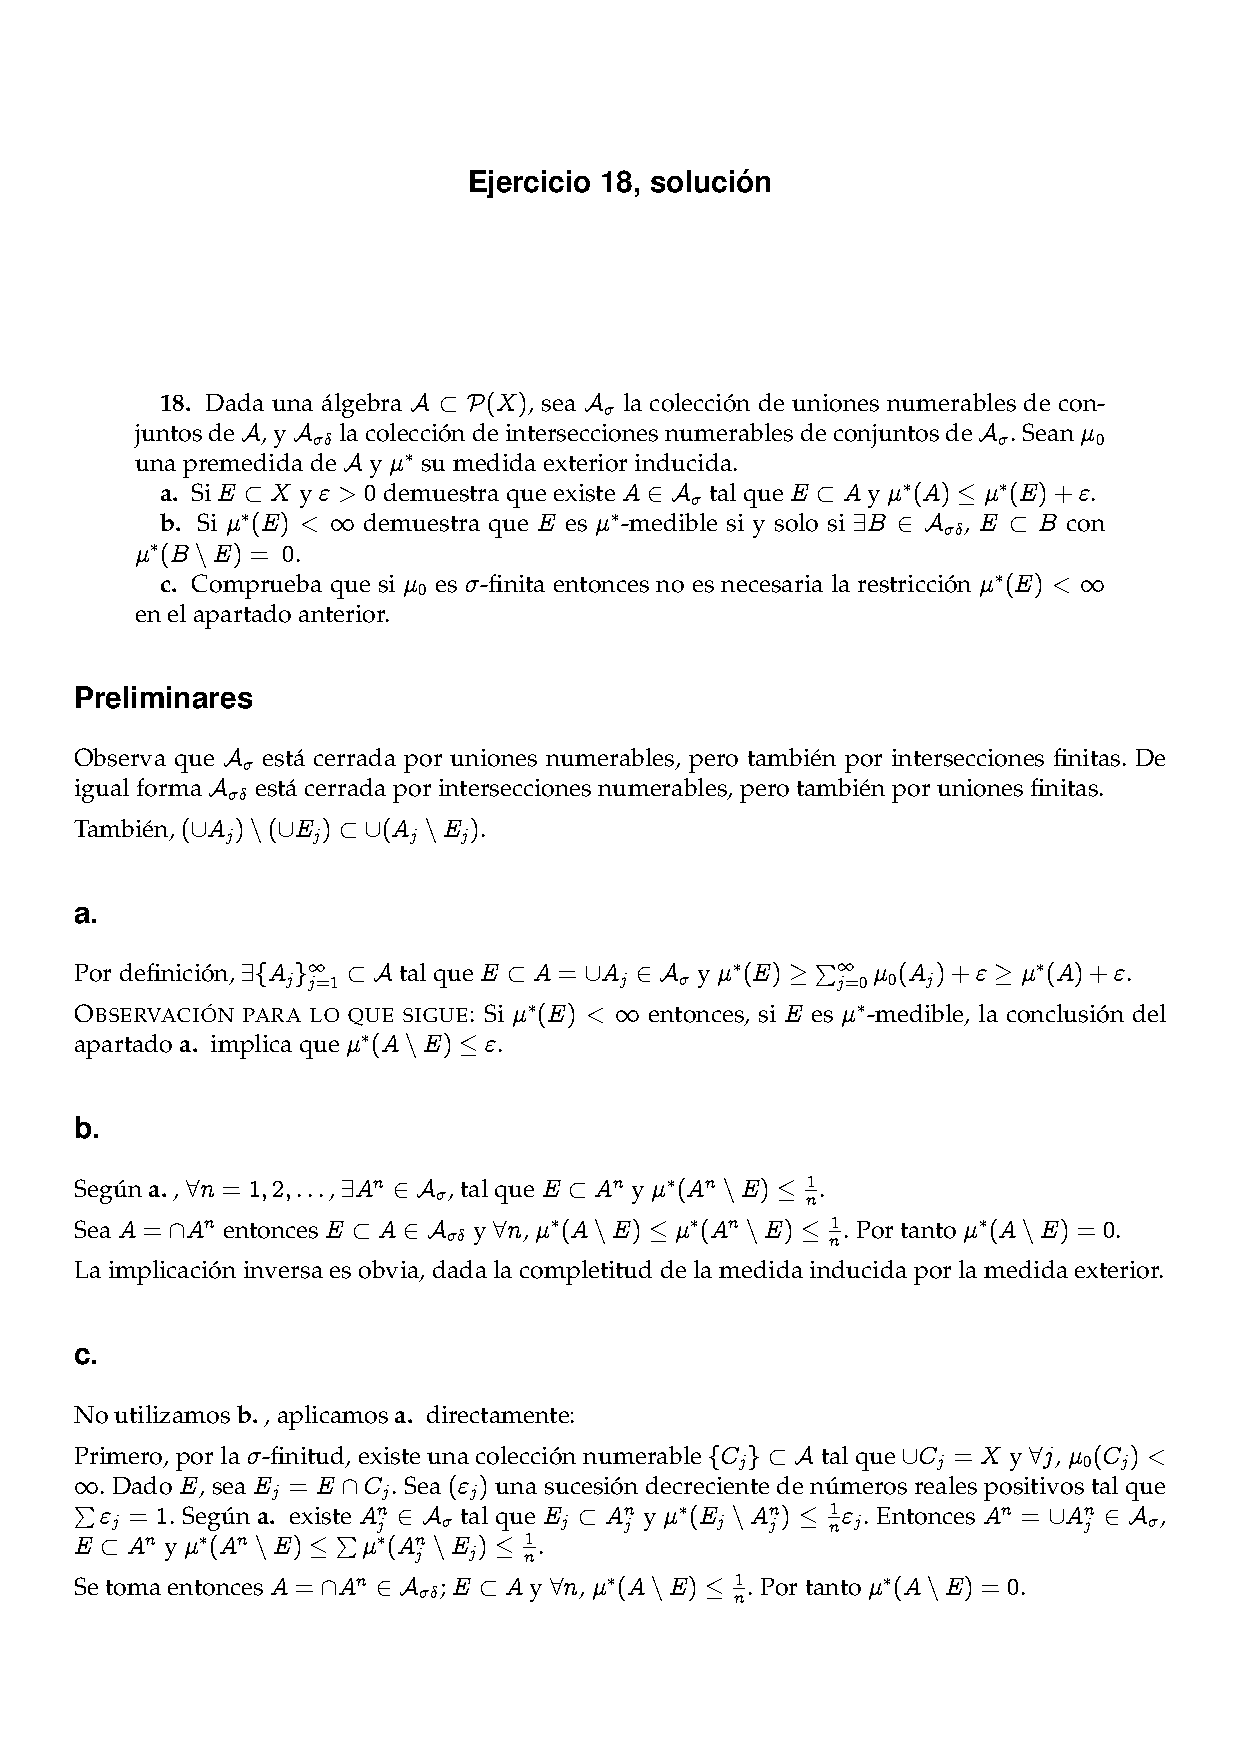
\includepdf[scale=0.9]{pdf/2014-03-18.pdf}
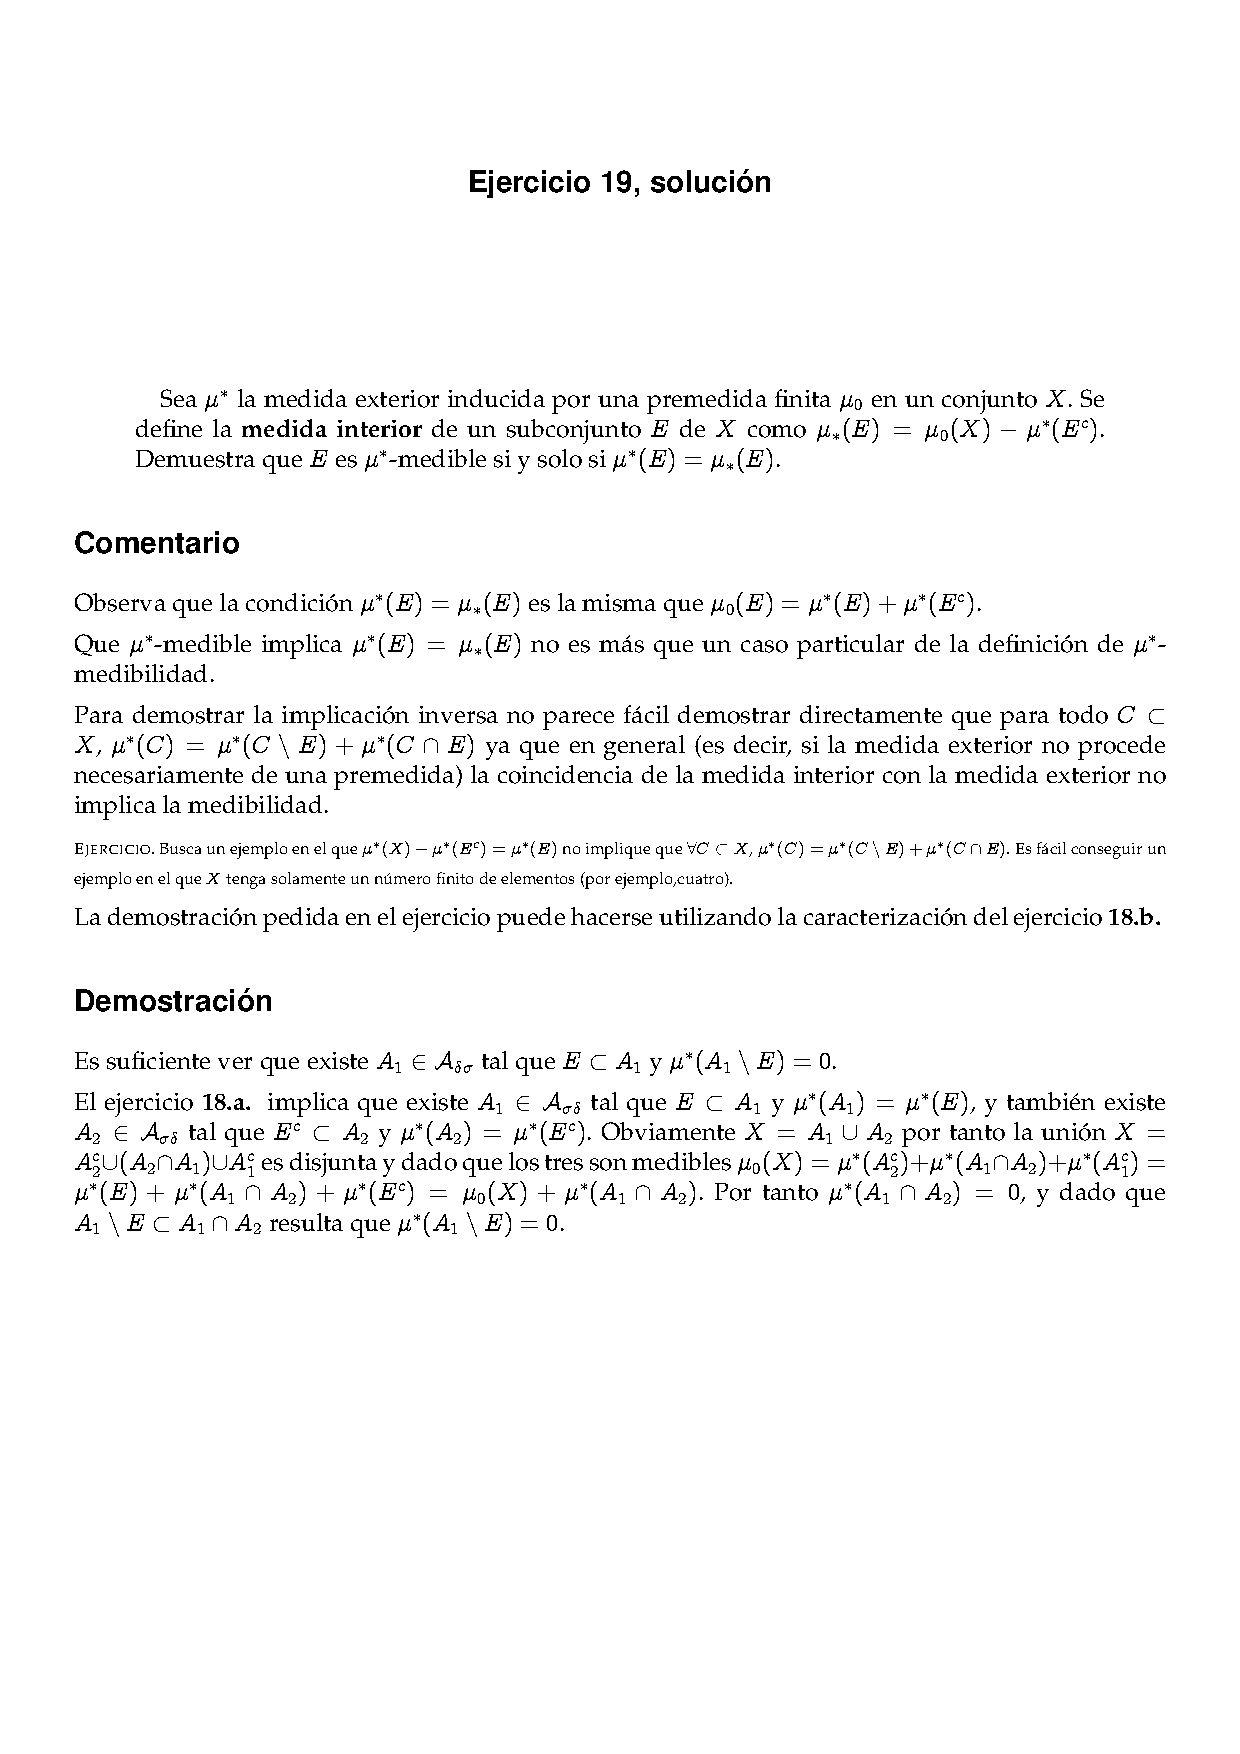
\includepdf[scale=0.9]{pdf/2014-03-19.pdf}
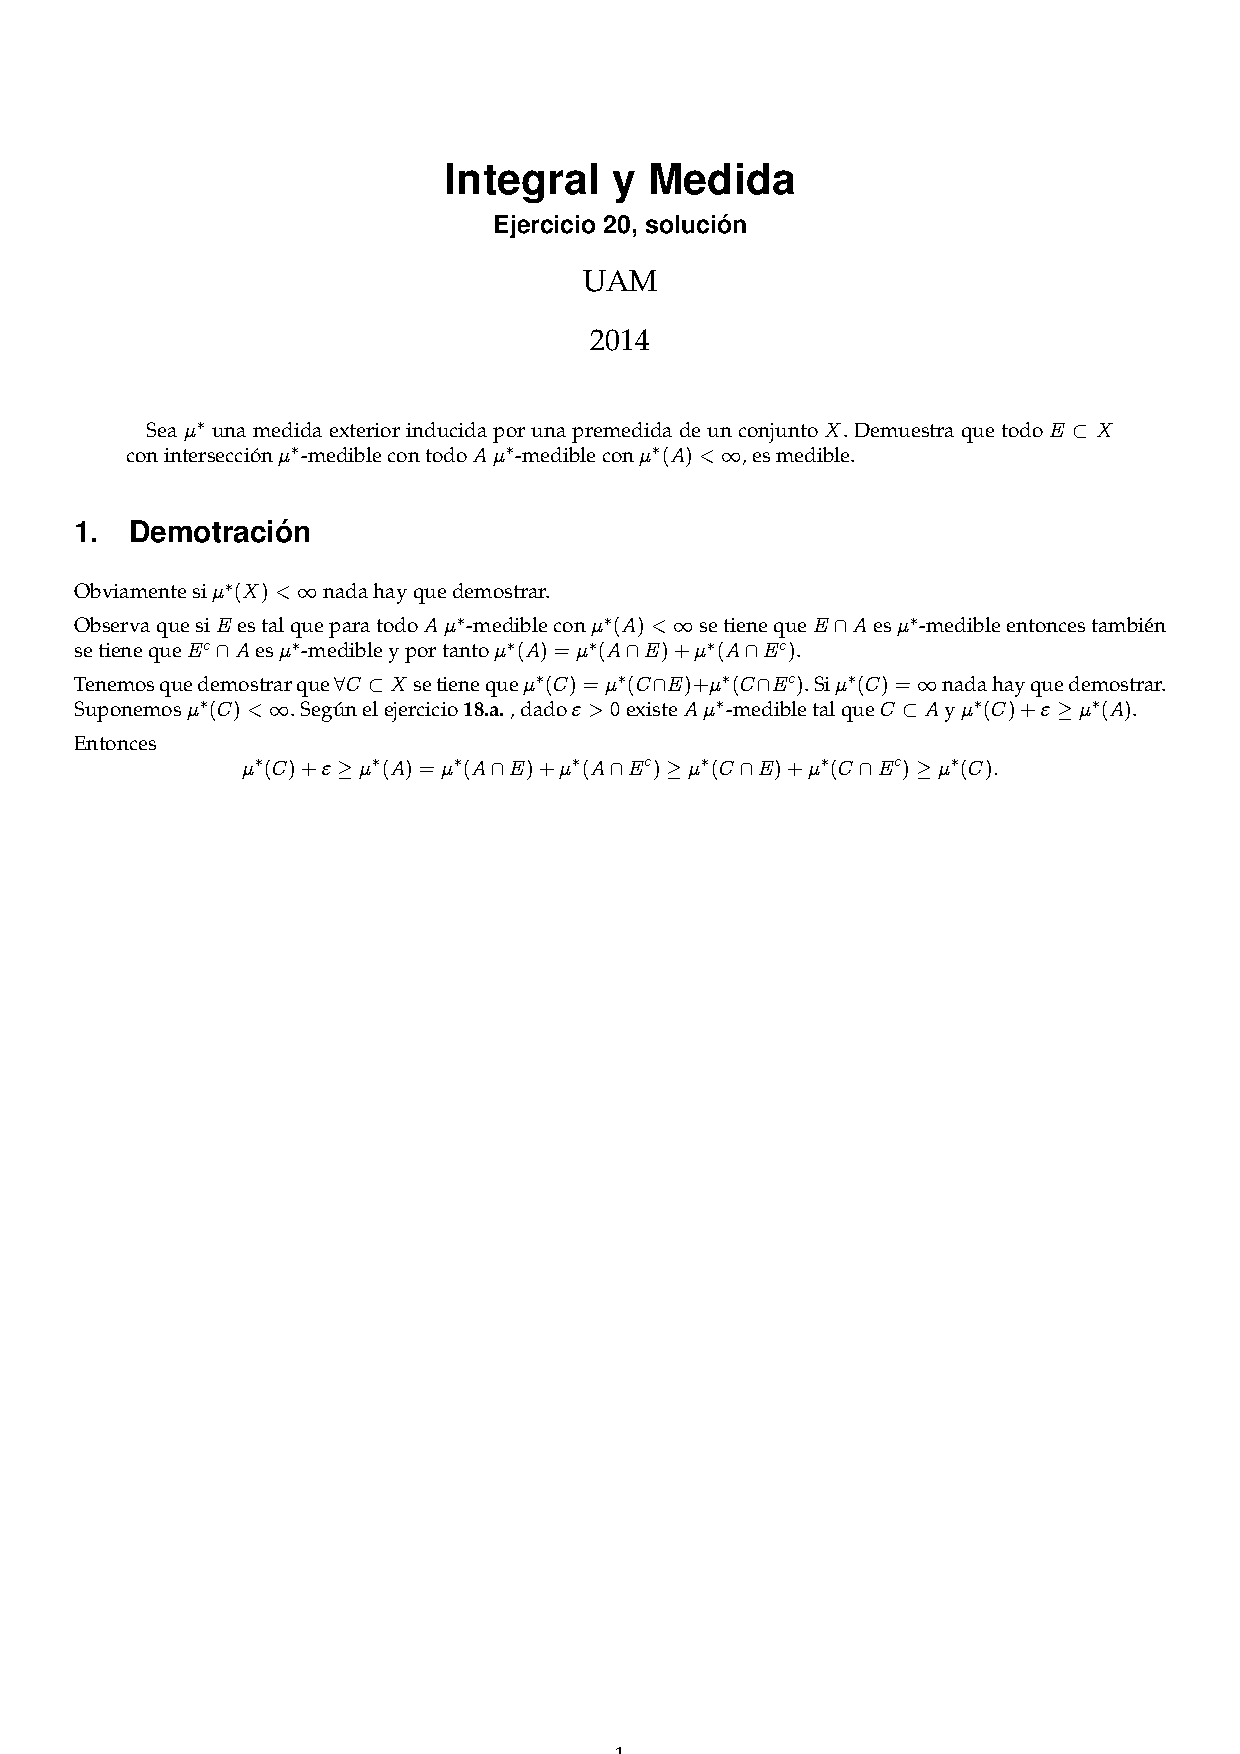
\includepdf[scale=0.9]{pdf/2014-03-20.pdf}

\subsection{Hoja 4}

\begin{problem}
Sea µ la medida de Lebesgue-Stieltjes asociada a la función:
\[F(x)=\left\{ \begin{array}{lcc}
             0 &   \text{si}  & x < 1 \\
             \\ x & \text{si} & 1 \leq x < 3 \\
             \\ 4 &  \text{si}  & 3 \leq x
             \end{array}
   \right.\]

Calcula las siguientes medidas:
\solution
\begin{itemize}
\item $µ(\{1\}) = F(1)-\displaystyle\lim_{x \to 1^-} F(x)$ = 1
\item $µ(\{2\}) = 0$
\item $µ((1, 3]) = F(3)-F(1) = 4 - 1 = 3$
\item $µ((1, 3)) = µ((1, 3]) - µ(\{3\}) = 3 - 1 = 2$
\item $µ([1, 3)) = µ((1, 3)) + µ(\{1\}) = 2 + 1 = 3$
\item $µ([1, 3])) = µ((1, 3]) + µ (\{1\}) = 3 + 1 = 4$
\end{itemize}
\end{problem}

\begin{problem}
Halla funciones de distribución $F$, $F_1$, $F_2$ de forma que, en cada caso, existan $a$ y $b$ tales que:
\begin{enumerate}
\item $µ((a,b)) < F(b)-F(a) < µ([a,b])$, donde $µ=µ_F$
\item $µ_1((a,b)) < µ_1((a,b]) < µ_1([a,b)) < µ_1([a,b])$ y

$µ_2((a,b)) < µ_2([a,b)) < µ_2((a,b]) < µ_2([a,b])$ donde $µ_i = µ_F, \ i=1,2$
\end{enumerate}
\solution
\begin{enumerate}
\item Vale con la función del ejercicio anterior
\item
\textbf{Con i = 1}
\[F_1(x)=\left\{ \begin{array}{lcc}
             0 &   si  & x < 1 \\
             \\ x & si & 1 \leq x < 3 \\
             \\ 3.5 &  si  & 3 \leq x
             \end{array}
   \right.\]

\textbf{Con i = 2}
\[F_2(x)=\left\{ \begin{array}{lcc}
             0 &   si  & x < 1 \\
             \\ x & si & 1 \leq x < 3 \\
             \\ 5 &  si  & 3 \leq x
             \end{array}
   \right.\]
\end{enumerate}

La construcción de estas funciones se ha realizado por la cuenta de la vieja. Si repetimos los cálculos del ejercicio anterior con estas funciones podemos ver que se cumplen las condiciones pedidas (Incluso puede que entendamos de qué va esto)
\end{problem}

\begin{problem}
Sea µ la medida de contar en $(\real, \algbP(\real))$. Para un conjunto finito A $\subset \real$ se define $µ_A(B) = µ(B \cap A)$ para todo $B \subset \real$

\ppart Sea $A=\{1,2,...,n,...\}$ ¿Es $µ_A$ una medida de Lebesgue-Stieltjes?. En caso afirmativo halla $F$ tal que $µ_A=µ_F$
\ppart Sea $A=\{\frac{1}{1},\frac{1}{2},...,\frac{1}{n},...\}$ ¿Es $µ_A$ una medida de Lebesgue-Stieltjes?. En caso afirmativo halla $F$ tal que $µ_A=µ_F$
\solution


\spart Esta medida simplemente cuenta el número de enteros positivos que hay en un conjunto $B$.

Por tanto, simplemente tenemos que buscar una función que realice esa misma función, por ejemplo:
\[F(x)=\left\{ \begin{array}{lcc}
             0 &   si  & 0 \leq x < 1 \\
             \\ n &  si  & n \leq x < n+1
             \end{array}
   \right.\]

Imitando las cuentas realizadas en el ejercicio 1 podemos que ver:
\begin{itemize}
\item $µ((1,3])) = F(3) - F(1) = 2$
\item $µ((1,3)) = µ((1,3])) - µ(\{3\}) = 2 - 1 = 1$
\end{itemize}
observamos que, efectivamente, obtenemos el número de enteros de cada intervalo.

\spart Esta medida cuenta el número de racionales de la forma $\frac{1}{n}$ que hay en un conjunto.

Esta medida no es de Lebesgue-Stieltjes. Una medida de Lebesgue-Stieltjes tiene que tener asociada una función $F$ como en el apartado anterior, es decir, tal que $μ((a,b]) = F(b) - F(a)$, y esta no puede tenerla.

Veamos por qué: tomemos el intervalo $B = (0,ε)$. Su medida según $μ_A$ es infinita, ya que para todo $n$ mayor que $\frac{1}{ε}$, $\frac{1}{n} ∈ A$, y entonces $B∩A$ es infinito. Luego tenemos que encontrar un $F$ tal que $F(ε) - F(0) = ∞$, y la única forma de que eso tenga sentido es que $F(ε) = ∞\; ∀ε$, lo cual es absurdo.

\end{problem}

\begin{problem}
Sea $F$ la función de distribución
\[F(x)=\left\{ \begin{array}{lcc}
             0 &   si  & x \in (-\infty, -1) \\
             \\ 1+x & si & x \in [-1, 0) \\
             \\ 2+x^2 & si & x \in [0, 2) \\
             \\ 9 &  si  & x \in [2, \infty)
             \end{array}
   \right.\]

Siendo $µ=µ_F$, hallar las siguientes medidas.
\solution
\begin{itemize}
\item $µ(\{2\}) = 3 $
\item $µ([-\frac{1}{2}, 3)) = 9 - \frac{1}{2}$
\item $µ((-1,0]\cup (1,2)) = 1 + µ((1,2]) - µ(\{2\}) = 1 + 9 -3 - 3 = 4$
\item $µ([0, \frac{1}{2}) \cup (1, 2]) = \frac{1}{4} + 6$
\item $µ(\{x \in \real \tq |x|+2x^2 > 1\})$=$µ((-\infty, -\frac{1}{2})) + µ((\frac{1}{2}, \infty)) = 0 + 9 - 2 - \frac{1}{4} = 7 - \frac{1}{4}$
\end{itemize}
\end{problem}

\begin{problem}
Sea $\appl{f}{\real}{\real}$ no negativa, integrable Riemann sobre cada intervalo finito y tal que $\int_{-\infty}^{\infty}f(x)=1$.

Prueba que $F(x)=\int_{-\infty}^x f(y) \dif y$ es una función de distribución de probabilidad y que, además, $F$ es continua ($f$ es la función de densidad de $F$).

Si $f(x)=\ind_{[0,1]}$ hallar $F$

\solution
Simplemente tenemos que ver que $F$ es no decreciente, continua por la derecha y que se cumple:
\[\lim_{n \to - \infty}F(x)=0 \ \ \lim_{n \to \infty}F(x)=1\]

Observando que $F$ es una integral y que integrar una función equivale a calcular el área encerrada bajo ella, vemos que a medida que avanzamos la $x$, cada vez estamos calculando un área mayor, luego los dos límites anteriores se cumplen.

Para ver que es continua por la derecha observamos que:
\[ \lim_{h \to 0^+}F(x+h) = \lim_{h \to 0^+} \int_{-\infty}^{x+h}f(y)\dif y = \int_{-\infty}^xf(y)\dif y = F(x)\]

Y es que por ser $F$ una integral, es obvio que es continua.

Suponemos ahora $f(x)=\ind_{[0,1]}$, para responder a la segunda pregunta del enunciado. Entonces
\[F(x)= \int_{-\infty}^{x} \ind_{[0,1]} = \left\{ \begin{array}{lcc}
             0 &   si  & x < 0 \\
             \\ x & si &  0 \leq x \leq 1 \\
             \\ 1 &  si  & 1 \leq x
             \end{array}
   \right.\]
\end{problem}

\begin{problem}
Halla el valor de $k$ para que $f= kx(1-x)\ind_{[0, 1)}$ sea la función de densidad de una medida de probabilidad. Calcula su función de distribución.

\solution
Para que sea función de densidad necesitamos que:
\[\int_{-\infty}^{\infty}f(x) dx = 1\]

Vamos a ver cuánto vale esa integral.
\begin{gather*}
\int_{-\infty}^{\infty}f(x) \dif x = \int_{-\infty}^{\infty}kx(1-x)\ind_{[0, 1)} \dif x  = \\
 = \int_{-\infty}^{0} kx(1-x)\cdot 0 \dif x + \int_{0}^{1}kx(1-x)\dif x + \int_{1}^{\infty}kx(1-x)\cdot 0 \dif x = \\
= k\left(\frac{1}{2}-\frac{1}{3}\right)
\end{gather*}


De donde obtenemos fácilmente que $k = \frac{1}{\frac{1}{2}-\frac{1}{3}} = 6$

La función de distribución sería:
\[\F(x)= \int_{-\infty}^{x} \ind_{[0,1]} = \left\{ \begin{array}{lcc}
             0 &   si  & x < 0 \\
             \\ \int_{0}^{x}kt(1-t)\dif t = (3x^2-2)x^3)& si &  0 \leq x \leq 1 \\
             \\ 1 &  si  & 1 \leq x
             \end{array}
   \right.\]
\end{problem}

\newpage
\begin{problem}
Dado $k$ > 0, sea $f(x)=αe^{-kx}\ind_{[0, \infty)}(x)$
\begin{enumerate}
\item Halla α para que $f$ sea una función de densidad de probabilidad
\item Sea $X$ una variable aleatoria con función de densidad f, si $k=\frac{1}{2}$, calcula la probabilidad de que $X \geq 3$
\item Si $k=\frac{1}{2}$ calcula la probabilidad de que $3 \leq X \leq 6$
\end{enumerate}
\solution
\begin{enumerate}
\item Repitiendo el proceso del ejercicio anterior, debemos hacer que $\int_{0}^{\infty}f(x)dx =1$.

En este caso obtenemos que α=k, es decir, nos encontramos ante una exponencial.

\item
\[\mathbb{P}(X \geq 3) = \int_{³}^{\infty}e^{-kx}dx=e^{\frac{3}{2}}\]

\item Puesto que la función de distribución es continua, la probabilidad de que $X=3$ ó $X=6$ es 0, de modo que podemos calcular la probabilidad pedida como:
\[\mathbb{P}(3 \leq X \leq 6) = \int_{3}^{6}e^{-kx}dx\]
\end{enumerate}
\end{problem}

\begin{problem}
Sea µ la medida de probabilidad definida por la función de distribución:

\[F(x)= \int_{-\infty}^{x} \ind_{[0,1]} = \left\{ \begin{array}{lcc}
             0 &   si  & x \in (- \infty, -1) \\
             \\ \frac{1}{3} & si &  x \in [-1, \sqrt{2}) \\
             \\ \frac{1}{2} + \frac{x-\sqrt{2}}{10} & si &  x \in [\sqrt{2}, 5) \\
             \\ 1 &  si  & x \in [5, \infty)
             \end{array}
   \right.\]

Calcular las siguientes medidas:
\solution

Antes de nada deberíamos comprobar que la función $F(x)$ dada es, efectivamente, una función de distribución. Para ello debemos comprobar que siempre es positiva y que se trata de una función creciente.

En este caso nos fiamos y se deja como ejercicio para el lector desconfiado (Edu) la comprobación de estas propiedades.
\newpage
\begin{enumerate}
\item \[µ((\real \setminus \rac)\cap[\sqrt{2}, 5]) = µ([\sqrt{2}, 5)) = µ((\sqrt{2}, 5]) + µ (\{\sqrt{2}\}) - µ (\{\sqrt{5}\}) =\]
\[ = F(5) - F(\sqrt{2}) +(\frac{1}{2}-\frac{1}{3}) -(1-(1-\frac{\sqrt{2}}{10}))=1-\frac{1}{2}+\frac{1}{6}-\frac{\sqrt{2}}{10}\]

\item \[µ((\real \setminus \rac)\cap [-2, \sqrt{2}]) = µ(\{\sqrt{2}\}) = \frac{1}{2}-\frac{1}{3} = \frac{1}{6}\]

\item \[µ(\rac \cap [1,6]) = µ(\{5\}) = \frac{\sqrt{2}}{10}\]
\end{enumerate}

Vamos ahora a por la parte complicada del ejercicio.

\[A_{3n-2} = \left(\frac{2n}{4n+3}, \frac{4n+5}{3n}\right)\]
\[A_{3n} = \left(\frac{4}{5n+2}, \frac{6n+1}{2n}\right)\]
\[A_{3n-1} = \left(-2, \frac{6n-1}{5n+2}\right)\]

Vemos que:
\begin{enumerate}
	\item $\lim A_{3n-2}= [\frac{1}{2}, \frac{4}{3}]$
	\item $\lim A_n{3n-1} = (-2, \frac{6}{5})$
	\item $\lim A_{3n} = (0^+, 3^+)$
\end{enumerate}

Recordemos que el límite superior de $A_n$ es el conjunto de puntos que están en infinitos conjuntos de la sucesión. Por tanto, todos los puntos contenidos en estos límites se contienen en el límite superior de la sucesión.
\[\limsup A_n = [\frac{1}{2}, \frac{4}{3}] \bigcup  (-2, \frac{6}{5}) \bigcup (0^+, 3^+)\]

Por otro lado, el límite inferior es el conjunto de puntos que se encuentran en todos los elementos de la sucesión a partir de uno dado. Así, el límite inferior será la intersección de los límites calculados anteriormente.
\[\liminf A_n = [\frac{1}{2}, \frac{4}{3}] \bigcap  (-2, \frac{6}{5}) \bigcap (0^+, 3^+)\]

\textcolor{blue}{Completado por mi. No fiarse al 100\%}
\[µ(\limsup A_n) = µ([\frac{1}{2}, \frac{4}{3}]) +  µ((-2, \frac{6}{5})) +µ((0^+, 3^+)) = \frac{1}{3}  + \frac{1}{3} + \frac{1}{3} = 1\]
\[µ(\liminf A_n) = µ([\frac{1}{2}, \frac{6}{5})) = 0\]

\end{problem}

\begin{problem}
Sea $\appl{F}{\real}{\real}$ una función de distribución
\begin{enumerate}
\item Prueba que el conjunto de puntos de discontinuidad de $F$ es numerable
\item Prueba que el conjunto de puntos de continuidad de $F$ es denso en $\real$
\end{enumerate}
\obs $F$ es monótona luego no tiene más discontinuidades que saltos
\solution

\begin{enumerate}
\item Vamos a probar que el número de puntos de discontinuidad en (n, n+1] es numerable.

Para ello tomamos la medida de este intervalo:
\[M = F(n+1)-F(n)\]

La pregunta que nos hacemos ahora es, ¿cuántos puntos $x \in (n, n+1]$ pueden tener $µ_F(\{x\}) \frac{M}{k}$?

La respuesta es sencilla (la supo hasta Elena en clase). $\forall k \in \nat$ No podemos tener más de k puntos con esta condición.

Por tanto no puede haber una cantidad no numerable de puntos de (n, n+1] con $µ_F(\{x\})>0$
%\item Si tuviésemos una cantidad no numerable de discontinuidades tendríamos un intervalo cerrado que contiene una cantidad no numerable de discontinuidades. Puesto que cada una de esas discontinuidades tenemos un salto, resulta que tendríamos un número no numerable de saltos en un intervalo cerrado.

%Así, tendríamos que la medida del intervalo cerrado sería la suma infinita y no numerable de valores positivos, lo que nos daría un resultado finito.

%Leyendo de un artículo de wikipedia:
%\begin{verbatim}
%La suma de los saltos no puede ser mayor que la diferencia de los
%valores de la función en los extremos del intervalo, de modo que
%el conjunto de discontinuidades con salto mayor que 1/n es finito
%y, por tanto, el conjunto de discontinuidades es a lo más numerable
%\end{verbatim}

\item \textcolor{blue}{Hecho por mi. No fiarse al 100\%}

Recordando lo dado en topología, sabemos que un conjunto es denso si la adherencia del conjunto coincide con el total.

Recordamos también que la adeherencia son aquellos puntos tales que todo abierto que lo contenta corta al conjunto dado.

Puesto que las únicas discontinuidades que puede presentar una función de distribución son discontinuidades de salto y es obvio que para cualquier punto en que la función sea continua todo entorno del punto contiene otros puntos de discontinuidad.
\end{enumerate}
\end{problem}

\begin{problem}
Variando si es necesario en cada caso el tamaño de los intervalos, construir un conjunto de tipo Cantor cuya medida de Lebesgue sea mayor que 1-ε
\solution
La construcción del conjunto de Cantor consiste en tomar el intervalo [0,1] y los siguientes conjuntos:
\begin{enumerate}
\item Construimos un intervalo $A_1$ de longitud $\frac{ε}{2}$ centrado en el intervalo [0,1].
\item Construimos $A_2 = \bigcup (a_i, b_i)$ tales que cada elemento de la unión tiene longitud igual a $\frac{1}{2}\frac{ε}{4}$.
\item etc
\end{enumerate}
Así, en el paso n-ésimo tenemos:
\[A_n = (a_1^n,b_1^n) \cup (a_2^n,b_2^n) \cup ... \cup (a_n^n,b_n^n)\]
donde cada intervalo de la unión tiene longitud $\frac{1}{2^{n-1}}\frac{ε}{2}$.

El conjunto de Cantor se obtiene restando del intervalo incial todos los intervalos $A_n$ que hemos ido construyendo. Es decir:
\[C = I -\bigcup A_n\]
\[m(C)=m(I)-\sum m(A_n) = 1 - ε\]
\end{problem}

\begin{problem}
Sea $µ_F$ la medida de Lebesgue-Stieltjes correspondiente a una función creciente y continua $\appl{F}{\real}{\real}$
\begin{enumerate}
\item Prueba que si A es numerable entonces $µ_F(A)$=0
\item Prueba que existen conjuntos A tales que $µ_F(A)> 0$ y A no contiene ningún intervalo abierto.
\item Si $µ(A)\geq 0$ y $µ(\real \setminus A) = 0$, ¿tiene que ser A denso en $\real$
\end{enumerate}
\obs Se recomienda construir una función $F(x)$ que sea constante en un intervalo
\solution

\begin{enumerate}
\item \textcolor{blue}{Hecho por mi. No fiarse al 100\%}

Si $A$ es numerable podemos escribirlo de la forma:
\[A = \bigcup_{i=1}^{\infty}\{a_i\} \tq a_i \neq a_j \forall i, j \ i \neq j\]
por tanto,
\[µ(A) = \sum_{i=1}^{\infty} µ(\{a_i\}) \]
pero, puesto que la función del enunciado es continua, la medida de un único punto siempre es 0 y por lo que
\[µ(A) = \sum_{i=1}^{\infty} µ(\{a_i\}) = \sum_{i=1}^{\infty}  0 = 0\]

\item Podemos tomar el conjunto $(a, b]$ que tendrá
\[µ((a,b]) = F(b)-F(a) \geq 0\]
ya que $F$ es creciente.

Ahora debemos cuida que no contenta abiertos. Para ello basta con tomar la intersección de este intervalo con los racionales.

Con ello eliminamos la posibilidad de que haya abiertos contenidos en el conjunto y mantenemos la medida del conjunto puesto que la medida de los racionales (que son los que estamos extrayendo) es 0.

\item No tiene por qué ser A denso. Pongamos un contraejemplo para probarlo.

Si tomo una función que crece entre el 0 y el 1 y luego se queda constante y tomo $A=(0,1)$ tenemos que se cumplen las condiciones del enunciado pero obviamente el intervalo $(0,1)$ en $\real$ no es denso.
\end{enumerate}
\end{problem}

\begin{problem}
Sea $F(x)=log(1 + |x|)\cdot \ind_{[0, \infty)}(x)$
\begin{enumerate}
\item Comprueba que $\appl{F}{\real}{\real}$ es creciente y continua por la derecha.
\item Calcula $µ_F(\{Cantor\})$
\end{enumerate}
\obs El conjunto de Cantor está contenido en $2^n$ intervalos de longitud $\frac{1}{3^n}$
\solution

\begin{enumerate}
\item \textcolor{blue}{Hecho por mi. No fiarse al 100\%}

Tenemos que ver que $a<b \implies F(a) < F(b)$ lo cual es obvio ya que el logaritmo es creciente y la función indicatriz simplemente vale 0 cuando $x4 < 0$ y 1 en el resto de casos.

Para ver que es contínua por la derecha necesitamos probar que:
\[\lim_{x \to a^+}F(x) = F(a) \ \forall a \in X\]
El único punto donde podemos dudar es en $a=0$ pero en ese caso está claro que:
\[\lim_{x \to 0^+}F(x) = \log(1) = 0 = F(0)\]

\item
\begin{defn}[Conjunto de Cantor]
Es el conjunto de todos los puntos del intervalo real [0,1] que admiten una expresión en base 3 que no utilice el dígito 1
\end{defn}

\[µ_F(\{Cantor\}) = 1 - \frac{1}{3}+2\frac{1}{9}+4\frac{1}{27}+... = \frac{1}{3} \sum_{n=1}^{\infty}\left(\frac{2}{3}\right)^{n-1} = \frac{1}{3} \frac{1}{1-\frac{2}{3}} = 1-1 = 0\]

\end{enumerate}
\end{problem}

\begin{problem}
Sea µ una medida de Borel en $\real$, finita sobre compactos, con $µ((0, 1])=1$
\begin{enumerate}
\item Prueba que si $\forall s \in \real, µ(s + E)=µ(E)$, entonces µ es la medida de Lebesgue.
\item Prueba que si $\forall s \in \real, µ(rE)=|r|µ(E)$, entonces µ es la medida de Lebesgue
\end{enumerate}
\solution
\begin{enumerate}
\item
Para ver que es la medida de Lebesgue necesitamos ver que
\[\forall a,b \ a<b \ µ((a,b]) = b-a\]
Por continuidad podemos restringirnos a trabajar con a,b racionales.

Por la invarianza por traslaciones es suficiente ver:
\[\forall b \in \rac \ µ((0,b])=b\]

Vamos a ello pues
\[µ((0, \frac{p}{q}]) = \sum_{i=1}^{\infty} µ((\frac{1-i}{q}, \frac{i}{q}]) = p\cdot µ((0, \frac{1}{q}])\]

Ahora sólo nos queda ver que $µ((0, \frac{1}{q}]) = \frac{1}{q}$, pero para ello basta con fijarnos en que:
\[µ((0, 1]) = \sum_{i=1}^{\infty} µ((\frac{i-1}{q}, \frac{i}{q}]) = q \cdot µ((0, \frac{1}{q}])\]

\item Se hace prácticamente igual que el apartado anterior. Se deja como ejercicio para casa.


\end{enumerate}
\end{problem}

\begin{problem}
Sea µ la medida de Lebesgue de $\real$ y $E \subset \real$ medible Lebesgue tal que 0 < µ(E) < $\infty$. Demuestra que para todo α, 0<α<1, existe un intervalo abierto I tal que µ($I \cap E$) > α m(I)
\solution
Sabemos que la medida de Lebesgue se puede aproximar bien por abiertos que contengan al conjunto $E$, es decir:
\[\forall ε > 0 \ \exists A \text{ abierto con } E \subset A \tq µ(E) > µ(A)-ε \]

Tomamos $A= \bigcup_{k=1}^{\infty} I_k$ con los $I_k$ disjuntos.

Suponemos ahora que $\exists α \in (0,1) \tq \forall I \text{ intervalo abierto } µ(E \cap I)\leq αµ(I)$
Entonces
\[µ(E) = \sum_{k=1}^{\infty}µ(E \cap I_k) \leq \sum_{k=1}^{\infty} α µ(I_k) = α µ(A)\]

Si la suposición fuese cierta tendríamos ahora
\[µ(A)-µ(E) \geq µ(A) - α µ(A) (1-α)µ(A) \geq (1-α)µ(E) > ε\]
y llegamos a contradicción.
\end{problem}



\printindex
\end{document}

